\documentclass[final,fmstyle]{./util/ucathesis}
% La opcion 'final' muestra los graficos, para generar una version sin los graficos utiliza la opcion 'draft'

% paquetes recomendados
%\usepackage[chapter]{theorems}
%\usepackage{symbols}
%\usepackage{url}
\usepackage{amsmath,amsthm}

\usepackage[T1]{fontenc}
\usepackage[spanish]{babel}
\usepackage[utf8]{inputenc}
\usepackage{csquotes}
\usepackage[style=numeric,sorting=none,backend=biber]{biblatex}
\usepackage{tabularx}
\usepackage{pdflscape}
\usepackage{listings}
\usepackage{subfigure}
\addbibresource{referencias.bib}


% custom commands
\newcommand{\foreign}[1]{{\it #1}}
\DeclareMathOperator*{\argmax}{arg\,max}
\algsetup{indent=2em}

% \setcounter{tocdepth}{3}

% datos de la tesis
\title{Dise\~{n}o de Interfaces de Usuario basado en Reconocimiento del Habla}
\author{Rodrigo Manuel Parra Zacar\'{i}as y Jorge Daniel Ram\'{i}rez Medina}
\degree{Inform\'{a}tica}

\advisor{Ing.}{Mart\'{i}n Abente Lahaye,M.Sc.}

%\newtheorem{definicion}{Definicin}
%\numberwithin{algorithm}{chapter}

\logosource{./graphics/logo.jpg}
\institution{Universidad Nacional de Asunci\'{o}n}
\faculty{Facultad Polit\'{e}cnica}
\address{San Lorenzo - Paraguay}

\begin{document}

\maketitle     % esto hace las portadas

% Agradecimientos
%%!TEX root = ../tesis.tex
\chapter*{Agradecimientos}

A \textbf{Martín Abente Lahaye}, por la orientación y el acompañamiento constantes 
proporcionados durante el desarrollo de este trabajo.

A la \textbf{Facultad Politécnica de la UNA}, por los años de formación académica recibidos, los cuales 
nos enorgullecen y nos comprometen a representar siempre de la mejor manera a tan distinguida casa de 
estudios.

A los \textbf{profesores y alumnos} de nuestra carrera que colaboraron con la realización 
de este trabajo mediante el presente más valioso que puede entregarse: el tiempo. 

A nuestros \textbf{amigos}, los que hicimos durante los años de carrera universitaria y los que vienen
de antes, cuyo apoyo incondicional hizo más pequeños los obstáculos y más cercana la meta.

A nuestras \textbf{familias}, que inspiran, acompañan y dan sentido a cada uno de nuestros pasos. La vida probablemente no alcance para devolver todo lo que hemos recibido de ellas. Este logro es tan suyo como nuestro.

A \textbf{Dios}, sin cuya bendición nada de esto hubiese sido posible.


% los siguientes comandos producen 'indices.

% Tabla de contenidos
\tableofcontents
% Lista de figuras
\listoffigures
% Lista de tablas
\listoftables
% Lista de algoritmos
\listofalgorithms
%\newacronym{rca}{RCA}{\foreign{Radio Corporation of America}}
\newacronym{mit}{MIT}{Instituto Tecnol\'ogico de Massachusetts}
\newacronym{nec}{NEC}{\foreign{Nippon Electric Company}}
\newacronym{hmm}{HMM}{modelo oculto de Markov}
\newacronym{ibm}{IBM}{\foreign{International Business Machines}}
\newacronym{arpa}{ARPA}{Agencia de Proyectos de Investigaci\'on Avanzada}
\newacronym{cmu}{CMU}{Universidad Carnegie Mellon}
\newacronym{hwim}{HWIM}{\foreign{Hear What I Mean}}
\newacronym{bbn}{BBN}{\foreign{Bolt, Beranek and Newman Technologies}}
\newacronym{pdp}{PDP}{procesamiento distribuido en paralelo}
\newacronym{att}{AT\&T}{\foreign{American Telephone and Telegraph}}
\newacronym{darpa}{DARPA}{Agencia de Proyectos de Investigaci\'on Avanzados de Defensa}
\newacronym{ears}{EARS}{\foreign{Effective Affordable Reusable Speech-to-Text}}
\newacronym{csj}{CSJ}{Corpus de Japon\'es Espont\'aneo}
\newacronym{cm}{CM}{medidas de confianza}
\newacronym{api}{API}{interfaz de programaci\'on de aplicaciones}
\newacronym{wer}{WER}{tasa de error por palabra}
\newacronym{nato}{NATO}{Organizaci\'on del Tratado del Atl\'antico Norte}
\newacronym{asr}{ASR}{reconocimiento autom\'atico del habla}
\newacronym{nsr}{NSR}{Red de reconocimiento del habla}
\newacronym{dsr}{DSR}{Reconocimiento del habla distribuido}
\newacronym{wami}{WAMI}{\foreign{WAMI Toolkit}}
\newacronym{vrcp}{VRCP}{\foreign{Voice Recognition Call Processing}}
\newacronym{nortel}{NORTEL}{\foreign{Northern Telecom Limited}}
\newacronym{aabs}{AABS}{\foreign{Adaptive Antenna Beam Selection}}
\newacronym{rtf}{RTF}{factor de tiempo real}
\newacronym{fdp}{FDP}{Funci\'on de Densidad de Probabilidad}
\newacronym{lpc}{LPC}{Codificaci\'on Predictiva Lineal}
\newacronym{dtw}{DTW}{Distorsi\'on Din\'amica Temporal}
\newacronym{rna}{RNA}{Red Neuronal Artificial}
\newacronym{mlp}{MLP}{Perceptr\'on Multicapa}
\newacronym{jsgf}{JSGF}{\foreign{Java Speech Grammar Format}}
\newacronym{olpc}{OLPC}{Una Computadora por Ni\~no}
\newacronym{htk}{HTK}{\foreign{Hidden Markov Model Toolkit}}
\newacronym{bsd}{BSD}{\foreign{Berkeley Software Distribution}}
\newacronym{fst}{FST}{Transductor de estado finito}
\newacronym{sdk}{SDK}{\foreign{Software Development Kit}}
\newacronym{rest}{REST}{\foreign{Representational State Transfer}}
\newacronym{pti}{PTI}{Parque Tecnol\'ogico Itaipu}











%\include{simbolos}

\mainmatter  % inician los capitulos de la tesis

% incluye aqui los capitulos (un archivo .tex por capitulo)
%!TEX root = ../tesis.tex
\chapter{Introducci\'on}
\label{sec:intro}

El habla, y m\'as concretamente el lenguaje como medio de comunicaci\'on, es una
de las caracter{\'\i}sticas fundamentales que diferencian al ser humano de los dem\'as
animales y representa un factor clave de su evoluci\'on \cite{SchepartzLanguage1993}. La misma es considerada
el principal modo de comunicaci\'on y la forma m\'as eficiente y natural de intercambio 
de informaci\'on entre seres humanos \cite{GaikwadAReview2010}.

Atendiendo la importancia de la voz y el habla en la comunicaci\'on entre personas,
resulta l\'ogico el inter\'es por desarrollar tecnolog{\'\i}as que permiten una interacci\'on
similar entre una persona y una computadora. Es decir, resulta interesante la idea 
de ``hablar'' con una computadora.

El reconocimiento del habla, tambi\'en conocido como reconocimiento autom\'a-
tico del habla, es el proceso de convertir una se\~nal de voz en una secuencia de
palabras, mediante un algoritmo implementado program\'aticamente \cite{JaisalAReview2012}. Su inte-
graci\'on con interfaces de usuario busca una interacci\'on humano-computadora m\'as
natural, de manera a superar las limitaciones existentes en el modelo convencional
de interacci\'on.

Los asistentes virtuales de Apple \cite{AppleSiri} y Google \cite{GoogleNow}, 
los centros de mando en los autom\'oviles de Ford \cite{FordSync} y Toyota \cite{ToyotaEntune},
y los SmartTV de Samsung \cite{SamsungVoiceControl}; todos ellos capaces de reaccionar a 
comandos por voz del usuario, son ejemplos de la incorporaci\'on de interfaces basadas 
en reconocimiento del habla en actividades de la vida diaria.

Los resultados de los estudios realizados por la respetada consultora tecnol\'ogica
Gartner confirman esta tendencia. Estos ubican al reconocimiento del habla entre
las tecnolog{\'\i}as que se estabilizar\'an, y cuyos beneficios estar\'an ampliamente
demostrados, en los pr\'oximos 2 a 5 a\~nos \cite{Gartner2013}. 

El escenario descrito resulta propicio para la investigaci\'on en el \'area.
Teniendo esto en cuenta, resulta importante contar con un estudio te\'orico
y pr\'actico del reconocimiento del habla, desde sus fundamentos hasta su
aplicaci\'on. El estudio ser{\'\i}a de gran utilidad como material introductorio
para quien quisiese estudiar y aplicar el reconocimiento del habla, pudiendo
servir de base para numerosos trabajos futuros.

Este es el eje central de este trabajo final de grado, cuyos objetivos y organizaci\'on se
exponen a continuaci\'on.

\section{Objetivo General}
\label{sec:objgral}

Realizar un estudio cient\'{i}fico del trasfondo hist\'{o}rico, los fundamentos te\'{o}ricos 
y el estado del arte del reconocimiento del habla de modo a comprender y describir 
esta \'{a}rea de investigaci\'{o}n.  


\section{Objetivos Espec\'{i}ficos}
\label{sec:objspec}

\begin{itemize}
    \item Analizar, ordenar y caracterizar el proceso t\'{i}pico de un sistema de reconocimiento del habla, 
        incluyendo los aspectos te\'{o}ricos involucrados en cada paso del mismo.

    \item Evaluar y seleccionar las herramientas disponibles que permiten la implementaci\'{o}n de soluciones 
        relacionadas al reconocimiento del habla.
    
    \item Dise\~{n}ar e implementar una interfaz mediante voz del usuario de manera a aplicar y 
    contrastar en la pr\'{a}ctica los conocimientos te\'{o}ricos adquiridos.
    
    \item Evaluar la soluci\'{o}n implementada de modo a obtener resultados experimentales comparativos que 
        permitan extraer conclusiones sobre la aplicabilidad del reconocimiento del habla a las interfaces 
        de usuario.
\end{itemize}

\section{Organizaci\'on del Trabajo}
\label{sec:organizacion}


El presente trabajo est\'a organizado como se describe a continuaci\'on:

\begin{itemize}
	\item En el cap{\'\i}tulo 2 se presenta un breve resumen de los antecedentes hist\'oricos del reconocimiento
	del habla, desde sus inicios hasta la actualidad.
	\item En el cap{\'\i}tulo 3 se presentan varias \'areas de aplicaci\'on del reconocimiento del habla, 
	mencionando avances y algunos trabajos de referencia en cada una.
	\item En el cap{\'\i}tulo 4 se presenta el proceso t\'{i}pico de un sistema de reconocimiento del habla,
	describiendo algunos fundamentos matem\'aticos y algoritmos relacionados a cada paso.
	\item En el cap{\'\i}tulo 5 se presentan algunas medidas de desempe\~no de sistemas de reconocimiento del
	habla, incluy\'endose resultados obtenidos en trabajos de investigaci\'on con respecto a cada una.
	\item En el cap{\'\i}tulo 6 se presentan los resultados de un estudio comparativo de las tecnolog{\'\i}as
	y herramientas disponibles para la implementaci\'on de sistemas de reconocimiento del habla.
	\item En el cap{\'\i}tulo 7 se presenta el problema planteado a modo de llevar a la pr\'actica los
	conocimiento te\'oricos aprendidos.
	\item En el cap{\'\i}tulo 8 se presenta la soluci\'on propuesta para el problema planteado, incluyendo
	las herramientas a utilizar y otros detalles de implementaci\'on.
	\item En el cap{\'\i}tulo 9 se presentan los aspectos relacionados a la evaluaci\'on realizada una vez
	implementada la soluci\'on. Se mencionan los objectivos y se describen la metodolog{\'\i}a utilizada
	y las variables que se tuvieron en cuenta.
	\item En el cap{\'\i}tulo 10 se presentan los resultados obtenidos una vez realizada la evaluaci\'on
	del trabajo.
	\item En el cap{\'\i}tulo 11 se presentan las conclusiones obtenidas a trav\'es de las distintas
	etapas de realizaci\'on del trabajo, desde las investigaciones iniciales hasta la evaluaci\'on.
	\item Finalmente, en el cap{\'\i}tulo 12 se presentan algunas oportunidades posibles para
	la realizaci\'on de trabajos futuros en el \'area.
\end{itemize}
%!TEX root = ../tesis.tex
\chapter{Historia del Reconocimiento del Habla}
\label{sec:antecedentes}

El progreso del reconocimiento del habla, desde las primeras publicaciones cient\'{i}ficas sobre
an\'{a}lisis y s\'{i}ntesis del habla en la primera mitad del siglo XX hasta llegar a las respuestas 
r\'{a}pidas y cargadas de humor de asistentes virtuales inteligentes como Siri, es el producto de d\'{e}cadas 
de investigaci\'{o}n motivadas por el sue\~{n}o de construir una m\'{a}quina capaz de mantener una 
conversaci\'{o}n con un ser humano.

Este cap\'{i}tulo presenta una s\'{i}ntesis de acontecimientos significativos relacionados al
desarrollo del reconocimiento del habla desde sus inicios. Aunque resulte dif\'{i}cil abarcar casi un siglo
de avances en pocas p\'{a}ginas, este repaso hist\'{o}rico puede resultar de utilidad para comprender el
panorama actual y la perspectiva a futuro de esta importante \'{a}rea de investigaci\'{o}n.

\section{Antes de 1950}
\label{sec:pre50s}

Los primeros intentos por parte de la comunidad cient\'{i}fica de construir sistemas de 
reconocimiento autom\'{a}tico del habla no se dieron hasta la d\'{e}cada de los 50. 
Sin embargo, la primera m\'{a}quina capaz de respondera un comando de voz fue Radio Rex, 
un juguete fabricado en \mbox{1920 \cite{AnusuyaSpeech2009}}.

Radio Rex era un peque\~{n}o perro de pl\'{a}stico sobre una base de hierro que se manten\'{i}a dentro de una casita
mediante la fuerza de atracci\'{o}n de un im\'{a}n alimentado por un conductor sensible a una frecuencia de 500 Hz.
La presencia de una onda a esta frecuencia causaba vibraci\'{o}n en el conductor, interrumpiendo de
esta manera la corriente y causando que Rex saliese de su casa. 

El sonido de la ``e'' en Rex posee una componente correspondiente a 500 Hz, lo cual le permit\'{i}a al can responder a su nombre.

En el \'{a}mbito acad\'{e}mico, cabe destacar la investigaci\'{o}n conducida por Fletcher en los laboratorios Bell
durante los a\~{n}os 20 sobre la relaci'{o}n entre el espectro de una se\~{n}al de voz (distribuci\'{o}n de 
la amplitud a trav\'{e}s de la frecuencia) sobre el sonido percibido por un ser humano \cite{FletcherNature1922}. 
Las conclusiones de este trabajo ser\'{i}an de gran influencia para el desarrollo del sintetizador de habla VODER por parte de Dudley en la siguiente \mbox{d\'{e}cada \cite{JuangAutomaticSpeech}}. 

\section{1950 - 1960}
\label{sec:50s}

Los inicios del reconocimiento del habla fueron bastante limitados. Esto se debi\'o a que el procesamiento 
de se\~{n}ales y tecnolog\'{i}as computacionales eran a\'un bastante primitivas. 

La mayor\'{i}a de los sistemas desarrollados utilizaron las resonancias espectrales de las vocales,
extra{\'\i}das a partir de las se\~nales de salida de un banco de filtros anal\'{o}gicos y 
circuitos l\'ogicos \cite{Furui50Years2004}.
 
En esta \'{e}poca varios investigadores intentaron explotar las ideas fundamentales propuestas por 
la fon\'{e}tica ac\'{u}stica \cite{AnusuyaSpeech2009}, que describe el habla en t\'{e}rminos de 
elementos fon\'{e}ticos (los sonidos b\'{a}sicos de un lenguaje) y trata de
explicar c\'{o}mo son generados ac\'{u}sticamente al hablar \cite{JuangAutomaticSpeech}. 
Este conjunto de elementos incluye a los fonemas, la posici\'on y los modos de articulaci\'on 
de los \'organos del aparato fonador, como la boca y las cuerdas vocales, utilizados para 
producir los sonidos en varios contextos fon\'{e}ticos.

Los formantes son muy importantes en el proceso humano de reconocimiento del habla, estos son 
bandas de frecuencias en donde se concentra gran parte de la energ\'{i}a en el espectro de un 
sonido \cite{HawkinsAcoustic2009}. Los estudios de la estructura de los formantes sirvieron 
como gu\'{i}a para que investigadores de los Laboratorios Bell crearan, en 1952, un reconocedor
autom\'{a}tico de d\'{i}gitos, denominado \foreign{Audrey} \cite{DavisAutomatic1952}.

Teniendo en cuenta la naturaleza estad\'{i}stica del habla, Audrey utilizaba un proceso de 
correspondencia de patrones para identificar los d\'{i}gitos. Esta correspondencia de patrones 
involucraba comparar caracter\'{i}sticas derivadas de una se\~{n}al desconocida con otras 
caracter\'{i}sticas derivadas de una se\~{n}al conocida. La precisi\'{o}n de
Audrey variaba entre 97 y 99 por ciento, habi\'endose realizado un ajuste previo al hablante,
si los d\'{i}gitos eran pronunciados con una pausa de 350 ms\cite{DavisAutomatic1952}.

En otros sistemas de reconocimiento que datan de esta \'{e}poca, Olson y Belar de los Laboratorios 
de la \gls{rca} construyeron, en 1956, un sistema para reconocer 10 s\'{i}labas de un \'{u}nico 
interlocutor \cite{OlsonPhonetic1956}. En 1959 Forgie y Forgie de los Laboratorios Lincoln del \gls{mit} 
desarrollaron un reconocedor de vocales del ingl\'{e}s independiente del 
interlocutor\cite{ForgieResults1959}.

\section{1960 - 1970}
\label{sec:60s}

En esta \'{e}poca las computadoras no eran a\'un lo suficientemente r\'{a}pidas, los investigadores
construyeron hardware especializado para desempe\~{n}ar tareas de reconocimiento del habla \cite{Furui50Years2004}.
En esta d\'{e}cada varios laboratorios Japoneses empezaron a involucrarse en el \'{a}rea de reconocimiento. En 1961,
Suzuki y Nakata de los Laboratorios Radio Research de Tokio construyeron un hardware para reconocimiento de vocales
del Japon\'{e}s \cite{SuzukiRecognition1961}. Sakai y Doshita, de la Universidad de Kyoto construyeron, en 1962, un
hardware reconocedor de fonemas \cite{SakaiThePhonetic1962}. Otro trabajo realizado por investigadores Japoneses fue
el reconocedor de d\'{i}gitos construido por Negata y sus colegas en 1963 \cite{NagataSpoken1963}. El esfuerzo de
Sakai y Doshita implicaba el uso, por primera vez, de un segmentador de voz para el an\'{a}lisis y reconocimiento
del habla en diferentes regiones de la sentencia de entrada \cite{JaisalAReview2012}.

Uno de los problemas dif\'{i}ciles del reconocimiento del habla se encuentra en la no uniformidad de las escalas de
tiempos en eventos relacionados al habla \cite{Furui50Years2004}. Tom Martin y sus colegas de los 
Laboratorios \gls{rca} desarrollaron un conjunto de m\'{e}todos para la normalizaci\'{o}n del tiempo, 
basados en la habilidad de determinar de manera confiable el inicio y fin de una oraci\'{o}n \cite{MartinSpeech1964}.
Casi al mismo tiempo, en la Uni\'{o}n Sovi\'{e}tica, el profesor Vintsyuk propuso la utilizaci\'{o}n de
programaci\'{o}n din\'{a}mica para el alineamiento de un par de se\~{n}ales de voz 
(conocido como Dynamic Time Warping), incluyendo adem\'{a}s algoritmos para el reconocimiento de palabras 
enlazadas \cite{VintsyukSpeech1968}. De manera independiente en Jap\'{o}n, Sakoe y Chiba de los Laboratorios de la
\gls{nec} tambi\'{e}n empezaron a utilizar programaci\'{o}n din\'{a}mica para solucionar el problema de no uniformidad
\cite{SakoeDynamic1978}.

%!TEX root = ../tesis.tex
\section{1970 - 1980}
\label{sec:70s}

El cambio de paradigma m\'as importante para el progreso del reconocimiento del habla ha sido, sin duda alguna,
la introducci\'on de m\'etodos estad{\'\i}sticos, especialmente el procesamiento estoc\'astico con modelos ocultos de
Markov (HMM por sus siglas en ingl\'es). A\'un despu\'es de 30 a\~nos, esta metodolog{\'\i}a a\'un predomina en los
sistemas \mbox{actuales \cite{BakerResearch2009}}.

La teor{\'\i}a b\'asica de los modelos ocultos de Markov fue publicada en una serie de papers, hoy en d{\'\i}a cl\'asicos,
de Baum y sus colegas a finales de los a\~nos 60 e inicios de los a\~nos 70. Esta fue implementada por Baker en
el Carnegie Mellon University y por Jelinek y otros colegas en \mbox{IBM \cite{Rabiner89atutorial}}.

El programa de investigaci\'on sobre comprensi\'on del lenguaje, abierto con fondos de la Agencia de Proyectos de Investigaci\'on Avanzada (ARPA por sus siglas en ingl\'es) a inicios de la d\'ecada de los 70 tuvo como 
resultado varios nuevos sistemas y \mbox{tecnolog{\'\i}as \cite{Furui50Years2004}}.

Entre los sistemas construidos en el marco de este programa se destaca Harpy, de la Universidad de Carnegie Mellon,
capaz de reconocer el habla usando un vocabulario compuesto de 1011 palabras con precisi\'on razonable. Harpy fue el
primer sistema en un utilizar una red de estados finitos para reducir el c\'omputo y determinar eficientemente la
cadena de salida. Sin embargo, los m\'etodos para optimizar las redes de estado finito no surgieron hasta inicios de
la d\'ecada de los \mbox{90 \cite{JuangAutomaticSpeech}}.

Otros sistemas desarrollados bajo el mismo programa son Hersay(-II) tambi\'en de CMU y HWIM de BBN. A pesar proponer
nuevos enfoques sumamente interesantes, ninguno de estos proyectos lleg\'o a cumplir la meta en cuanto a rendimiento
del programa al momento de su conclusi\'on, en \mbox{1976 \cite{JuangAutomaticSpeech}}.
\section{1980 - 1990}
\label{sec:80s}

El problema de reconocer una secuencia de palabras enlazadas, pronunciadas fluidamente, era el foco
de investigaci\'{o}n de esta d\'{e}cada \cite{Furui50Years2004}. El m\'{e}todo conocido como 
Dynamic Time Warping, desarrollado en la d\'{e}cada de los 60, demostr\'{o} ser \'{u}til para solucionar el problema de no uniformidad
en palabras pronunciadas aisladamente. Variaciones de esta t\'{e}cnica han sido aplicadas para el 
reconocimiento de palabras enlazadas, como el algoritmo elaborado por Myers y Rabiner de los laboratorios Bell
en 1981 \cite{MyersALevel1981}.

La d\'{e}cada de los 80 fue caracterizada por un giro en la metodolog\'{i}a aplicada al proceso de
reconocimiento del habla, pas\'{o} de un paradigma intuitivo basado en reconocimiento de patrones 
a uno m\'{a}s riguroso basado en un modelo estad\'{i}stico. En la actualidad, el modelo estad\'{i}stico
desarrollado en los a\~{n}os 80 sigue sirviendo como base para los sistemas de reconomiento del habla.

Una tecnolog\'{i}a clave desarrollada en esta \'{e}poca fue el Modelo Oculto de M\'{a}rkov o 
HMM (por sus siglas del ingl\'{e}s Hidden Markov Model). A pesar de que el concepto de modelo oculto
de M\'{a}rkov ya era conocido en ese entonces, la metodolog\'{i}a se termin\'{o} de desarrollar reci\'{e}n a mediados
de los 80 \cite{JuangAutomaticSpeech}, y fue adoptada como m\'{e}todo preferido para el reconocimiento del habla luego de 
masivas publicaciones \cite{LevinsonAnIntroduction1983, FergusonHidden1980}.

En 1986, Furui propuso una nueva t\'{e}cnica para el reconocimiento de palabras aisladas basada en
una combinaci\'{o}n de par\'{a}metros din\'{a}micos e instant\'{a}neos 
extra\'{i}dos del espectro de voz \cite{FuruiSpeaker1986}.

En esta \'{e}poca los esfuerzos de IBM se centralizaban en la creaci\'{o}n de un modelo de lenguaje en t\'{e}rminos de
reglas estad\'{i}sticas que permitan describir cu\'{a}l era la probabilidad de que una 
secuencia de s\'{i}mbolos aparezca en la se\~{n}al de voz \cite{Furui50Years2004}. El resultado es el
modelo conocido como N-gram, el cual define la probabilidad de ocurrencia de una secuencia ordenada
de palabras \cite{JelinekTheDevelopment1986}.

Otra tecnolog\'{i}a que avanz\'{o} en esta \'{e}poca se conoce como Redes Neuronales Artificiales. La idea 
de utilizar Redes Neuronales se dio en los a\~{n}os 50, pero no tuvo
mucho \'{e}xito debido a que era poco pr\'{a}ctico en ese entonces. La llegada del modelo de Procesamiento Distribuido 
en Paralelo (PDP) y el m\'{e}todo de entrenamiento conocido como Retropropagaci\'{o}n
revivieron la idea de imitar el procesamiento neural humano. Esto ocasion\'{o} la reintroducci\'{o}n de
las Redes Neuronales en el proceso de reconocimiento del habla, aunque las aplicaciones se centraban en tareas simples como reconocer unos pocos 
fonemas o unas pocas vocales \cite{JuangAutomaticSpeech}.


%!TEX root = ../tesis.tex
\section{1990 - 2000}
\label{sec:90s}

La d\'ecada de los 90 se vio marcada por la combinaci\'on de los avances tecnol\'ogicos relacionados al reconocimiento del habla con el incremento de poder computacional y capacidad de almacenamiento, que result\'o en el desarrollo y
lanzamiento de aplicaciones reales basadas en esta \mbox{\'area \cite{JuangAutomaticSpeech, GauvainLarge2000}}.

Entre estas se pueden citar:
\begin{itemize}
\item \foreign{How May I Help You?}, un sistema de enrutamiento de llamadas basado en preguntas abiertas presentado por 
AT\&T en \mbox{1997 \cite{Sachs97howmay}}. 

\item \foreign{Jupiter} y \foreign{Mercury}, ambos desarrollados en el MIT a finales de los 90; sistemas de consulta de informaci\'on meteorol\'ogica \cite{ZueJupiter2000} y  de reserva de vuelos \cite{Seneff2000Dialogue} respectivamente.

\item \foreign{Dragon Dictate} y \foreign{Dragon Naturally Speaking}, productos de \foreign{Dragon Systems}, l{\'\i}der hasta la actualidad en el mercado de programas de reconocimiento del habla, lanzados en 1995 y 1997 
\mbox{respectivamente \cite{BarnettMultilingual1996, BlandingSpeechless2012}}.
\end{itemize}

En el \'ambito acad\'emico, se investigaron distintas tecnolog{\'\i}as a fin de mejorar la robustez de los sistemas ante el ruido, las diferencias en la voz, el micr\'ofono y los canales de transmis{\'\i}\'on. Los m\'etodos estudiados incluyen la regresi\'on lineal,
la descomposici\'on de modelos y el m\'aximo estructural \mbox{\foreign{a posteriori} \cite{AnusuyaSpeech2009}}.

Tambi\'en se prest\'o especial atenci\'on a la evaluaci\'on del rendimiento de los sistemas basados en reconocimiento del habla para distintas tareas, que iban desde maniobras militares hasta transcripci\'on de noticieros \cite{JuangAutomaticSpeech}.
\section{2000 - Actualidad}
\label{sec:post2000s}

% 47, 76, 25, 23, 38, 36, 90

En los inicios del segundo milenio, el \'{a}rea de reconocimiento del habla ya hab\'{i}a avanzado 
considerablemente. Resultados prometedores fueron obtenidos en el reconocimiento de palabras aisladas
dependientes del interlocutor, y los esfuerzos de los investigadores se centraban en el habla espont\'{a}nea,
independencia del interlocutor y robustez en condiciones ruidosas \cite{RonzhinSurvey2006}.

El programa \gls{ears} de \gls{darpa} se llev\'{o} a cabo para desarrollar tecnolog\'{i}as para la transcripci\'{o}n 
autom\'{a}tica con el objetivo de conseguir mejores resultados. 
Las tareas incluyen detecci\'{o}n de l\'{i}mites de oraciones, palabras de relleno 
y fonemas o palabras repetidas conocidos como disfluencias. 
La meta era permitir que las computadoras puedan tener un mejor desempe\~{n}o en la detecci\'{o}n, extracci\'{o}n, 
s\'{i}ntesis y traducci\'{o}n de informaci\'{o}n importante \cite{LiuStructural2005, SoltauThe\gls{ibm}2005}.

Como se mencion\'{o} anteriormente, los investigadores se enfocaban en el reconocimiento del habla espont\'{a}nea, 
ya que el nivel de precisi\'{o}n disminu\'{i}a bastante bajo esta situaci\'{o}n. Varios programas de 
investigaci\'{o}n se llevaron a cabo para incrementar el nivel de precisi\'{o}n. En el 2005 finaliz\'{o} un 
programa de 5 a\~{n}os que se llev\'{o} a cabo en Jap\'{o}n, los resultados obtenidos incluyen un \gls{csj} 
y nuevas t\'{e}cnicas como: modelado ac\'{u}stico flexible, detecci\'{o}n de l'{i}mites de una oraci\'on,
modelado de pronunciaci\'{o}n, adaptaciones al modelo ac\'{u}stico y de lenguaje, 
y resumen autom\'{a}tico \cite{FuruiRecent2005}.

Con el objetivo de mejorar la robustez de los resultados prove\'{i}dos por los sistemas de reconocimiento del habla, 
especialmente en el habla espont\'{a}nea, importantes esfuerzos se enfocaron en desarrollar t\'{e}cnicas para medir 
la confiabilidad de lossistemas. Estas tareas de investigaci\'{o}n se agrupan bajo el nombre de 
Reconocimiento Robusto del Habla. Esta \'{a}rea propuso la utilizaci'{o}n de \gls{cm} para indicar 
la confiabilidad de los resultados de un sistema de reconocimiento \cite{JiangConfidence2005}.

A partir de la segunda mitad de los 2000 el reconocimiento del habla lleg\'{o} a los dispositivos m\'{o}viles. 
En el 2008 fue lanzado Google Voice Search para iPhone permitiendo que usuarios puedan hacer consultas al 
buscador de Google con la voz, actualmente el software forma parte del la aplicaci\'{o}n Google Search y 
se encuentra disponible para Android y otras plataformas \cite{GoogleSearch}. 
Siri\footnote{Siri fue inicialmente desarrollada por Siri Inc. en el 2007, la empresa fue posteriormente 
adquirida por Apple Inc. en el 2010.}es una aplicaci\'{o}n de asistente personal inteligente lanzada como parte
integral de iOS\footnote{iOS es un sistema operativo m\'{o}vil desarrollado por Apple Inc.}desde el 2011, 
la aplicaci\'{o}n utiliza procesamiento del lenguaje natural para responder preguntas, hacer recomendaciones y
realizar acciones a trav\'{e}s de servicios web \cite{AppleSiri}.

En lo que respecta a aplicaciones web, en el 2012 Google introdujo la \gls{api} 
\foreign{Web Speech \gls{api}}, la cual permite a los desarrolladores incorporar 
reconocimiento y s\'{i}ntesis del habla a sus aplicaciones o sitios web \cite{GoogleWebSpeechAPI}.


%% TEMPORAL
\section[Clasificaci\'on General de los Sistemas de Reconocimiento del Habla]
{Clasificaci\'on General de los Sistemas de \\ Reconocimiento del Habla}

Diferentes aplicaciones de las tecnolog\'ias del reconocimiento del habla generan necesariamente 
restricciones diferentes en el problema, lo cual lleva a la utilizaci\'on de diferentes 
algoritmos\cite{Jurafsky}.

Teniendo esto en cuenta, los sistemas del reconocimiento del habla pueden clasificarse de acuerdo
a las siguientes caracter{\'\i}sticas:

\begin{itemize}
    \item Reconocimiento de Palabras Aisladas vs Reconocimiento Continuo: el t\'ermino continuo 
    significa que las palabras se dicen una despu\'es de la otra de manera natural. Sin embargo, en 
    los sistemas que reconocen palabras aisladas, las palabras deben estar separadas por pausas.
    \item Dependiente del hablante vs Independiente del hablante: la dependencia del hablante hace
    referencia a que si el sistema debe entrenarse para cada usuario o puede llevar a cabo el
    reconocimiento del habla de usuarios ``extra\~nos'' al sistema.
    \item Tama\~no del vocabulario: dependiendo del tama\~no del vocabulario los reconocedores pueden 
    dividirse en sistemas de vocabulario peque\~no (t\'ipicamente menos de 100 palabras) y sistemas de
    vocabulario grande (generalmente entre 5000 y 60000 palabras).
    \item Robustez: hace referencia a la capacidad de los sistemas de llevar a cabo el 
        reconocimiento del habla en condiciones ruidosas o no.
\end{itemize}
%!TEX root = ../tesis.tex
\chapter{Proceso B\'{a}sico del Reconocimiento del Habla}
\label{sec:proceso}

%!TEX root = ../tesis.tex
%!TEX root = ../tesis.tex
\subsection{Modelos Ocultos de Markov}
\label{sec:hmm}

Para introducir el concepto de modelo oculto de Markov (\gls{hmm} por sus siglas en ingl\'es), 
en el cual se basa el proceso de reconocimiento del habla que se busca explicar, 
se utilizar\'a un ejemplo cl\'asico de la literatura relacionada con el tema.
El ejemplo se denomina \emph{El modelo de la urna y la pelota} \cite{Rabiner89atutorial}:

\begin{quote}
	Se asume que hay N urnas (grandes) de vidrio en una habitaci\'on. Dentro de cada urna hay un gran 
	n\'umero de pelotas de colores.
	Un genio est\'a en la habitaci\'on y, de acuerdo a un proceso aleatorio, elige una urna inicial. 
	De esta urna extrae una pelota de manera aleatoria y su color se anota como la observaci\'on, 
	pues el observador desconoce la urna de donde sali\'o la pelota.
	La pelota se coloca de nuevo en la urna y se repiten la selecci\'on de la urna y la pelota respectivamente.
	Este proceso genera una secuencia aleatoria de colores.
\end{quote}

En el caso mencionado, puden distinguirse dos procesos estoc\'asticos:
\begin{itemize}
	\item Del primer proceso se obtiene como salida una secuencia de urnas. Sin embargo, el observador
	no puede visualizar esta secuencia, es decir, la misma permanece oculta.
	\item Del segundo proceso se obtiene como salida una secuencia de colores. La probabilidad de observar
	un color depende de la urna seleccionada previamente, debido a que la cantidad de pelotas de un determinado
	color var{\'\i}a en cada urna.
\end{itemize}

Este sencillo sistema puede modelarse como un modelo oculto de Markov definiendo los siguientes par\'ametros:
\begin{enumerate}
	\item El n\'umero de urnas, a las cuales se denomina estados del modelo.
	\item La cantidad de colores posibles de las pelotas en las urnas, a los cuales se 
	denomina s{\'\i}mbolos observables.
	\item Una funci\'on que determina la transici\'on entre urnas.
	\item Una funci\'on que determina la elecci\'on de una pelota de determinado color, dada una urna.
	\item Una funci\'on que determina la elecci\'on de la urna inicial.
\end{enumerate}

Con la ayuda de este ejemplo, podemos definir formalmente un \gls{hmm}. Un modelo oculto de Markov es un 
aut\'omata finito estoc\'astico entrenable \cite{KouemouHistory2011}, que implica un doble proceso estoc\'astico:

\begin{itemize}
\item El primer proceso, que produce una secuencia de estados, no es observable. Esto es, la secuencia de estados 
que produce permanece oculta.
\item El segundo proceso produce una secuencia de observaciones, donde la probabilidad de 
una observaci\'on est\'a dada por una funci\'on definida para cada estado correspondiente al primer proceso.
\end{itemize}

Un modelo oculto de Markov puede ser caracterizado mediante los siguientes elementos \cite{Rabiner89atutorial}:

\begin{enumerate}
	\item $N$, el n\'umero de estados del modelo. Se representan los estados individuales como: 
		\begin{align}
			S=\{S_1,S_2,\ldots,S_N\}\label{eq:hmmS}
	\end{align}

	\item $M$, el n\'umero de s{\'\i}mbolos observables por estado. Se representan los s{\'\i}mbolos individuales 
		como: 
		\begin{align}
			V=\{v_1,v_2,\ldots,v_M\}\label{eq:hmmV}
	\end{align}

	\item La distribuci\'on de probabilidad de transici\'on de estados $A = \left\{a_{ij}\right\}$.
		Siendo $q_t$ el estado del modelo generado en el tiempo $t$, puede definirse $a_{ij}$ como:

		\begin{align}
			a_{ij} = P[q_{t+1} = S_j \mid q_t = S_i], & & 1 \leq i,j & \leq N\label{eq:hmmA}
		\end{align}

	\item La distribuci\'on de probabilidad de los s{\'\i}mbolos observables en el estado $j$, $b_j(v_k)$. 
		Esta distribuci\'on es una funci\'on de la observaci\'on $v_k$, definida en cada estado.
		Siendo $q_t$ el estado del modelo generado en el tiempo $t$:

		\begin{align}
			b_j(v_k) = P[v_k \text{ en el momento } t \mid q_t = S_j], & & 1 \leq j & \leq N \label{eq:hmmB}
			\\& & 1 \leq k & \leq M \nonumber
		\end{align}

	\item La distribuci\'on de probabilidad del estado inicial $\pi=\left\{\pi_i\right\}$, donde:
		\begin{align}
			\pi_i = P[q_1=S_i], & & 1 \leq i \leq N \label{eq:hmmPI}
		\end{align}
\end{enumerate}

\begin{figure}[H] 
\centering
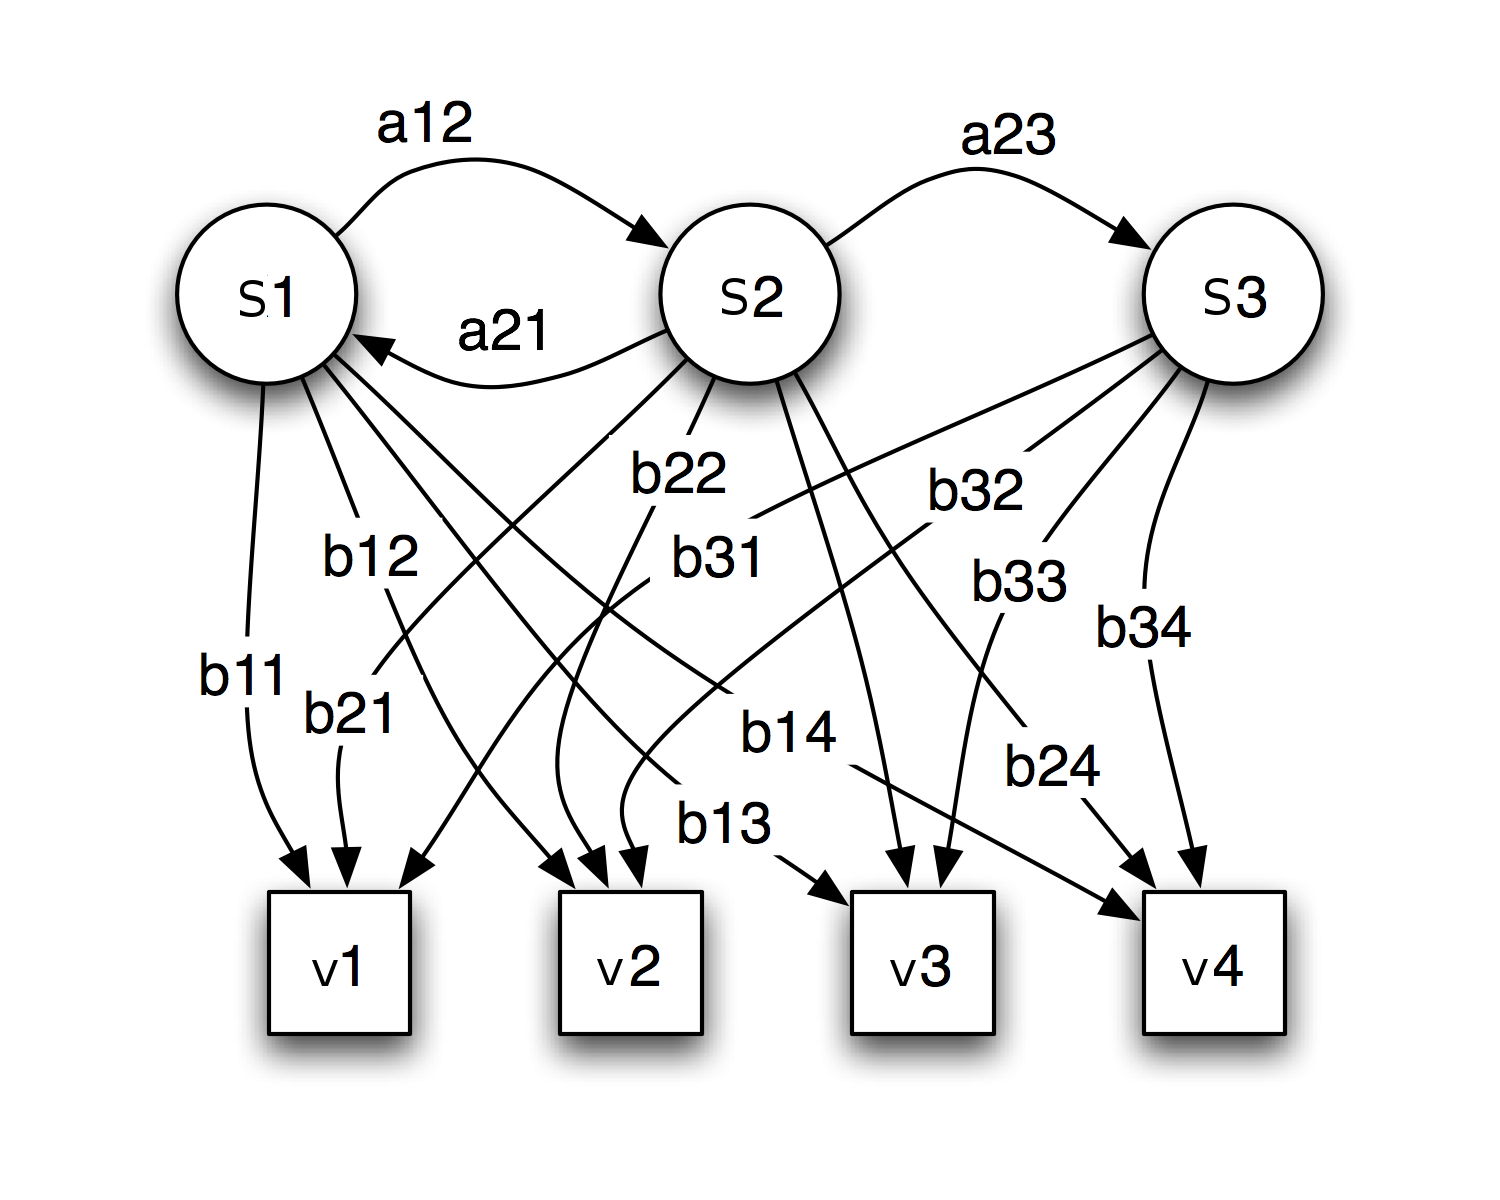
\includegraphics[width=0.8\textwidth]{./graphics/hmm.png}
\caption{Representaci\'on gr\'afica de un modelo oculto de Markov.}
\label{figure:hmm}
\end{figure}

\section[El Reconocimiento del Habla como Problema Estad{\'\i}stico]
{El Reconocimiento del Habla como Problema \\ Estad{\'\i}stico}

Para un lenguaje $L$ y una entrada ac\'ustica $X$, el problema del reconocimiento del habla puede definirse 
como \cite{Jurafsky}:

\begin{quote}
\emph{La b\'usqueda de la oraci\'on m\'as probable perteneciente al lenguaje L, dada la entrada ac\'ustica X.}
\end{quote}

La secuencia de observaciones ac\'usticas $O$ puede representarse como:

\begin{align}
O = o_1,o_2,o_3,\ldots,o_T\label{eq:asrO}
\end{align}

donde la se\~nal de voz fue dividida en $T$ muestras de igual duraci\'on.

La oraci\'on de salida, a su vez, puede representarse como:

\begin{align}
W  = w_1,w_2,w_3,\ldots,w_M\label{eq:asrW}
\end{align}

donde la cadena est\'a compuesta por $M$ palabras.

De esta manera, la definici\'on introducida anteriormente puede expresarse matem\'aticamente como:

\begin{align}
\hat{W} = \argmax_{W \in L} P(W|O)
\end{align}

Se escribe $\hat{W}$ por tratarse de una aproximaci\'on probabil{\'\i}stica.
Usando la Regla de Bayes la expresi\'on anterior puede reescribirse como:

\begin{align}
\hat{W} = \argmax_{W \in L} \frac{P(O|W)P(W)}{P(O)}
\end{align}

Como se desea obtener la oraci\'on con mayor probabilidad dada una entrada ac\'ustica, la entrada es
la misma para todas las oraciones evaluadas y su probabilidad de ocurrencia $P(O)$ se mantiene constante.
Puesto de otra manera, el t\'ermino $P(O)$ es independiente de $W$, por lo cual puede despreciarse. 

Por tanto:

\begin{align}
\hat{W} = \argmax_{W \in L} P(O|W)P(W)
\end{align}

El primer t\'ermino representa la probabilidad de una entrada ac\'ustica dada una secuencia de palabras, tambi\'en
conocida como verosimilitud de observaci\'on o modelo ac\'ustico. El segundo t\'ermino es la probabilidad 
\foreign{a priori} de ocurrencia de una secuencia de palabras, tambi\'en conocida como probabilidad previa o 
modelo de lenguaje. Esto es:

\begin{align}
\hat{W} = \argmax_{W \in L} \overbrace{P(O|W)}^\text{M. ac\'ustico}\overbrace{P(W)}^\text{M. de lenguaje}
\label{eq:asrFundamental}
\end{align}

Esta ecuaci\'on es el fundamento del enfoque estad{\'\i}stico al problema del reconocimiento del habla, base de los
sistemas \mbox{modernos \cite{RabinerStatistical2006}}.

\begin{figure}[H] 
\centering
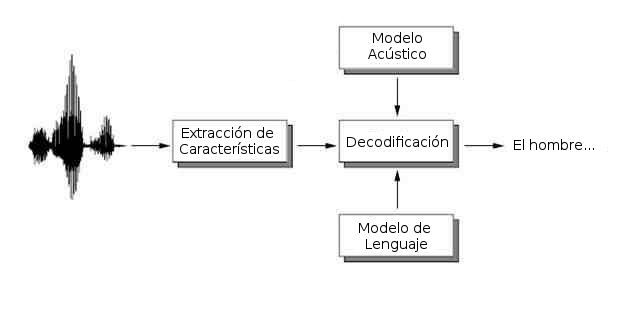
\includegraphics[width=0.8\textwidth]{./graphics/proceso.png}
\caption{Proceso b\'asico del reconocimiento del habla. Traducido a partir de \cite{VerenichASR}.}
\label{figure:proceso}
\end{figure}

La figura \ref{figure:proceso} ilustra de modo general la arquitectura de un sistema de reconocimiento del habla.
El proceso b\'asico del reconocimiento del habla, puede descomponerse en dos etapas o fases, cada una de las cuales
recibe una entrada (o varias) y produce una salida determinada.

\begin{itemize}
\item La primera fase o \emph{extracci\'on de caracter{\'\i}sticas} tiene como objetivo caracterizar la se\~nal
de voz para obtener una representaci\'on adecuada para el decodificador. Para tal efecto, produce vectores de
caracter{\'\i}sticas espectrales a partir del sonido que recibe como entrada.
\item La segunda fase o \emph{decodificaci\'on} tiene como objectivo producir la secuencia de palabras m\'as probable
dados los vectores de caracter{\'\i}sticas resultantes de la fase anterior. Para ello se sirve un modelo ac\'ustico, un
modelo de lenguaje y un algoritmo de decodificaci\'on.
\end{itemize}

Las siguientes secciones explican de manera m\'as detallada los conceptos y algoritmos relacionados a cada fase.
Tanto el modelo ac\'ustico como el modelo de lenguaje pueden requerir una fase de entrenamiento, 
previa a la utilizaci\'on del sistema de reconocimiento del habla.
Por motivos de claridad, los detalles de esta fase se presentan en \'ultimo lugar.

%!TEX root = ../tesis.tex
\subsection{Fase 1: Extracci\'on de caracter{\'\i}sticas}
\label{sec:featureExtraction}

En la primera fase, la entrada es la se\~nal de voz correspondiente al emisor, la cual se divide en muestras de corta
duraci\'on llamadas tramas. A trav\'es de un proceso de procesamiento de la onda sonora, se obtienen vectores de 
caracter{\'\i}sticas representativas para cada trama. Esta secci\'on describe los conceptos relacionados a esta 
transformaci\'on.

\subsubsection{Ondas Sonoras}

La entrada para un reconocedor del habla, y en particular para la fase 1, es la misma que la del o{\'\i}do humano: una 
serie de cambios en la presi\'on del aire \cite{YoungUniversity2007}. Estos cambios se originan en el emisor, y son 
causados por el aire que es expulsado de los pulmones, pasa por el tracto vocal y salen por la boca. As{\'\i}, para el 
proceso de s{\'\i}ntesis del habla en el ser humano, los pulmones son la fuente
del sonido y el trato vocal es el filtro que genera los distintos tipos de \mbox{sonido \cite{BradburyLineal2000}}.

Como mencionaba Semat ya en los a\~nos 50, existen dos aspectos del sonido: el f{\'\i}sico y el perceptual. De acuerdo al 
aspecto considerado, var{\'\i}an los t\'erminos con los cuales se describe al sonido; as{\'\i}, un f{\'\i}sico describe un 
sonido en t\'erminos de frecuencia, amplitud y n\'umero de sobretonos, mientras un m\'usico utiliza t\'erminos como tono, 
volumen o \mbox{timbre \cite{SematPhysics1958}}.

Aunque no existe una correspondencia directa entre las car\'acter{\'\i}sticas f{\'\i}sicas y las perceptuales 
\cite{SematPhysics1958}, existe una correlaci\'on en ciertos casos. As{\'\i}, para los sonidos con una frecuencia alta se 
percibe un tono m\'as agudo, aunque esta relaci\'on no es lineal. Igualmente, a mayor amplitud de una onda sonora esta se 
percibe con mayor \mbox{volumen \cite{YoungUniversity2007}}.

\subsubsection{Espectro}
El an\'alisis espectral est\'a basado en la conclusi\'on de Fourier que establece que una onda compleja puede ser 
representada como la sumatoria de varias ondas simples a diferentes frecuencias. El espectro es la representaci\'on de las 
distintas frecuencias que componen una onda, que puede visualizarse mediante una gr\'afica de amplitud en funci\'on de la 
\mbox{frecuencia \cite{Jurafsky}}. 

Los picos espectrales del espectro del sonido se conocen como formantes \cite{Fant1960acoustic}. Distinto fonemas poseen 
formantes a frecuencias determinadas, raz\'on por la cual el an\'alisis espectral tiene un rol determinante en la 
determinaci\'on de la identidad de vocales y otros \mbox{fonemas \cite{LadefogedCourse2006}}.

%Figura%

Un espectrograma, por su parte, es una matriz de celdas indexadas por frecuencia en el eje vertical y por tiempo en el eje 
horizontal, donde el nivel de sombreado de una celda indica la amplitud de la componente a una frecuencia y un tiempo 
dados. Aunque rara vez se use directamente para caracterizar la se\~nal, por resultar poco conveniente en t\'erminos del 
tama\~no de la representaci\'on, la gran mayor{\'\i}a de las caracter{\'\i}sticas utilizadas para el reconocimiento del 
habla est\'an basadas en el \mbox{espectrograma \cite{Ellis08anintroduction}}.

%Figura%

\subsubsection{Proceso de Extracci\'on de Caracter{\'\i}sticas}
El proceso puede resumirse en los siguientes pasos \cite{Jurafsky}:

\begin{enumerate}
\item \emph{Muestreo}: consiste en medir la amplitud de la se\~nal en un momento dado; la frecuencia de muestreo es el 
n\'umero de muestras que se toma por segundo. 

De acuerdo a la f\'ormula de Nyquist, es necesario que la frecuencia de muestreo sea al menos el doble de la frecuencia 
correspondiente a la onda que se desea medir. Por ejemplo, para las conversaciones telef\'onicas, cuyas frecuencias no 
superan los 4000 Hz, una frecuencia de muestreo de 8000 Hz resulta suficiente.

\item \emph{Cuantificaci\'on}: consiste en representar el n\'umero real correspondiente a la amplitud como un n\'umero entero, normalmente de 8
o 16 bits, para cada muestra. Con este paso finaliza la transformaci\'on de anal\'ogico a digital de la se\~nal de voz.

\item \emph{Conversi\'on}: una vez digitalizada, la se\~nal se convierte a un conjunto de caracter{\'\i}sticas espectrales. Los detalles de este 
paso dependen en gran medida del conjunto de caracter{\'\i}sticas que se selecciona para representar a la se\~nal.

\end{enumerate}

\subsubsection{Caracter{\'\i}sticas}
Un buen conjunto de caracter{\'\i}sticas re\'une las siguientes cualidades \cite{KesarkarFeature2003}:
\begin{itemize}
\item Las caracter{\'\i}sticas son perceptualmente significativas, es decir, an\'alogas a las utilizadas por el sistema 
auditivo humano.
\item Las caracter{\'\i}sticas son invariantes, es decir, robustas con respecto a las variaciones en el canal y el emisor.
\item Las caracter{\'\i}sticas capturan la din\'amica espectral, es decir, los cambios del espectro en el tiempo.
\end{itemize}

Algunos de los conjuntos de caracter{\'\i}sticas que se utilizan son:
\begin{itemize}
\item \emph{Codificaci\'on Predictiva Lineal (LPC)}: representaci\'on del espectro basada en la idea de que una muestra 
sonora puede ser aproximada mediante la combinaci\'on lineal de muestras \mbox{anteriores \cite{KesarkarFeature2003}}.
\item \emph{An\'alisis Cepstral en escala de Mel}: es el conjunto de caracter{\'\i}sticas m\'as com\'unmente utilizado. 
Basado en el concepto de ceptro, una representaci\'on que convierte los efectos del filtrado sobre una onda en una 
operaci\'on de adici\'on. Los coeficientes cesptrales se representan en la escala de Mel, una escala de frecuencia no
lineal de frecuencia basada en la percepci\'on de \mbox{tonos \cite{Ellis08anintroduction}}.
\item \emph{An\'alisis Predictivo Lineal Perceptual}: se basa en las caracter{\'\i}sticas LPC y las modifica de manera 
consistente a la percepci\'on por parte del ser humano. Por ejemplo, toma en cuenta los problemas de las personas para 
percibir ondas de alta frecuencia y la relaci\'on entre volumen e intensidad como factores para la transformaci\'on de las 
\mbox{caracter{\'\i}sticas \cite{Jurafsky}}. 
\end{itemize}

La evaluaci\'on y comparaci\'on de estos conjuntos de caracter{\'\i}sticas espectrales, de manera a determinar el m\'as 
indicado para el reconocimiento del habla, es tema de numerosos trabajos de 
\mbox{investigaci\'on \cite{DorraComparative2006, SarosiComparison2011, ElminirEvaluation2012}}.
%!TEX root = ../tesis.tex
\subsection{Fase 3: Decodificaci\'on}
\label{sec:decoding}

Durante este fase, se utiliza un algoritmo decodificador, que depende de un modelo de lenguaje y un diccionario de
pronunciaciones, para obtener la secuencia de palabras m\'as probable en base a las probabilidades que se calcularon 
anteriormente. Esta secci\'on describe los elementos involucrados en esta transformaci\'on, la cual constituye el paso
final del proceso simplificado del reconocimiento del habla que se pretende presentar.

\subsubsection{Modelos de Lenguaje}
Sea $V$ el conjunto finito de palabras que componen un lenguaje, tambi\'en conocido como vocabulario, y $V^\dag$ el 
conjunto infinito de oraciones que pueden formarse con palabras pertenecientes al vocabulario.

Un modelo de lenguaje \cite{CollinsLanguage} consiste en un conjunto finito $V$ y una funci\'on $p(x_1,x_2,\ldots,x_n)$ tal que:
\begin{enumerate}

\item $\forall (x_1,x_2,\ldots,x_n) \in V^\dag, p(x_1,x_2,\ldots,x_n) \ge 0$

\item $\displaystyle \sum_{(x_1,x_2,\ldots,x_n) \in V^\dag} p(x_1,x_2,\ldots,x_n) = 1$
\end{enumerate}

En resumen, un modelo de lenguaje busca predecir la probabilidad de una secuencia de palabras. 

La t\'ecnica predominante para construir modelos de lenguaje, debido a su simplicidad y efectividad, es la basada en 
n-gramas \cite{GaoComparative2010}. Sea $W^L_1$ una cadena de palabras pertenecientes a un vocabulario $V$ dado. Un modelo de 
lenguaje basado en n-gramas asigna la probabilidad a $W^L_1$ de acuerdo a:

\begin{equation*}
p(W^L_1) = \displaystyle \prod^L_{i = 1} w_i \mid w^{i - 1}_1 \approx \displaystyle \prod^L_{i = 1} w_i \mid w^{i - 1}_{i - n + 1}
\end{equation*}

Esta aproximaci\'on se basa en la suposici\'on de Markov de que cada palabra depende solo de las $n - 1$ palabras precedentes.

\subsubsection{Modelos Ocultos de Markov}
Un modelo oculto de Markov es un aut\'omata finito estoc\'astico entrenable \cite{KouemouHistory2011}, que implica un doble 
proceso estoc\'astico:

\begin{itemize}
\item El primer proceso, que produce una secuencia de estados, no es observable. Esto es, la secuencia de estados que produce
permanece oculta.
\item El segundo proceso produce una secuencia de observaciones, donde cada observaci\'on es una funci\'on probabil{\'\i}stica de un estado
correspondiente al primer proceso.
\end{itemize}

Un modelo oculto de Markov puede ser caracterizado mediante los siguientes elementos \cite{Rabiner89atutorial}:

\begin{enumerate}
\item $N$, el n\'umero de estados del modelo. Se representan los estados individuales como $S=\{S_1,S_2,\ldots,S_N\}$.
\item $M$, el n\'umero de s{\'\i}mbolos observables por estado. Se representan los s{\'\i}mbolos individuales como $V=\{v_1,v_2,\ldots,v_M\}$
\item La distribuci\'on de probabilidad de transici\'on de estados $A = \left\{a_ij\right\}$, donde:
\begin{align*}
	a_ij = P[q_{t+1} = S_j \mid q_t = S_i], & & 1 \leq i,j & \leq N
\end{align*}
\item La distribuci\'on de probabilidad de los s{\'\i}mbolos observables en el estado $j$, $b_j(k)$, tambi\'en representada como $b_j(v_k)$, 
donde:
\begin{align*}
	b_j(v_k) = P[v_k \text{ en el momento } t \mid q_t = S_j], & & 1 \leq j & \leq N
	\\& & 1 \leq k & \leq M
\end{align*}
\item La distribuci\'on de probabilidad del estado inicial $\pi=\left\{\pi_i\right\}$, donde:
\begin{align*}
	\pi_i = P[q_1=S_i], & & 1 \leq i \leq N
\end{align*}
\end{enumerate}

De modo a comprender mejor este concepto que puede resultar complejo, se presenta a continuaci\'on un ejemplo cl\'asico de un modelo oculto de
Markov. El ejemplo se denomina \emph{El modelo de la urna y la pelota} \cite{Rabiner89atutorial}:

\begin{quote}
	Se asume que hay N urnas (grandes) de vidrio en una habitaci\'on. Dentro de cada urna hay un gran n\'umero de pelotas de colores.
	Un genio est\'a en la habitaci\'on y, de acuerdo a un proceso aleatorio, elige una urna inicial. De esta urna extrae una pelota de
	manera aleatoria y su color se anota como la observaci\'on, pues el observador desconoce la urna de donde sali\'o la pelota.
	La pelota se coloca de nuevo en la urna y se repiten la selecci\'on de la urna y la pelota respectivamente. Este proceso genera
	una secuencia aleatoria de colores.
\end{quote}

Este sencillo sistema puede modelarse como un modelo oculto de Markov con los siguientes par\'ametros:
\begin{enumerate}
	\item $N$ es el n\'umero de urnas.
	\item $M$ es la cantidad de colores posibles de las pelotas en las urnas.
	\item $A$ es la funci\'on que determina la transici\'on entre urnas.
	\item $b_j(v_k)$ es la funci\'on que determina la elecci\'on de una pelota de determinado color.
	\item $\pi$ es la funci\'on que determina la elecci\'on de la urna inicial.
\end{enumerate}

\subsubsection{Algoritmo de Viterbi}
El algoritmo de Viterbi recibe una secuencia de observaciones y un \'unico aut\'omata y retorna el camino \'optimo a trav\'es
del aut\'omata, esto es, la mejor secuencia de estados. La descipci\'on y el pseudoc\'odigo que se presentan en esta secci\'on
est\'an basados principalmente en \cite{Jurafsky, Rabiner89atutorial}.

M\'as formalmente, se busca la mejor secuencia de estados $Q = (q_1,q_2,\ldots,q_T)$ dadas una secuencia de observaciones
$O = (o_1,o_2,\ldots,o_T)$ y un modelo $\lambda$.

El algoritmo utiliza una matriz de probabilidades $viterbi$, donde cada celda $viterbi[i,t]$ contiene la probabilidad del
mejor camino teniendo en cuenta las $t$ primeras observaciones y terminando en el estado $i$ del modelo. Esto es:

\begin{equation*}
	viterbi[i,t] = \displaystyle \max_{q_1,q_2,\ldots,q_{t - 1}} P(q1,q2,\ldots,q_{t - 1},q_t = i,o_1,o_2,\ldots,o_t \mid \lambda) 	
\end{equation*} 

Para calcular los valores de $viterbi[i,t]$, el algoritmo de Viterbi asume la invariante de la programaci\'on din\'amica.
Esto es, se asume que si el mejor camino para una secuencia de observaciones pasa por un estado $q_i$, entonces este
camino incluye el mejor camino hasta $q_i$ inclusive. Este supuesto, aunque no siempre sea correcto, permite descomponer
el problema y simplificar su soluci\'on, mediante la siguiente relaci\'on de recurrencia:

\begin{equation*}
	viterbi[i,t] = \displaystyle \max_i (viterbi[i,t-1]a_{i,j})b_j(o_t)
\end{equation*}

\begin{algorithm}[H]
\caption{Algoritmo de Viterbi} \label{viterbi}
\begin{algorithmic}[1]
\REQUIRE $observaciones$ de longitud $T$, $grafo\mbox{-}estados$.
\ENSURE $estados$, el mejor camino.
\STATE $num\mbox{-}estados \leftarrow$ CANTIDAD-DE-ESTADOS($grafo\mbox{-}estados$) 
\STATE Crear una matriz de probabilidades $viterbi[num\mbox{-}estados, T]$
\FOR{cada estado $s$ desde $0$ hasta $num\mbox{-}estados$}
	\STATE $viterbi[s,0] = \pi_s$
\ENDFOR
\FOR{cada paso $t$ desde $0$ hasta $T - 1$}
	\FOR{cada estado $s$ desde $0$ hasta $num\mbox{-}estados$}
		\FOR{cada transici\'on $s$ desde s especificada por el $grafo\mbox{-}estados$}
		\STATE $nuevo\mbox{-}puntaje \leftarrow viterbi[s,t] * a[s,s'] * b_{s'}[o_t]$
		\IF{$viterbi[s',t+1] = 0 \parallel nuevo\mbox{-}puntaje > viterbi[s',t+1]$}
			\STATE $viterbi[s',t+1] \leftarrow nuevo\mbox{-}puntaje$
			\STATE $puntero\mbox{-}retroceso[s',t+1] \leftarrow s$
		\ENDIF  
		\ENDFOR
	\ENDFOR
\ENDFOR
\STATE $estados \leftarrow$ retroceso desde la celda con mayor valor en la \'ultima columna de $viterbi[]$
\\ \COMMENT{Usando $puntero-retroceso$}.
\RETURN $estados$
\end{algorithmic}
\end{algorithm}

\emph{Limitaciones del Algoritmo}

El algoritmo de Viterbi presenta dos limitaciones principales:
\begin{enumerate}
	\item No retorna la secuencia m\'as probable de palabras, sino la secuencia m\'as probable de estados. Aunque en muchos casos resulta casi
	equivalente, esto puede ser un problema para lenguajes en los cuales una misma palabra puede tener diferentes pronunciaciones.
	\item La invariante de la programaci\'on din\'amica, base del algoritmo, no es v\'alida para modelos de lenguaje m\'as complejos que una
	gram\'atica basada en bi-gramas.
\end{enumerate}

Existen dos clases de soluciones a estas limitaciones:
\begin{enumerate}
	\item Modificar el algoritmo de Viterbi de forma que retorne las $N$ oraciones m\'as probables como una lista, o como 
	rejillas (\foreign{lattices}) de palabras. Estas oraciones luego se reordenan usando un mejor modelo ac\'ustico o de lenguaje,
	de modo a seleccionar la oraci\'on m\'as probable.
	\item Utilizar otro algoritmo para la decodificaci\'on. La alternativa m\'as com\'un es el algoritmo decodificador de pila o A*, el cual
	se presenta a continuaci\'on.
\end{enumerate}

\subsubsection{Algoritmo A*}
El algoritmo de pila o A* es un algoritmo de b\'usqueda mejor-primero sobre un \'arbol, no representado expl{\'\i}citamente, que define las
secuencias de palabras aceptables en un lenguaje dado. La descipci\'on y el pseudoc\'odigo que se presentan en esta secci\'on
est\'an basados principalmente en \cite{Jurafsky, PaulEfficient1992}.

El \'arbol mencionado tiene palabras por nodos y cada hoja define una oraci\'on aceptada por el lenguaje, la que se forma concatenando las 
palabras desde la ra{\'\i}z hasta la hoja.  

El algoritmo mantiene una cola de prioridad, a la cual se denomina pila (de ah{\'\i} el otro nombre del algoritmo) \cite{PostStack}, 
de caminos o soluciones parciales, cada una asociada a un puntaje dado. La operaci\'on \foreign{pop} de la cola retorna el elemento 
con el puntaje m\'as alto. El puntaje de un elemento $p$ est\'a dado por la \mbox{funci\'on \cite{Jurafsky, Russell2003Solving}}:

\begin{equation*}
	f*(p) = g(p) + h*(p)
\end{equation*}

Donde $f*(p)$ es el puntaje estimado del mejor camino (oraci\'on completa) y est\'a dado por:

\begin{itemize}
 	\item $g(p)$, el puntaje del camino parcial $p$. Esta funci\'on puede ser estimada por la probabilidad de $p$ dada la entrada ac\'ustica
 	hasta ese momento. Esto es, $P(X \mid W)P(W)$ para la secuencia de palabras $W$ que constituye $p$. 

 	Esta probabilidad se calcula usando el algoritmo de Avance, una alternativa menos eficiente para m\'as precisa al algoritmo de 
 	\mbox{Viterbi \cite{Jurafsky}}.

 	\item $h*(p)$, una estimaci\'on del puntaje de la mejor extensi\'on de $p$ hasta el final del camino. La estimaci\'on de $h*$ es un problema
 	no resuelto e interesante. 

 	Un enfoque posible es elegir como $h*$ una estimaci\'on relacionada al n\'umero de palabras que faltan para
 	completar la oraci\'on.
 \end{itemize}

 Luego de seleccionar un camino parcial, se utiliza un algoritmo de b\'usqueda r\'apida para encontrar palabras candidatas para extender
 la soluci\'on parcial. Varios algoritmos de b\'usqueda \cite{GuptaFast1988, BahlSpeech1993} r\'apida se basan en la utilizaci\'on de un 
 \'arbol l\'exico \cite{KlovstadCasper1975}, el cual almacena las pronunciaciones de todas las palabras de forma que el c\'omputo de la 
 probabilidad puede ser compartido entre palabras de similar pronunaciaci\'on.

Las oraciones extendidas vuelven a insertarse en la cola, y el proceso se repite hasta procesar toda la entrada ac\'ustica.

\begin{algorithm}[H]
	\caption{Algoritmo A*} \label{stack}
\begin{algorithmic}[1]
	\STATE Inicializar la cola de prioridad con una teor{\'\i}a nula.
	\STATE Hacer \foreign{pop}, obteniendo la teor{\'\i}a $s$ con mejor puntaje de la cola.
	\WHILE{! $bandera\mbox{-}FDO$ de $s$}
		\STATE Hacer una b\'usqueda r\'apida para obtener palabras candidatas para extender $s$.
		\FOR{cada palabra $w$ en la lista de candidatos}
			\STATE Construir una nueva oraci\'on candidata $s + w$.
			\STATE Usar el algoritmo de Avance para calcular $P(X \mid s + w) \rightarrow L$
			\STATE Usar el modelo de lenguaje para calcular $P(W) \rightarrow P$
			\STATE Calcular el puntaje de $s + w$ mediante una funci\'on de $L, P$ y $h^*$
			\IF{fin-de-oracion}
				\STATE $bandera\mbox{-}FDO$ de $s \leftarrow verdadero$
			\ENDIF
			\STATE Insertar $s + w$ con su puntaje y $bandera\mbox{-}FDO$ a la cola de prioridad.
			\STATE Hacer \foreign{pop}, obteniendo la teor{\'\i}a $s$ con mejor puntaje de la cola.
		\ENDFOR
	\ENDWHILE
\end{algorithmic}
\end{algorithm}
%!TEX root = ../tesis.tex
\section{Fase Previa: Entrenamiento}
\label{sec:training}

El proceso b\'asico que se describi\'o en las secciones anteriores requiere de modelos probabil{\'\i}sticos para
solucionar el problema del reconocimiento del habla. Para definir estos modelos es necesaria una
fase previa de entrenamiento, durante la cual se utilizan corpus de sonido y texto, denominados tambi\'en
como datos de entrenamiento.

\subsection{Modelo de Lenguaje}

Para entrenar un modelo de lenguaje basado en n-gramas es necesario un corpus de texto que 
sirva de ejemplo del lenguaje que busca reconocerse.

El modelo se entrena contando las ocurrencias de cada n-grama en el corpus de texto, para luego
normalizar el conteo dividiendo sobre la cantidad total de n-gramas en el corpus.
A continuaci\'on se utilizan normalmente m\'etodos de reestimaci\'on, de modo a mejorar las estimaciones 
de n-gramas con un conteo muy bajo, o incluso igual a cero. Este proceso se conoce como suavizamiento
del modelo.

Finalmente, el conteo normalizado y suavizado de cada n-grama en el corpus del texto constituye su
probabilidad \cite{CollinsLanguage}.

Un modelo de lenguaje basado en gram\'aticas no requiere de entrenamiento previo, por lo cual puede
utilizarse en casos en los cuales no se disponga de un corpus de texto de tama\~no suficiente.
A\'un as{\'\i}, si se dispone de datos de entrenamiento, es posible incluir las probabilidades estimadas
a partir del corpus en la gram\'atica \cite{huang-handbook10}.

\subsection{HMM: Estructura del grafo de estados}
El conjunto de estados de cada \gls{hmm}, $S$, y las transiciones entre estos estados se definen en base
al diccionario fon\'etico. A modo de ejemplo, \mbox{CMUDdict \cite{CMUdict}} es un diccionario fon\'etico
que contiene correspondencias entre palabras y las secuencias de fonemas que las componen para m\'as de
125.000 palabras del idioma ingl\'es.

\begin{figure}[H]
\begin{lstlisting}
HOUSE  HH AW1 S
HOUSE'S  HH AW1 S IH0 Z
HOUSEAL  HH AW1 S AH0 L
HOUSEBOAT  HH AW1 S B OW2 T
HOUSEBOATS  HH AW1 S B OW2 T S
HOUSEBROKEN  HH AW1 S B R OW2 K AH0 N
HOUSECLEANING  HH AW1 S K L IY2 N IH0 NG
HOUSED  HH AW1 Z D
HOUSEFUL  HH AW1 S F AH0 L
HOUSEGUEST  HH AW1 S G EH0 S T
\end{lstlisting}
\caption{Extracto del diccionario fon\'etico CMUdict \cite{CMUdict}.}
\end{figure}

\subsection{HMM: Distribuciones de Probabilidad}
Para cada \gls{hmm} es necesario estimar los siguientes par\'ametros, definidos en la secci\'on \ref{sec:hmm}:
	\begin{itemize}
		\item Las probabilidades de estado inicial: $\pi_i$
		\item Las probabilidades de transici\'on: $a_{ij}$
		\item Las probabilidades de observaci\'on: $b_j(o_t)$ 
	\end{itemize}

Para esto se cuenta con \cite{Jurafsky}:
	\begin{itemize}
		\item  Un corpus de voz, compuesto por una colecci\'on de grabaciones de voz junto
		con sus transcripciones de texto.
		\item Un corpus de voz de menor tama\~no etiquetado fon\'eticamente. 
		Esto es, donde fragmentos de la se\~nal est\'an asociados a su fonema correspondiente.
	\end{itemize}

La primera etapa del entrenamiento consiste en una estimaci\'on inicial de los par\'ametros en base a los
datos de entrenamiento.

Para las probabilidades de estado inicial, se asume que cualquier estado es igualmente probable 
como estado inicial. De manera similar, para las probabilidades de transici\'on se asume que, para cada estado, cualquier transici\'on a otro estado es igualmente probable.

Las probabilidades de observaci\'on se estiman inicialmente mediante el peque\~no corpus 
de voz etiquetado fon\'eticamente.

La siguiente etapa var{\'\i}a de acuerdo al m\'etodo escogido para la definici\'on de las probabilidades
de observaci\'on, $b_j$. Si se utilizan funciones Gaussianas, el cual constituye el caso m\'as
frecuente, las estimaciones iniciales se mejoran mediante el algoritmo de Baum--Welch.

El algoritmo de Baum--Welch calcula dos probabilidades adicionales en base a las estimaciones
iniciales de $a_{ij}$ y $b_j(o_t)$, denominadas probabilidad de avance y probabilidad de retroceso. 
Utilizando estas probabilidades, se mejoran las estimaciones $a_{ij}$ y $b_j(o_t)$ mediante
un proceso iterativo que se repite hasta que los valores converjan \cite{Rabiner89atutorial}.
%!TEX root = ../tesis.tex
\subsection{Fase 1: Extracci\'on de caracter{\'\i}sticas}
\label{sec:featureExtraction}

En la primera fase, la entrada es la se\~nal de voz correspondiente al emisor, la cual se divide en muestras de corta
duraci\'on llamadas tramas. A trav\'es de un proceso de procesamiento de la onda sonora, se obtienen vectores de 
caracter{\'\i}sticas representativas para cada trama. Esta secci\'on describe los conceptos relacionados a esta 
transformaci\'on.

\subsubsection{Ondas Sonoras}

La entrada para un reconocedor del habla, y en particular para la fase 1, es la misma que la del o{\'\i}do humano: una 
serie de cambios en la presi\'on del aire \cite{YoungUniversity2007}. Estos cambios se originan en el emisor, y son 
causados por el aire que es expulsado de los pulmones, pasa por el tracto vocal y salen por la boca. As{\'\i}, para el 
proceso de s{\'\i}ntesis del habla en el ser humano, los pulmones son la fuente
del sonido y el trato vocal es el filtro que genera los distintos tipos de \mbox{sonido \cite{BradburyLineal2000}}.

Como mencionaba Semat ya en los a\~nos 50, existen dos aspectos del sonido: el f{\'\i}sico y el perceptual. De acuerdo al 
aspecto considerado, var{\'\i}an los t\'erminos con los cuales se describe al sonido; as{\'\i}, un f{\'\i}sico describe un 
sonido en t\'erminos de frecuencia, amplitud y n\'umero de sobretonos, mientras un m\'usico utiliza t\'erminos como tono, 
volumen o \mbox{timbre \cite{SematPhysics1958}}.

Aunque no existe una correspondencia directa entre las car\'acter{\'\i}sticas f{\'\i}sicas y las perceptuales 
\cite{SematPhysics1958}, existe una correlaci\'on en ciertos casos. As{\'\i}, para los sonidos con una frecuencia alta se 
percibe un tono m\'as agudo, aunque esta relaci\'on no es lineal. Igualmente, a mayor amplitud de una onda sonora esta se 
percibe con mayor \mbox{volumen \cite{YoungUniversity2007}}.

\subsubsection{Espectro}
El an\'alisis espectral est\'a basado en la conclusi\'on de Fourier que establece que una onda compleja puede ser 
representada como la sumatoria de varias ondas simples a diferentes frecuencias. El espectro es la representaci\'on de las 
distintas frecuencias que componen una onda, que puede visualizarse mediante una gr\'afica de amplitud en funci\'on de la 
\mbox{frecuencia \cite{Jurafsky}}. 

Los picos espectrales del espectro del sonido se conocen como formantes \cite{Fant1960acoustic}. Distinto fonemas poseen 
formantes a frecuencias determinadas, raz\'on por la cual el an\'alisis espectral tiene un rol determinante en la 
determinaci\'on de la identidad de vocales y otros \mbox{fonemas \cite{LadefogedCourse2006}}.

%Figura%

Un espectrograma, por su parte, es una matriz de celdas indexadas por frecuencia en el eje vertical y por tiempo en el eje 
horizontal, donde el nivel de sombreado de una celda indica la amplitud de la componente a una frecuencia y un tiempo 
dados. Aunque rara vez se use directamente para caracterizar la se\~nal, por resultar poco conveniente en t\'erminos del 
tama\~no de la representaci\'on, la gran mayor{\'\i}a de las caracter{\'\i}sticas utilizadas para el reconocimiento del 
habla est\'an basadas en el \mbox{espectrograma \cite{Ellis08anintroduction}}.

%Figura%

\subsubsection{Proceso de Extracci\'on de Caracter{\'\i}sticas}
El proceso puede resumirse en los siguientes pasos \cite{Jurafsky}:

\begin{enumerate}
\item \emph{Muestreo}: consiste en medir la amplitud de la se\~nal en un momento dado; la frecuencia de muestreo es el 
n\'umero de muestras que se toma por segundo. 

De acuerdo a la f\'ormula de Nyquist, es necesario que la frecuencia de muestreo sea al menos el doble de la frecuencia 
correspondiente a la onda que se desea medir. Por ejemplo, para las conversaciones telef\'onicas, cuyas frecuencias no 
superan los 4000 Hz, una frecuencia de muestreo de 8000 Hz resulta suficiente.

\item \emph{Cuantificaci\'on}: consiste en representar el n\'umero real correspondiente a la amplitud como un n\'umero entero, normalmente de 8
o 16 bits, para cada muestra. Con este paso finaliza la transformaci\'on de anal\'ogico a digital de la se\~nal de voz.

\item \emph{Conversi\'on}: una vez digitalizada, la se\~nal se convierte a un conjunto de caracter{\'\i}sticas espectrales. Los detalles de este 
paso dependen en gran medida del conjunto de caracter{\'\i}sticas que se selecciona para representar a la se\~nal.

\end{enumerate}

\subsubsection{Caracter{\'\i}sticas}
Un buen conjunto de caracter{\'\i}sticas re\'une las siguientes cualidades \cite{KesarkarFeature2003}:
\begin{itemize}
\item Las caracter{\'\i}sticas son perceptualmente significativas, es decir, an\'alogas a las utilizadas por el sistema 
auditivo humano.
\item Las caracter{\'\i}sticas son invariantes, es decir, robustas con respecto a las variaciones en el canal y el emisor.
\item Las caracter{\'\i}sticas capturan la din\'amica espectral, es decir, los cambios del espectro en el tiempo.
\end{itemize}

Algunos de los conjuntos de caracter{\'\i}sticas que se utilizan son:
\begin{itemize}
\item \emph{Codificaci\'on Predictiva Lineal (LPC)}: representaci\'on del espectro basada en la idea de que una muestra 
sonora puede ser aproximada mediante la combinaci\'on lineal de muestras \mbox{anteriores \cite{KesarkarFeature2003}}.
\item \emph{An\'alisis Cepstral en escala de Mel}: es el conjunto de caracter{\'\i}sticas m\'as com\'unmente utilizado. 
Basado en el concepto de ceptro, una representaci\'on que convierte los efectos del filtrado sobre una onda en una 
operaci\'on de adici\'on. Los coeficientes cesptrales se representan en la escala de Mel, una escala de frecuencia no
lineal de frecuencia basada en la percepci\'on de \mbox{tonos \cite{Ellis08anintroduction}}.
\item \emph{An\'alisis Predictivo Lineal Perceptual}: se basa en las caracter{\'\i}sticas LPC y las modifica de manera 
consistente a la percepci\'on por parte del ser humano. Por ejemplo, toma en cuenta los problemas de las personas para 
percibir ondas de alta frecuencia y la relaci\'on entre volumen e intensidad como factores para la transformaci\'on de las 
\mbox{caracter{\'\i}sticas \cite{Jurafsky}}. 
\end{itemize}

La evaluaci\'on y comparaci\'on de estos conjuntos de caracter{\'\i}sticas espectrales, de manera a determinar el m\'as 
indicado para el reconocimiento del habla, es tema de numerosos trabajos de 
\mbox{investigaci\'on \cite{DorraComparative2006, SarosiComparison2011, ElminirEvaluation2012}}.
\subsection{Fase 2: Estimaci\'{o}n de Verosimilitud de Fonemas}
\label{sec:phoneLikelihood}

La fase anterior genera unos vectores de caracter\'{i}sticas que representan la se\~{n}al de voz. En esta secci\'{o}n
se muestra c\'{o}mo transformar estos vectores en probabilidades utilizando una funci\'on de densidad
de probabilidad.

\subsubsection{Funci\'on de Densidad de Probabilidad}
\label{sec:pdfs}

La salida de los m\'etodos descritos en esta secci\'on es una funci\'on de densidad de probabilidad (o PDF por sus siglas en 
ingl\'es). \'Esta es una funci\'on de destribuci\'on de probabilidades que permite mapear los vectores de 
caracter\'isticas a una probabilidad. Formalmente, permite estimar (utilizando un enfoque discreto o cont\'inuo)
la verosimilitud de la observaci\'on representada como $b_j(o_t)$.

\subsubsection{Cuantificaci\'{o}n Vectorial}
\label{sec:vectorQuantization}

La Cuantificac\'{o}n Vectorial permite modelar una PDF sobre un espacio discreto, agrupando a los vectores de caracter\'{i}sticas en 
s\'{i}mbolos discretos que pueden contarse. Luego calcula la probabilidad de un grupo contando la cantidad de veces 
que \'{e}ste ocurre dentro de un conjunto de entrenamiento.

Este m\'{e}todo era bastante utilizado en los primeros sistemas de reconocimiento del habla \cite{Jurafsky}, pero ha sido reemplazado
por t\'{e}cnicas de computo intensivo sobre un espacio cont\'{i}nuo en vez de uno discreto.

\subsubsection{M\'etodo Gaussiano}
\label{sec:gaussianPdf}
El m\'{e}todo Gaussiano es el m\'{a}s utilizado del enfoque cont\'{i}nuo. En su versi\'{o}n m\'{a}s simple, cada estado tiene
asociada una funci\'{o}n gaussiana que mapea el vector de observaciones $o_t$ a una probabilidad.

La versi\'{o}n simple del m\'etodo Gaussiano asume que los valores del vector de observaciones $o_t$ presentan una distribuci\'on
normal. Por lo tanto, la funci\'on de probabilidad de las observaciones, $b_j(o_t)$, se representa como una curva gaussiana con
media $\mu_j$ y matriz de covarianza $\Sigma_j$, calculadas mediante el algoritmo de Avance-Retroceso. Sin entrar en detalles 
matem\'aticos, se presenta la ecuaci\'on para calcular $b_j(o_t)$:

\begin{equation}
    b_j(o_t) = \frac{1}{\sqrt{(2\pi)|\Sigma_j|}}e^{[(o_t-\mu_j)'\Sigma_j^{-1}(o_t-\mu_j)]}
\end{equation}

En la pr\'actica la matriz $\Sigma_j$ es diagonal, lo que quiere decir que solo mantiene una media y varianza por cada vector
de caracter\'isticas.

Jurafsky en \cite{Jurafsky} menciona que la mayor\'ia sistemas actuales de reconocimiento del habla utilizan m\'ultiples funciones gaussianas 
para cada estado, de manera que la probabilidad se calcula como una combinaci\'on de estas funciones, t\'ecnica conocida como
Mezcla Gaussiana. Adem\'as, algunos sistemas comparten funciones gaussianas entre estados, t\'ecnica conocida como atadura de
par\'ametros. Algunos fonemas ac\'usticamente similares, por ejemplo, podr\'ian compartir funciones gaussianas.

\subsubsection{Redes Neuronales}
\label{sec:likelihoodNeuralNet}

Otro m\'etodo popularmente utilizado para modelar una PDF sobre un espacio cont\'inuo, es el que utiliza Redes Neuronales. 
De manera simplificada, una Red Neuronal es un conjunto de unidades computacionales unidas por enlazes ponderados. La red recibe
como entrada un vector de valores y retorna como salida otro vector de valores.

Este enfoque utiliza elementos del HMM (por ejemplo, el grafo que representa la pronunciaci\'on de una palabra) y un Perceptr\'on
Multicapa (o MLP por sus siglas en ingl\'es) para calcular la probabilidad de las observaciones, por eso a este m\'etodo se lo
conoce com\'unmente como enfoque H\'ibrido HMM-MLP. La entrada a esta red es un vector de caracter\'isticas en un tiempo $t$ y
otros vectores adicionales. Para que la red pueda utilizarse para computar la probabilidad de un estado $j$ dado un vector
de observaci\'ion $o_t$, formalmente $P(j|o_t)$, debe establecerse como restricci\'on que todas las unidades de salida sumen 1.

El MLP calcula la probabilidad $P(q_j|o_t)$ pero la probabilidad $b_j(o_t)$ que se busca es $P(o_t|q_j)$. Utilizando el teorema de
Bayes se puede obtener la probabilidad deseada a partir de la computada por el MLP:

\begin{equation}
    p(q_j|o_t) = \frac{P(o_t|q_j)p(q_j)}{p(o_t)}
\end{equation}

Acomodando los t\'erminos se obtiene:

\begin{equation}
    \frac{p(o_t|q_j)}{p(o_t)} = \frac{P(q_j|o_t)}{p(q_j)}
\label{eq:bayes-rea}
\end{equation}

Utilizando la ecuaci\'on \eqref{eq:bayes-rea} se puede computar $\frac{p(o_t|q_j)}{p(o_t)}$ denominada verosimilitud escalada. Esta
verosimilitud escalada es igual de buena que la verosimilitud com\'un \cite{Jurafsky}, ya que la probabilidad $p(o_t)$ es constante
durante el reconocimiento. De este modo, se obtiene la probabilidad $b_j(o_t)$ deseada.


%!TEX root = ../tesis.tex
\subsection{Fase 3: Decodificaci\'on}
\label{sec:decoding}

Durante este fase, se utiliza un algoritmo decodificador, que depende de un modelo de lenguaje y un diccionario de
pronunciaciones, para obtener la secuencia de palabras m\'as probable en base a las probabilidades que se calcularon 
anteriormente. Esta secci\'on describe los elementos involucrados en esta transformaci\'on, la cual constituye el paso
final del proceso simplificado del reconocimiento del habla que se pretende presentar.

\subsubsection{Modelos de Lenguaje}
Sea $V$ el conjunto finito de palabras que componen un lenguaje, tambi\'en conocido como vocabulario, y $V^\dag$ el 
conjunto infinito de oraciones que pueden formarse con palabras pertenecientes al vocabulario.

Un modelo de lenguaje \cite{CollinsLanguage} consiste en un conjunto finito $V$ y una funci\'on $p(x_1,x_2,\ldots,x_n)$ tal que:
\begin{enumerate}

\item $\forall (x_1,x_2,\ldots,x_n) \in V^\dag, p(x_1,x_2,\ldots,x_n) \ge 0$

\item $\displaystyle \sum_{(x_1,x_2,\ldots,x_n) \in V^\dag} p(x_1,x_2,\ldots,x_n) = 1$
\end{enumerate}

En resumen, un modelo de lenguaje busca predecir la probabilidad de una secuencia de palabras. 

La t\'ecnica predominante para construir modelos de lenguaje, debido a su simplicidad y efectividad, es la basada en 
n-gramas \cite{GaoComparative2010}. Sea $W^L_1$ una cadena de palabras pertenecientes a un vocabulario $V$ dado. Un modelo de 
lenguaje basado en n-gramas asigna la probabilidad a $W^L_1$ de acuerdo a:

\begin{equation*}
p(W^L_1) = \displaystyle \prod^L_{i = 1} w_i \mid w^{i - 1}_1 \approx \displaystyle \prod^L_{i = 1} w_i \mid w^{i - 1}_{i - n + 1}
\end{equation*}

Esta aproximaci\'on se basa en la suposici\'on de Markov de que cada palabra depende solo de las $n - 1$ palabras precedentes.

\subsubsection{Modelos Ocultos de Markov}
Un modelo oculto de Markov es un aut\'omata finito estoc\'astico entrenable \cite{KouemouHistory2011}, que implica un doble 
proceso estoc\'astico:

\begin{itemize}
\item El primer proceso, que produce una secuencia de estados, no es observable. Esto es, la secuencia de estados que produce
permanece oculta.
\item El segundo proceso produce una secuencia de observaciones, donde cada observaci\'on es una funci\'on probabil{\'\i}stica de un estado
correspondiente al primer proceso.
\end{itemize}

Un modelo oculto de Markov puede ser caracterizado mediante los siguientes elementos \cite{Rabiner89atutorial}:

\begin{enumerate}
\item $N$, el n\'umero de estados del modelo. Se representan los estados individuales como $S=\{S_1,S_2,\ldots,S_N\}$.
\item $M$, el n\'umero de s{\'\i}mbolos observables por estado. Se representan los s{\'\i}mbolos individuales como $V=\{v_1,v_2,\ldots,v_M\}$
\item La distribuci\'on de probabilidad de transici\'on de estados $A = \left\{a_ij\right\}$, donde:
\begin{align*}
	a_ij = P[q_{t+1} = S_j \mid q_t = S_i], & & 1 \leq i,j & \leq N
\end{align*}
\item La distribuci\'on de probabilidad de los s{\'\i}mbolos observables en el estado $j$, $b_j(k)$, tambi\'en representada como $b_j(v_k)$, 
donde:
\begin{align*}
	b_j(v_k) = P[v_k \text{ en el momento } t \mid q_t = S_j], & & 1 \leq j & \leq N
	\\& & 1 \leq k & \leq M
\end{align*}
\item La distribuci\'on de probabilidad del estado inicial $\pi=\left\{\pi_i\right\}$, donde:
\begin{align*}
	\pi_i = P[q_1=S_i], & & 1 \leq i \leq N
\end{align*}
\end{enumerate}

De modo a comprender mejor este concepto que puede resultar complejo, se presenta a continuaci\'on un ejemplo cl\'asico de un modelo oculto de
Markov. El ejemplo se denomina \emph{El modelo de la urna y la pelota} \cite{Rabiner89atutorial}:

\begin{quote}
	Se asume que hay N urnas (grandes) de vidrio en una habitaci\'on. Dentro de cada urna hay un gran n\'umero de pelotas de colores.
	Un genio est\'a en la habitaci\'on y, de acuerdo a un proceso aleatorio, elige una urna inicial. De esta urna extrae una pelota de
	manera aleatoria y su color se anota como la observaci\'on, pues el observador desconoce la urna de donde sali\'o la pelota.
	La pelota se coloca de nuevo en la urna y se repiten la selecci\'on de la urna y la pelota respectivamente. Este proceso genera
	una secuencia aleatoria de colores.
\end{quote}

Este sencillo sistema puede modelarse como un modelo oculto de Markov con los siguientes par\'ametros:
\begin{enumerate}
	\item $N$ es el n\'umero de urnas.
	\item $M$ es la cantidad de colores posibles de las pelotas en las urnas.
	\item $A$ es la funci\'on que determina la transici\'on entre urnas.
	\item $b_j(v_k)$ es la funci\'on que determina la elecci\'on de una pelota de determinado color.
	\item $\pi$ es la funci\'on que determina la elecci\'on de la urna inicial.
\end{enumerate}

\subsubsection{Algoritmo de Viterbi}
El algoritmo de Viterbi recibe una secuencia de observaciones y un \'unico aut\'omata y retorna el camino \'optimo a trav\'es
del aut\'omata, esto es, la mejor secuencia de estados. La descipci\'on y el pseudoc\'odigo que se presentan en esta secci\'on
est\'an basados principalmente en \cite{Jurafsky, Rabiner89atutorial}.

M\'as formalmente, se busca la mejor secuencia de estados $Q = (q_1,q_2,\ldots,q_T)$ dadas una secuencia de observaciones
$O = (o_1,o_2,\ldots,o_T)$ y un modelo $\lambda$.

El algoritmo utiliza una matriz de probabilidades $viterbi$, donde cada celda $viterbi[i,t]$ contiene la probabilidad del
mejor camino teniendo en cuenta las $t$ primeras observaciones y terminando en el estado $i$ del modelo. Esto es:

\begin{equation*}
	viterbi[i,t] = \displaystyle \max_{q_1,q_2,\ldots,q_{t - 1}} P(q1,q2,\ldots,q_{t - 1},q_t = i,o_1,o_2,\ldots,o_t \mid \lambda) 	
\end{equation*} 

Para calcular los valores de $viterbi[i,t]$, el algoritmo de Viterbi asume la invariante de la programaci\'on din\'amica.
Esto es, se asume que si el mejor camino para una secuencia de observaciones pasa por un estado $q_i$, entonces este
camino incluye el mejor camino hasta $q_i$ inclusive. Este supuesto, aunque no siempre sea correcto, permite descomponer
el problema y simplificar su soluci\'on, mediante la siguiente relaci\'on de recurrencia:

\begin{equation*}
	viterbi[i,t] = \displaystyle \max_i (viterbi[i,t-1]a_{i,j})b_j(o_t)
\end{equation*}

\begin{algorithm}[H]
\caption{Algoritmo de Viterbi} \label{viterbi}
\begin{algorithmic}[1]
\REQUIRE $observaciones$ de longitud $T$, $grafo\mbox{-}estados$.
\ENSURE $estados$, el mejor camino.
\STATE $num\mbox{-}estados \leftarrow$ CANTIDAD-DE-ESTADOS($grafo\mbox{-}estados$) 
\STATE Crear una matriz de probabilidades $viterbi[num\mbox{-}estados, T]$
\FOR{cada estado $s$ desde $0$ hasta $num\mbox{-}estados$}
	\STATE $viterbi[s,0] = \pi_s$
\ENDFOR
\FOR{cada paso $t$ desde $0$ hasta $T - 1$}
	\FOR{cada estado $s$ desde $0$ hasta $num\mbox{-}estados$}
		\FOR{cada transici\'on $s$ desde s especificada por el $grafo\mbox{-}estados$}
		\STATE $nuevo\mbox{-}puntaje \leftarrow viterbi[s,t] * a[s,s'] * b_{s'}[o_t]$
		\IF{$viterbi[s',t+1] = 0 \parallel nuevo\mbox{-}puntaje > viterbi[s',t+1]$}
			\STATE $viterbi[s',t+1] \leftarrow nuevo\mbox{-}puntaje$
			\STATE $puntero\mbox{-}retroceso[s',t+1] \leftarrow s$
		\ENDIF  
		\ENDFOR
	\ENDFOR
\ENDFOR
\STATE $estados \leftarrow$ retroceso desde la celda con mayor valor en la \'ultima columna de $viterbi[]$
\\ \COMMENT{Usando $puntero-retroceso$}.
\RETURN $estados$
\end{algorithmic}
\end{algorithm}

\emph{Limitaciones del Algoritmo}

El algoritmo de Viterbi presenta dos limitaciones principales:
\begin{enumerate}
	\item No retorna la secuencia m\'as probable de palabras, sino la secuencia m\'as probable de estados. Aunque en muchos casos resulta casi
	equivalente, esto puede ser un problema para lenguajes en los cuales una misma palabra puede tener diferentes pronunciaciones.
	\item La invariante de la programaci\'on din\'amica, base del algoritmo, no es v\'alida para modelos de lenguaje m\'as complejos que una
	gram\'atica basada en bi-gramas.
\end{enumerate}

Existen dos clases de soluciones a estas limitaciones:
\begin{enumerate}
	\item Modificar el algoritmo de Viterbi de forma que retorne las $N$ oraciones m\'as probables como una lista, o como 
	rejillas (\foreign{lattices}) de palabras. Estas oraciones luego se reordenan usando un mejor modelo ac\'ustico o de lenguaje,
	de modo a seleccionar la oraci\'on m\'as probable.
	\item Utilizar otro algoritmo para la decodificaci\'on. La alternativa m\'as com\'un es el algoritmo decodificador de pila o A*, el cual
	se presenta a continuaci\'on.
\end{enumerate}

\subsubsection{Algoritmo A*}
El algoritmo de pila o A* es un algoritmo de b\'usqueda mejor-primero sobre un \'arbol, no representado expl{\'\i}citamente, que define las
secuencias de palabras aceptables en un lenguaje dado. La descipci\'on y el pseudoc\'odigo que se presentan en esta secci\'on
est\'an basados principalmente en \cite{Jurafsky, PaulEfficient1992}.

El \'arbol mencionado tiene palabras por nodos y cada hoja define una oraci\'on aceptada por el lenguaje, la que se forma concatenando las 
palabras desde la ra{\'\i}z hasta la hoja.  

El algoritmo mantiene una cola de prioridad, a la cual se denomina pila (de ah{\'\i} el otro nombre del algoritmo) \cite{PostStack}, 
de caminos o soluciones parciales, cada una asociada a un puntaje dado. La operaci\'on \foreign{pop} de la cola retorna el elemento 
con el puntaje m\'as alto. El puntaje de un elemento $p$ est\'a dado por la \mbox{funci\'on \cite{Jurafsky, Russell2003Solving}}:

\begin{equation*}
	f*(p) = g(p) + h*(p)
\end{equation*}

Donde $f*(p)$ es el puntaje estimado del mejor camino (oraci\'on completa) y est\'a dado por:

\begin{itemize}
 	\item $g(p)$, el puntaje del camino parcial $p$. Esta funci\'on puede ser estimada por la probabilidad de $p$ dada la entrada ac\'ustica
 	hasta ese momento. Esto es, $P(X \mid W)P(W)$ para la secuencia de palabras $W$ que constituye $p$. 

 	Esta probabilidad se calcula usando el algoritmo de Avance, una alternativa menos eficiente para m\'as precisa al algoritmo de 
 	\mbox{Viterbi \cite{Jurafsky}}.

 	\item $h*(p)$, una estimaci\'on del puntaje de la mejor extensi\'on de $p$ hasta el final del camino. La estimaci\'on de $h*$ es un problema
 	no resuelto e interesante. 

 	Un enfoque posible es elegir como $h*$ una estimaci\'on relacionada al n\'umero de palabras que faltan para
 	completar la oraci\'on.
 \end{itemize}

 Luego de seleccionar un camino parcial, se utiliza un algoritmo de b\'usqueda r\'apida para encontrar palabras candidatas para extender
 la soluci\'on parcial. Varios algoritmos de b\'usqueda \cite{GuptaFast1988, BahlSpeech1993} r\'apida se basan en la utilizaci\'on de un 
 \'arbol l\'exico \cite{KlovstadCasper1975}, el cual almacena las pronunciaciones de todas las palabras de forma que el c\'omputo de la 
 probabilidad puede ser compartido entre palabras de similar pronunaciaci\'on.

Las oraciones extendidas vuelven a insertarse en la cola, y el proceso se repite hasta procesar toda la entrada ac\'ustica.

\begin{algorithm}[H]
	\caption{Algoritmo A*} \label{stack}
\begin{algorithmic}[1]
	\STATE Inicializar la cola de prioridad con una teor{\'\i}a nula.
	\STATE Hacer \foreign{pop}, obteniendo la teor{\'\i}a $s$ con mejor puntaje de la cola.
	\WHILE{! $bandera\mbox{-}FDO$ de $s$}
		\STATE Hacer una b\'usqueda r\'apida para obtener palabras candidatas para extender $s$.
		\FOR{cada palabra $w$ en la lista de candidatos}
			\STATE Construir una nueva oraci\'on candidata $s + w$.
			\STATE Usar el algoritmo de Avance para calcular $P(X \mid s + w) \rightarrow L$
			\STATE Usar el modelo de lenguaje para calcular $P(W) \rightarrow P$
			\STATE Calcular el puntaje de $s + w$ mediante una funci\'on de $L, P$ y $h^*$
			\IF{fin-de-oracion}
				\STATE $bandera\mbox{-}FDO$ de $s \leftarrow verdadero$
			\ENDIF
			\STATE Insertar $s + w$ con su puntaje y $bandera\mbox{-}FDO$ a la cola de prioridad.
			\STATE Hacer \foreign{pop}, obteniendo la teor{\'\i}a $s$ con mejor puntaje de la cola.
		\ENDFOR
	\ENDWHILE
\end{algorithmic}
\end{algorithm}
\section{Otros Modelos de Procesos}
\label{sec:otrosModelos}

Otros enfoques han sido desarrollados para el problema de reconocimiento del habla. En las secciones que siguen
se presentan algunos de estos modelos.

\subsection{Distorsi\'on Din\'amica Temporal}
\label{sec:dtw}

La Distorsi\'on Din\'amica Temporal (o DTW por sus siglas en ingl\'es) es una t\'ecnica t\'ipica del enfoque
basado en comparaci\'on de patrones \cite{GaikwadAReview2010}. Este m\'etodo permite encontrar una alineaci\'on \'optima 
entre dos secuencias que pueden variar en tiempo y velocidad, bajo ciertas restricciones \cite{MullerInformation2007}.
Las secuencias se distorsionan de manera no lineal con respecto a la dimensi\'on tiempo para determinar una medida
de similitud independiente a ciertas variaciones no lineales que ocurran sobre la dimensi\'on tiempo \cite{AnusuyaSpeech2009}.

Este algoritmo forma un espacio de bidimensional $C$, denominado matriz de costo, con las dos secuencias $X$ e $Y$. El objetivo es encontrar
una alineaci\'on entre $X$ e $Y$ de costo total (suma de distancias locales entre elementos) m\'inimo. 
Formalmente a esta alineaci\'on se la conoce como trayectoria de
deformaci\'on, consiste en una secuencia que satisface tres condiciones: restricci\'on de punto final, 
monoton\'ia y tama\~no de paso \cite{MullerInformation2007}.

DTW ha probado ser un m\'etodo eficiente para el reconocimiento de palabras pronunciadas pausadamente \cite{MyersALevel1981} y ha sido
adaptado para el reconocimiento de palabras enlazadas, con cierto nivel de 
\mbox{\'exito \cite{MyersALevel1981, SakoeTwoLevel1979, RabinerApplication1980}}.

\subsection{Redes Neuronales}
\label{sec:otrosModelosANN}

Como se mencion\'o anteriormente el concepto de Redes Neuronales Artificiales (RNA) aplicado a el reconocimiento
del habla se volvi\'o a introcudir en los a\~nos 80, 
y viene desarroll\'andose como m\'etodo alternativo desde entonces. Las RNA son capaces de resolver tareas de reconocimiento
m\'as complicadas, pero no escalan tan bien como los HMM cuando se trata de grandes vocabularios \cite{VimalaReview2012}.

Existen dos enfoques b\'asicos para la clasificaci\'on del habla utilizando redes neuronales: est\'atico y din\'amico. En la
clasificaci\'on est\'atica la red ve toda la entrada de voz a la vez, y toma una sola decisi\'on. Por otro lado, en el enfoque
din\'amico la red ve solo una peque\~na ventana de la entrada, y esta ventana se desliza sobre la entrada mientras la red
realiza una serie de decisiones locales, que deben ser integradas a una decisi\'on global posteriormente \cite{TebelskisSpeech1995}.

La clasificaci\'on de fonemas, el reconocimiento de palabras pueden llevarse a cabo con un alto
grado de precisi\'on utilizando m\'etodos est\'aticos o din\'amicos. Aunque el enfoque din\'amico, aplicado al reconocimiento de
palabras, se adapta mejor a la variabilidad de duraci\'on de una palabra \cite{TebelskisSpeech1995}.

Existen tambi\'en sistemas h\'ibridos RNA-HMM que utilizan las Redes Neuronales para el reconocimiento de fonemas y los Modelos
Ocultos de Markov para el modelo de lenguaje \cite{VimalaReview2012}.


%!TEX root = ../tesis.tex
\chapter{Estado del Arte y Aplicaciones}
\label{sec:estado-aplicaciones}


\section{Estado del Arte}
\label{sec:estado}

\section{Aplicaciones}
\label{sec:aplicaciones}

%!TEX root = ../tesis.tex
 \chapter{Tecnolog\'ias y Herramientas}
\label{sec:tecnologias}

En la actualidad existe un gran n\'umero de herramientas de software que pueden utilizarse para 
la implementaci\'on de un sistema de reconocimiento del habla. Si bien esta diversidad representa 
una ventaja, la selecci\'on de la tecnolog{\'\i}a adecuada supone un desaf{\'\i}o adicional. 
Esta selecci\'on representa la primera tarea a llevar a
cabo por las personas que deseen desarrollar sistemas que incluyan reconocimiento del habla.

Este cap{\'\i}tulo presenta, categoriza y eval\'ua varias alternativas tecnol\'ogicas disponibles, relacionadas al reconocimiento del habla, con el fin de facilitar la elecci\'on de la herramienta
adecuada de acuerdo a las necesidades de cada caso. La siguiente clasificaci\'on y los criterios
de evaluaci\'on que ser\'an presentados son una propuesta que forma parte de este trabajo de grado.

Inicialmente, se clasifican las herramientas en las siguientes categor{\'\i}as:
\begin{itemize}
    \item Aplicaciones: herramientas software que permiten al usuario realizar una o
    varias tareas \mbox{espec{\'\i}ficas \cite{GoodwillComputer}}.
    \item \gls{api}: interfaces entre una base de c\'odigo y
    el programador \cite{DoucetteOnApi}. Esta abstracci\'on puede verse como una caja negra
    (los detalles de la implementaci\'on se mantienen ocultos) que provee una determinada funcionalidad.
    \item Librer{\'\i}as/\foreign{Frameworks}: conjunto de m\'etodos o funciones a los que se puede invocar.
    En el caso de un \foreign{framework}, incluye tambi\'en patrones de dise\~no
    \mbox{predefinidos \cite{FowlerInversion}}.
\end{itemize}

Las categor{\'\i}as citadas anteriormente representan diferentes enfoques para realizar el trabajo
de reconocimiento del habla. A modo de discernir entre los mismos, se establecen
los siguientes criterios generales de evaluaci\'on:
\begin{itemize}
    \item Conocimiento t\'ecnico necesario: nivel de conocimiento relativo al \'area necesario para la
    utilizaci\'on de la herramienta. 
    \item Productividad:  raz\'on entre las funcionalidades que se ofrecen, utilizando la herramienta, 
    y el tiempo y el costo monetario que implica la implementaci\'on.
    \item Flexibilidad: facilidad de adaptaci\'on de la herramienta para la soluci\'on de diferentes
    tipos de problemas.
\end{itemize}

La siguiente figura presenta de forma esquematizada el contenido del cap{\'\i}tulo, y puede tomarse como
gu\'ia para la lectura de las secciones del mismo.

\begin{figure}[H]
\centering
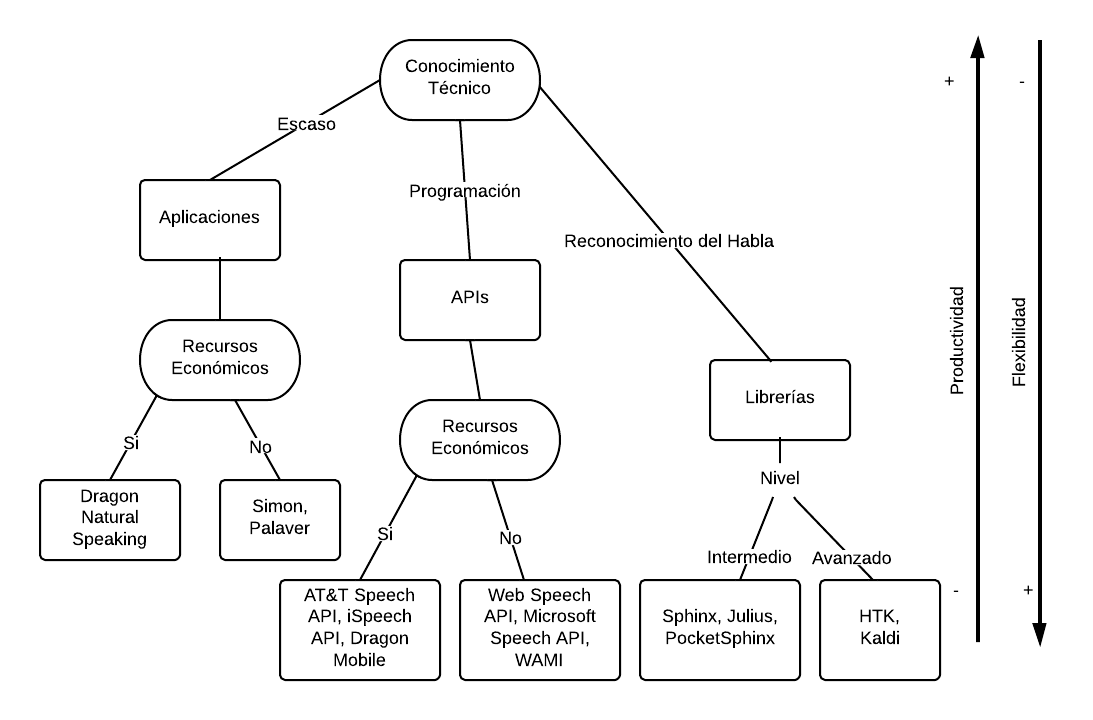
\includegraphics[width=0.9\linewidth]{./graphics/esquema-herramientas.png}
\caption{Esquema representativo de la clasificaci\'on de herramientas para el reconocimiento del habla.}
\label{figure:esquema-herramientas}
\end{figure}

\section{Aplicaciones}
\label{sec:aplicaciones}

% introduccion

Las soluciones de reconocimiento del habla, catalogadas como aplicaciones, propocionan
a los usuarios finales los medios necesarios para realizar determinadas tareas mediante
la voz: dictado autom\'atico, navegaci\'on de interfaces, etc\'etera; sin
la necesidad de tener un conocimiento previo de los conceptos relacionados al
reconocimiento del habla. \'Estas aplicaciones presentan las siguientes 
caracter\'isticas en cuanto a los criterios generales de evaluaci\'on:

\begin{itemize}
    \item Conocimiento t\'ecnico: requieren de poco conocimiento t\'ecnico debido a que \'estas
        soluciones se ofrecen como un producto a los usuarios finales, por lo tanto, sus funcionalidades
        pueden utilizarse directamente sin necesidad de entender los componentes que intervienen
         en el sistema.
    \item Productividad: teniendo en cuenta el criterio anterior, cabe resaltar que con
        las aplicaciones se puede lograr un buen grado de productividad, porque los esfuerzos
        de los usuarios se enfocan en realizar determinadas tareas utilizando las funcionalidades
         disponibles.
    \item Flexibilidad: la flexibilidad para esta categor\'ia de soluciones es reducida, porque las
        funcionalidades que ofrece cada aplicaci\'on se encuentran orientadas a resolver tareas
        espec\'ificas: dictado autom\'atico, para la transcripci\'on de documentos; reconocimiento
        de comandos, para navegar interfaces; reconocimiento del habla, para 
        automatizaci\'on de servicios de operador. Cada aplicaci\'on tiene un \'ambito de aplicabilidad
        lo cual impone un l\'imite en su flexibilidad, en comparaci\'on a otras categor\'ias que
         se ver\'an m\'as adelante.
\end{itemize}

\subsection{Criterios Espec\'ificos de Evaluaci\'on}

Los criterios espec\'ificos nos permiten evaluar a las aplicaciones en cuanto a factores
particulares y relevantes para esta categor\'ia. A continuaci\'on se presentan los criterios 
espec\'ificos de evaluaci\'on para las aplicaciones:

\begin{itemize}
    \item Precio
    \item Soporte para m\'ultiples idiomas
\end{itemize}

\subsection{Ejemplos de Aplicaciones}

\subsubsection{Simon}
\label{sec:simon}

\emph{Simon} es un programa de reconocimiento del habla de c\'odigo abierto que tiene como objetivo
reemplazar el teclado y mouse \cite{SimonListen}. Esta dise\~nado para ser muy flexible y permite la
personalizaci\'on para cualquier aplicaci\'on que necesite incorporar reconocimiento
del habla. Adem\'as, \'este programa pretende ayudar a personas con alguna discapacidad, debido
a que busca brindarles la posibilidad de escribir correos electr\'onicos, navegar internet, etc.

\begin{itemize}
    \item \emph{Precio:} esta herramienta es gratuita y de c\'odigo abierto.
    \item \emph{Soporte para m\'ultiples idiomas:} \emph{Simon} es una herramienta independiente del idioma,
    debido a que permite incorporar nuevos modelos estad\'isticos. Si se desea
	utilizar el espa\~nol, por ejemplo, simplemente hay que incorporar el modelo estad\'istico que representa
    a los sonidos que forman las palabras de dicho idioma.
    \item \emph{Facilidad de configuraci\'on:} esta herramienta est\'a dise\~nada para que sea
	f\'acilmente configurable desde su interfaz gr\'afica. Utiliza el concepto de Escenarios para identificar a un contexto (aplicaci\'on)
	que se desea operar a trav\'es de la voz. Brinda, por defecto, un modelo base para el idioma ingl\'es (el
    modelo prove\'ido por Voxforge\cite{Voxforge}), pero permite incorporar otros modelos e incluso generar nuevos.
    \item \emph{Soporte para dispositivos m\'oviles:} \emph{Simone} es un cliente de Simon para dispositivos m\'oviles. Aunque las
	capacidades de este cliente son limitadas, actualmente permite: controlar una computadora a trav\'es de una red
	local inal\'ambrica (utilizar el tel\'efono como micr\'ofono), realizar llamadas a contactos y navegar el software. 
    La versi\'on inicial de \emph{Simone} se desarroll\'o para 
	Meego\footnote{Meego fue un sistema operativo de c\'odigo abierto que result\'o de la uni\'on de
	los sistemas operativos \emph{Maemo} de Nokia y \emph{Moblin} de Intel, con la intenci\'on de competir
	con el sistema operativo \emph{Android} de Google.}, aunque el soporte para Android se encuentra en desarrollo.

\end{itemize}

\subsubsection{Palaver}
\label{sec:palaver}

\emph{Palaver} es una aplicaci\'on, actualmente disponible solo para Linux orientada principalmente
al control de funcionalidades de las computadoras a trav\'es de la voz, aunque tambi\'en
puede utilizarse para transcripci\'on \cite{Palaver}. \emph{Palaver} utiliza un diccionario para
definir los comandos que soporta y, adem\'as, permite definir nuevos comandos a trav\'es
de un sistema de \foreign{plugins}.

\begin{itemize}
    \item \emph{Precio:} esta herramienta es gratuita y de c\'odigo abierto.
    \item \emph{Soporte para m\'ultiples idiomas:} esta herramienta delega la interpretaci\'on de
	la voz a los servidores de Google, por lo tanto, es posible utilizar \emph{Palaver} en otros idiomas.
    Sin embargo, esto implica la modificaci\'on del diccionario de comandos, ya que por 
    defecto \emph{Palaver} provee un diccionario para el idioma ingl\'es. Adem\'as, al delegar el
    reconocimiento a servidores externos, es necesario tener conexi\'on a internet para utilizar
    esta herramienta.
    \item \emph{Facilidad de configuraci\'on:} esta herramienta permite extender los comandos soportados a 
    trav\'es de un sistema de plugins, adem\'as es posible configurar otros aspectos de la aplicaci\'on
    (como el idioma). 
    Sin embargo, no existe una interfaz gr\'afica para realizar las configuraciones, lo que reduce en
    cierta medida la facilidad de configuraci\'on.
    \item \emph{Soporte para dispositivos m\'oviles:} actualmente esta herramienta no ofrece soporte
    para dispositivos m\'oviles.
\end{itemize}

\subsubsection{Dragon Naturally Speaking}
\label{sec:nuance}

\foreign{Dragon Naturally Speaking} es una aplicaci\'on de la empresa \emph{Nuance Communications} 
que permite interactuar con las computadoras a trav\'es de la voz \cite{DragonNaturallySpeaking}. Permite
crear documentos, escribir correos electr\'onicos, lanzar aplicaciones, abrir archivos, controlar
el mouse, etc. Esta herramienta presenta una interfaz de usuario minimalista y posee tres
\'areas principales de aplicaci\'on: dictado, s\'intesis de habla y reconocimiento de comandos. 
El usuario puede dictar y obtener la transcripci\'on del habla en forma de texto escrito, obtener
una versi\'on sintetizada de un documento como un flujo de audio, y emitir comandos de voz que
son reconocidos por el sistema.

\begin{itemize}
    \item \emph{Precio:} esta herramienta viene en varias ediciones, la \foreign{Home Edition} se puede
        obtener desde \$99.99 y la versi\'on \foreign{Premium} desde \$199.99
    \item \emph{Soporte para m\'ultiples idiomas:} este programa soporta los siguientes idiomas: Ingl\'es, Franc\'es,
	Alem\'an, Espa\~nol, Italiano, Holand\'es. Adem\'as cabe destacar que esta herramienta soporta 
    m\'ultiples acentos.
    \item \emph{Facilidad de configuraci\'on:} esta herramienta presenta una interfaz minimalista a 
    trav\'es de la cual se puede modificar la configuraci\'on del sistema.
    \item \emph{Soporte para dispositivos m\'oviles:} \foreign{Dragon Remote Mic} es una aplicaci\'on para 
    \emph{iOS} y \emph{Android} que permite convertir un tel\'efono celular en un microfono inal\'ambrico 
    para el sistema. Adem\'as, la empresa \foreign{Nuance Communications} proporciona otros productos, 
    derivados de \foreign{Dragon}, orientados a dispositivos m\'oviles.
\end{itemize}


%!TEX root = ../../tesis.tex
\section{Interfaces de Programaci\'on de Aplicaciones}
\label{apis}

% introduccion

Una interfaz de programaci\'on de aplicaciones (tambi\'en conocida como \gls{api} por sus siglas 
en ingl\'es) proporciona a los desarrolladores los medios necesarios para integrar funcionalidades de
reconocimiento del habla al \foreign{software} que implementan, sin necesidad de poseer
conocimiento en detalle del \'area. De acuerdo a los criterios de evaluaci\'on generales, 
pueden mencionarse las siguientes caracter{\'\i}sticas:

\begin{itemize}
 	\item Conocimiento t\'ecnico necesario: aunque no requieren conocimiento sobre detalles de implementaci\'on
 	del \'area de reconocimiento del habla, si resultan necesarios conocimientos b\'asicos de
 	programaci\'on, por lo cual resulta inadecuada su utilizaci\'on por parte de usuarios finales.
 	\item Productividad: la utilizaci\'on de una interfaz de programaci\'on de aplicaciones permite
 	al desarrollador abstraerse de la complejidad subyacente del problema, lo cual resulta en
 	un alto grado de productividad. Sin embargo, el ocultamiento de los detalles del proceso
 	puede ser un factor negativo en algunos \'ambitos, como el \mbox{acad\'emico}.
 	\item Flexibilidad: estas herramientas presentan un buen grado de flexibilidad, debido a
 	que no est\'an orientadas a una tarea en particular. La selecci\'on del problema espec{\'\i}fico
 	que se soluciona utilizando reconocimiento del habla es responsabilidad del desarrollador
 	que utiliza la interfaz. Cabe destacar, sin embargo, que los componentes propios de la
 	implementaci\'on de la interfaz de programaci\'on, al estar ocultos, no
 	pueden modificarse.
 \end{itemize}


\subsection{Criterios Espec\'ificos de Evaluaci\'on}

Los criterios espec{\'\i}ficos seg\'un los cuales se evaluar\'an las opciones disponibles en esta
categor{\'\i}a son:

\begin{itemize}
	\item Empresa o Instituci\'on Responsable
	\item Precio o Inversi\'on econ\'omica
	\item Soporte para m\'ultiples idiomas
	\item Soporte Offline
	\item Dependencia de Plataforma
\end{itemize}


\subsection{Ejemplos de Interfaces de Programaci\'on de Aplicaciones}

%!TEX root = ../../tesis.tex
\subsubsection{Web Speech API}
\label{sec:webspeech}

La \foreign{Web Speech API} define un est\'andar que especifica una interfaz de programaci\'on de aplicaciones para permitir
a los desarrolladores web incorporar s{\'\i}ntesis y reconocimiento del habla a sus sitios web.

\begin{itemize}
	\item \emph{Empresa o Instituci\'on Responsable:} La especificaci\'on de la interfaz fue
	publicada por el \foreign{Speech API Community Group} del
	\mbox{\foreign{World Wide Web Consortium} \cite{GoogleWebSpeechAPI}.}
	La \'unica implementaci\'on disponible fue desarrollada por \foreign{Google} para su navegador \foreign{Chrome}.
	\item \emph{Precio:} la utilizaci\'on de esta herramienta a trav\'es de \foreign{Google Chrome} es gratuita e
	ilimitada en la actualidad. Aunque esto podr\'ia llegar a cambiar ya que se trata del producto de una empresa
    en particular.
	\item \emph{Soporte para m\'ultiples idiomas:} la interfaz ofrece soporte para m\'as de 30 idiomas.
	\item \emph{Soporte Offline:} la especificaci\'on publicada de la interfaz no limita ni reglamenta su
	implementaci\'on; sin embargo, la \'unica opci\'on funcional actualmente delega el procesamiento a los
	servidores de \foreign{Google}, por lo cual requiere de una conexi\'on a internet para su uso.
	\item \emph{Dependencia de Plataforma:} es necesario un navegador web para su utilización.
	Aunque actualmente solo puede utilizarse a trav\'es de \foreign{Chrome}, implementar la interfaz
	para otros navegadores es posible. No existe dependencia con el sistema operativo.
\end{itemize}


%!TEX root = ../../tesis.tex
\subsubsection{\gls{att} Speech \gls{api}}
\label{sec:att}

La \foreign{\gls{att} Speech \gls{api}} \cite{AttSpeech} define una interfaz de programaci\'on de aplicaciones para permitir
a los desarrolladores incorporar s{\'\i}ntesis y reconocimiento del habla en aplicaciones m\'oviles,
web o de escritorio. El procesamiento se lleva a cabo a trav\'es del motor \foreign{\gls{att} Watson}.

\begin{itemize}
	\item \emph{Empresa o Instituci\'on Responsable:} \foreign{\gls{att} Inc}.
	\item \emph{Precio:} un mill\'on de llamadas a la interfaz por 99\$ anuales, llamadas adicionales a un centavo
	cada una.
	\item \emph{Soporte para m\'ultiples idiomas:} el ingl\'es es el principal idioma soportado, aunque incluye
	soporte reducido para el espa\~nol.
	\item \emph{Soporte Offline:} al delegarse el procesamiento a los servidores de \foreign{\gls{att}},
	una conexi\'on a internet es indispensable para su uso.
	\item \emph{Dependencia de Plataforma:} al ofrecer una interfaz \gls{rest}, no existe dependencia con navegador
	ni con sistema operativo alguno. Adem\'as, se ofrecen varios \gls{sdk}s para facilitar
	el desarrollo en plataformas como \foreign{Windows}, \foreign{iOS} y \foreign{Android}.
\end{itemize}

%!TEX root = ../../tesis.tex
\subsubsection{Microsoft Speech \gls{api}}
\label{sec:microsoft}

La \foreign{Microsoft Speech \gls{api}} es una interfaz de programaci\'on de aplicaciones orientada a
facilitar la integraci\'on de s{\'\i}ntesis y reconocimiento del habla con el sistema operativo \foreign{Windows}
y las aplicaciones que se ejecutan sobre el mismo \cite{MicrosoftSpeech}. Aplicaciones como \foreign{Microsoft Office}
utilizan esta interfaz para ofrecer modelos de interacci\'on multimodal\footnote{Las interfaces multimodales
ofrecen al usuario final distintas formas de interactuar con el sistema.}con el usuario.

\begin{itemize}
	\item \emph{Empresa o Instituci\'on Responsable:} \foreign{Microsoft}.
	\item \emph{Precio:} esta herramienta est\'a incluida en el sistema operativo \foreign{Windows}, aunque
	tambi\'en puede descargarse por separado de manera gratuita.
	\item \emph{Soporte para m\'ultiples idiomas:} esta herramienta ofrece soporte para 26 idiomas,
	entre los cuales se encuentra el espa\~nol.
	\item \emph{Soporte Offline:} esta herramienta se encuentra integrada con el sistema operativo
	y realiza el procesamiento de manera local, por lo cual puede utilizarse sin conexi\'on a internet.
	\item \emph{Dependencia de Plataforma:} esta interfaz es estrictamente dependiende del sistema operativo,
	siendo utilizable solo con \foreign{Microsoft Windows}.
\end{itemize}

%!TEX root = ../../tesis.tex
\subsubsection{WAMI}
\label{sec:wami}

WAMI es un \foreign{toolkit} desarrollado en el Instituto Tecnol\'ogico de
\mbox{Massachusetts \cite{WamiHome}}. T\'ecnicamente, es m\'as que una interfaz de programaci\'on
de aplicaciones; ofrece un conjunto de herramientas, para el lado servidor y el lado cliente,
que permiten al desarrollador ofrecer su propia implementaci\'on de la interfaz.

WAMI est\'a orientado a ofrecer una interfaz web para un determinado reconocedor del habla,
como Sphinx, Julius, u otro. A\'un as{\'\i}, el MIT ofrece un reconocedor del habla que implementa
la interfaz para fines de prototipado como parte del proyecto.

\begin{itemize}
	\item \emph{Empresa o Instituci\'on Responsable:} Instituto Tecnol\'ogico de Massachusetts.
	\item \emph{Precio:} esta herramienta es gratuita y de c\'odigo abierto.
	\item \emph{Soporte para m\'ultiples idiomas:} la implementaci\'on para prototipado ofrecida
	por el MIT soporta los idiomas ingl\'es, chino y japon\'es. El soporte para idiomas de WAMI
	depende exclusivamente del reconocedor con cual se integre.
	\item \emph{Soporte Offline:} WAMI se basa en la arquitectura cliente--servidor, por lo cual
	es necesaria una conexi\'on entre ambos.
	\item \emph{Dependencia de Plataforma:} al ofrecer una interfaz REST, no existe dependencia con
	navegador ni con sistema operativo alguno.
\end{itemize}

%!TEX root = ../../tesis.tex
\subsubsection{iSpeech \gls{api}}
\label{sec:ispeech}

La \foreign{iSpeech \gls{api}} \cite{iSpeech} define una interfaz de programaci\'on de aplicaciones para permitir
a los desarrolladores incorporar s{\'\i}ntesis y reconocimiento del habla en aplicaciones m\'oviles,
web o de escritorio.

\begin{itemize}
	\item \emph{Empresa o Instituci\'on Responsable:} \foreign{iSpeech}, una empresa estadounidense dedicada a
	proveer reconocimiento y s{\'\i}ntesis del habla como servicio. Su producto m\'as reconocido es la aplicaci\'on m\'ovil
	\foreign{Drivesafe.ly}, orientada a reducir las distracciones de un conductor.
	\item \emph{Precio:} Gratis para aplicaciones m\'oviles sin fines comerciales. De 0,02\$ a 0,0001\$ por
	transacci\'on, dependiendo del tama\~no de la compra, para otros usos.
	\item \emph{Soporte para m\'ultiples idiomas:} soporta reconocimiento cont{\'\i}nuo (sin pausas) del habla para 6 idiomas,
	entre ellos el espa\~nol, y reconocimiento de vocabulario reducido para m\'as de 10 idiomas.
	\item \emph{Soporte Offline:} el procesamiento se realiza en los servidores de \foreign{iSpeech}, por lo cual
	una conexi\'on a internet es indispensable para su uso.
	\item \emph{Dependencia de Plataforma:} al ofrecer una interfaz \gls{rest}, no existe dependencia con navegador
	ni con sistema operativo alguno. Adem\'as, se ofrecen varios \gls{sdk} para facilitar
	el desarrollo en m\'ultiples plataformas y lenguajes de programaci\'on.
\end{itemize}
%!TEX root = ../../tesis.tex
\subsubsection{Dragon Mobile}
\label{sec:dragonmobile}

\foreign{Dragon Mobile} ofrece una interfaz de programaci\'on de aplicaciones para permitir
a los desarrolladores incorporar s{\'\i}ntesis y reconocimiento del habla a sus
\mbox{aplicaciones \cite{DragonMobile}}. Est\'a espec{\'\i}ficamente orientado al desarrollo de
aplicaciones para plataformas m\'oviles.

\begin{itemize}
	\item \emph{Empresa o Instituci\'on Responsable:} \foreign{Nuance Communications}.
	\item \emph{Precio:} el uso de esta herramienta es gratuito para aplicaciones sin fines comerciales.
	Desde 0.08\$ a 0.006\$ por transacci\'on, dependiendo del tama\~no de la compra, para otros usos.
	Para comercializar una aplicaci\'on que utiliza esta herramienta, es necesaria una inversi\'on inicial
	m{\'\i}nima de 3000\$.
	\item \emph{Soporte para m\'ultiples idiomas:} se ofrece soporte para m\'as de 20 idiomas, entre ellos
	el espa\~nol.
	\item \emph{Soporte Offline:} al delegarse el procesamiento a los servidores de \foreign{Nuance},
	una conexi\'on a internet es indispensable para su uso.
	\item \emph{Dependencia de Plataforma:} al ofrecer una interfaz \gls{rest}, no existe dependencia con navegador
	ni con sistema operativo alguno. Adem\'as, se ofrecen varios \gls{sdk} para facilitar
	el desarrollo en plataformas m\'oviles como \foreign{Windows Phone}, \foreign{iOS} y \foreign{Android}.
\end{itemize}

\section{Librer\'ias y Frameworks}
\label{sec:librerias}

Una librer{\'\i}a va m\'as all\'a de una especificaci\'on de interacci\'on y el c\'odigo fuente que permita cumplirla.
Una librer{\'\i}a incluye un conjunto de funcionalidades o m\'etodos cuyo modo de utilizaci\'on queda a criterio
del desarrollador. En el caso de un framework, se incluyen tambi\'en ciertos patrones de dise\~no para la aplicaci\'on.

Aunque la distinci\'on entre una librer{\'\i}a y una interfaz de programaci\'on de aplicaciones puede resultar
sutil, para este trabajo, se consideran el mayor grado de control y el menor nivel de abstracci\'on
como criterios para identificar una herramienta como una librer{\'\i}a.

As{\'\i}, una interfaz de programaci\'on de aplicaciones es una especificaci\'on de interacci\'on con un componente
reconocedor del habla completamente implementado, mientras que una librer{\'\i}a puede verse como un conjunto
de bloques que permiten al desarrollador construir su propio reconocedor del habla a medida.

De acuerdo a los criterios de evaluaci\'on generales, las siguientes caracter{\'\i}sticas pueden mencionarse:

\begin{itemize}
 	\item Conocimiento t\'ecnico necesario: la utilizaci\'on de librer{\'\i}as requiere conocimiento t\'ecnico
 	espec{\'\i}fico del \'area del reconocimiento del habla por parte del programador, debido a que el nivel de
 	abstracci\'on es menor al de las herramientas previamente descriptas.
 	\item Productividad: Debido al alto grado de control que ofrecen, el desarrollo de los distintos
 	elementos de un sistema de reconocimiento del habla requiere de m\'as trabajo de an\'alisis e implementaci\'on.
 	Esto resulta en una productividad baja en comparaci\'on con otras alternativas, que permiten al
 	programador abstraerse de los detalles del proceso de reconocimiento del habla.
 	A\'un as{\'\i} en ciertos \'ambitos, como el acad\'emico, la posibilidad de conocer y manipular los distintos
 	componentes del mencionado proceso representa una importante ventaja que ofrecen estas herramientas.
 	\item Flexibilidad: las librer{\'\i}as ofrecen un alto grado de flexibilidad, siendo la alternativa
 	m\'as adaptable de entre las categor{\'\i}as analizadas. Componentes importantes de un sistema
 	de reconocimiento del habla como el modelo de lenguaje, el modelo ac\'ustico y los algoritmos involucrados
 	pueden seleccionarse, modificarse o incluso reimplementarse de acuerdo al criterio del desarrollador.
 \end{itemize}

\subsection{Criterios Espec\'ificos de Evaluaci\'on}

Los criterios espec{\'\i}ficos seg\'un los cuales se evaluar\'an las opciones disponibles en esta
categor{\'\i}a son:

\begin{itemize}
	\item Empresa o Instituci\'on Responsable
	\item Precio
	\item Licencia
	\item Soporte para m\'ultiples idiomas
	\item Dependencia de Plataforma
	\item Modelos de Lenguaje Aceptados
	\item Modelos Ac\'usticos Aceptados
	\item Uso de Memoria
\end{itemize}


\subsection{Ejemplos de librer{\'\i}as o frameworks}

%!TEX root = ../../tesis.tex
\subsubsection{Sphinx 4}
\label{sec:sphinx}

La librer{\'\i}a Sphinx 4 es un sistema de reconocimiento del habla de c\'odigo abierto desarrollado en
la Universidad \mbox{\foreign{Carnegie Mellon} \cite{Sphinx4}}. La misma est\'a implementada
completamente en el lenguaje de programaci\'on Java, y permite la utilizaci\'on de modelos de lenguaje,
modelos ac\'usticos y diccionarios fon\'eticos construidos por el propio desarrollador utilizando las
herramientas proveídas por la librer\'ia.

Esta herramienta est\'a orientada principalmente a la escalabilidad y a la integraci\'on con
componente externos, facilitando la implementaci\'on, por ejemplo, de sistema de reconocimiento del
habla en la nube.

\begin{itemize}
	\item \emph{Empresa o Instituci\'on Responsable:} Universidad \foreign{Carnegie Mellon}.
	\item \emph{Precio:} esta herramienta puede utilizarse de forma gratuita.
	\item \emph{Licencia:} Sphinx 4 se distribuye bajo una licencia basada en la \gls{bsd}, considerada
	de c\'odigo abierto. Un \'unico componente, la \foreign{Java Speech \gls{api}} debe descargarse por
	separado por no ser de c\'odigo abierto, aunque puede obtenerse de manera gratuita.
	\item \emph{Soporte para m\'ultiples idiomas:} existen modelos ac\'usticos construidos para
	8 idiomas, entre ellos el espa\~nol, aunque la calidad de los mismos var{\'\i}a.
	De todas formas, el desarrollador puede construir sus propios modelos con las herramientas
	que provee la librer{\'\i}a, con lo cual puede brindarse soporte para otros idiomas.
	\item \emph{Dependencia de Plataforma:} puede utilizarse cualquier plataforma para la cual
	exista una versi\'on de la m\'aquina virtual de Java disponible.
	\item \emph{Modelos de Lenguaje Aceptados:} se aceptan modelos de lenguaje basados en una
        gram\'atica, en formato JGSF (\foreign{Java Speech Grammar Format}), y modelos de 
        lenguaje estad{\'\i}sticos, basados en bigramas y trigramas en formato \gls{arpa} (\foreign{Advanced Research Projects Agency}).
	\item \emph{Modelos Ac\'usticos Aceptados:} Sphinx define su propio formato de modelos ac\'usticos,
	en el cual existen modelos ya construidos para 8 idiomas. Adem\'as, se ofrecen las herramientas
	necesarias para construir un modelo ac\'ustico propio.
	\item \emph{Uso de Memoria:} esta herramienta no se recomienda para sistemas con poca memoria,
	debido a que depende de la m\'aquina virtual de Java para ejecutarse.
\end{itemize}

%!TEX root = ../../tesis.tex
\subsubsection{PocketSphinx}
\label{sec:pocketsphinx}

La librer{\'\i}a Pocketsphinx es desarrollada en paralelo a Sphinx 4 en la Universidad
\mbox{\foreign{Carnegie Mellon} \cite{PocketSphinxHomePage}}. Esta herramienta de c\'odigo abierto
est\'a implementada en el lenguaje C, logr\'andose con esto en un mayor rendimiento y facilidad
para desarrollar \foreign{bindings} para otros lenguajes de programaci\'on.

Pocketsphinx est\'a orientado a la optimizaci\'on del rendimiento y a la portabilidad a distintas
plataformas, resultando particularmente adecuada para la implementaci\'on de sistemas empotrados
y sistemas en tiempo \mbox{real \cite{HugginsDainesPocketSphinx2006}}.

\begin{itemize}
	\item \emph{Empresa o Instituci\'on Responsable:} Universidad \foreign{Carnegie Mellon}.
	\item \emph{Precio:} esta librer\'ia puede utilizarse de forma gratuita.
	\item \emph{Licencia:} Pocketsphinx  se distribuye bajo una versi\'on simplificada de la licencia
	\gls{bsd}, considerada de c\'odigo abierto.
	\item \emph{Soporte para m\'ultiples idiomas:} Pocketsphinx utiliza los mismos modelos
	que \mbox{Sphinx 4}, por lo que el soporte para idiomas es similar. Se ofrece soporte para 8
	idiomas, aunque puede extenderse a otros mediante las herramientas prove{\'\i}das.
	\item \emph{Dependencia de Plataforma :} esta librer\'ia puede utilizarse en sistemas operativos
	basados en Unix y en Windows. Adem\'as, cabe destacar la documentaci\'on existente para su instalaci\'on
	en plataformas m\'oviles como Android, iOS y el Kindle de Amazon.
	\item \emph{Modelos de Lenguaje Aceptados:} se utilizan los mismos modelos de lenguaje que \mbox{Sphinx 4},
	basados en gram\'aticas en formato JGSF y modelos estad{\'\i}sticos en formato \gls{arpa}.
	\item \emph{Modelos Ac\'usticos Aceptados:} tambi\'en los modelos ac\'usticos se comparten con \mbox{Sphinx 4}.
	Existen modelos para 8 idiomas ya construidos, y pueden construirse modelos adicionales.
	\item \emph{Uso de Memoria:} el consumo de memoria de Pocketsphinx es muy reducido en comparaci\'on con
        Sphinx 4\cite{SphinxVersions}.
\end{itemize}
%!TEX root = ../../tesis.tex
\subsubsection{HTK}
\label{sec:htk}

\gls{htk}, es un conjunto de herramientas
desarrolladas por el Departamento de Ingenier{\'\i}a de la Universidad de Cambridge. Est\'a constituido
por varias librer{\'\i}as y herramientas ejecutables implementadas en el \mbox{lenguaje C \cite{HTKHomePage}}.

Esta herramienta ofrece un alto grado de personalizaci\'on, por lo que se requiere un nivel considerable
de conocimiento t\'ecnico para implementar un sistema de reconocimiento del habla con la misma.
Cabe destacar que la \'ultima versi\'on estable de \gls{htk} fue lanzada en el a\~no 2009.

\begin{itemize}
	\item \emph{Empresa o Instituci\'on Responsable:} Universidad de Cambridge.
	\item \emph{Precio:} esta herramienta puede utilizarse de forma gratuita.
	\item \emph{Licencia:} aunque el c\'odigo fuente de \gls{htk} puede obtenerse y modificarse,
	la redistribuci\'on del mismo est\'a prohibida. Los modelos generados con \gls{htk} pueden
	redistribuirse libremente.
	\item \emph{Soporte para m\'ultiples idiomas:} \gls{htk} no provee soporte para ning\'un
	idioma directamente, pero proporciona herramientas para la definici\'on de los modelos necesarios.
	\item \emph{Dependencia de Plataforma:} esta herramienta puede utilizarse en sistemas operativos
	basados en Unix y en Windows.
	\item \emph{Modelos de Lenguaje Aceptados:} se utilizan los mismos modelos de lenguaje que \mbox{Sphinx 4},
	basados en gram\'aticas y modelos estad{\'\i}sticos en formato \gls{arpa}.
	\item \emph{Modelos Ac\'usticos Aceptados:} \gls{htk} define su propio formato de modelos ac\'usticos.
	\item \emph{Uso de Memoria:} la documentaci\'on de \gls{htk} hace \'enfasis en que el consumo de memoria depende en
	gran medida de la aplicaci\'on, mencionando 150 MB para la construcci\'on de modelos para un sistema de
	dictado como un ejemplo de niveles altos de utilizaci\'on de este recurso.
	Esta cantidad de memoria no resulta muy elevada para el \foreign{hardware} de una m\'aquina promedio actual.
\end{itemize}
\subsection{Julius}
\label{sec:julius}

%!TEX root = ../../tesis.tex
\subsubsection{Kaldi}
\label{sec:kaldi}

Kaldi es un \foreign{toolkit} de reconocimiento del habla que comenz\'o a desarrollarse durante un taller
en la Universidad \foreign{John Hopkins} en el a\~no 2009. Su desarrollo continu\'o con el apoyo del gobierno
de Rep\'ublica Checa en la \mbox{Universidad de Brno \cite{Povey_ASRU2011}}.

Kaldi est\'a constituida por un conjunto de librer{\'\i}as C++ y herramientas ejecutables. Por su orientaci\'on y
alcance es comparable al proyecto \gls{htk}, resultando tambi\'en necesario un alto nivel de conocimiento t\'ecnico
para su utilizaci\'on.

Cabe destacar su integraci\'on con \gls{fst} para la
construcci\'on de modelos de lenguaje, la cual lo distingue de las dem\'as herramientas analizadas en esta secci\'on.

\begin{itemize}
	\item \emph{Empresa o Instituci\'on Responsable:} Agencia Tecnol\'ogica de Rep\'ublica Checa.
	\item \emph{Precio:} esta herramienta puede utilizarse de forma gratuita.
	\item \emph{Licencia:} Kaldi se distribuye bajo la licencia Apache 2.0, considerada de c\'odigo 
	abierto.
	\item \emph{Soporte para m\'ultiples idiomas:} Kaldi no provee soporte para ning\'un
	idioma directamente, pero proporciona herramientas para la definici\'on de los modelos 
	\mbox{necesarios.}
	\item \emph{Dependencia de Plataforma:} esta herramienta puede utilizarse en sistemas operativos
	basados en \foreign{Unix} y en \foreign{Windows}.
	\item \emph{Modelos de Lenguaje Aceptados:} se proveen herramientas para convertir modelos en formato
	\gls{arpa} a \gls{fst}s.
	\item \emph{Modelos Ac\'usticos Aceptados:} Kaldi define su propio formato de modelos ac\'usticos.
	\item \emph{Uso de Memoria:} no se encontraron datos espec{\'\i}ficos respecto al consumo de memoria
	de Kaldi.
\end{itemize}


\section{Resumen}

A modo de resumen del contenido expuesto en este cap\'itulo, \'esta secci\'on presentar\'a tablas que describen los criterios generales y espec\'ificos
para cada categor\'ia. A continuaci\'on en la tabla~\ref{sec:resumen-herramientas} se pueden observar las distintas
herramientas presentadas.

\begin{table}[H]
\centering
\footnotesize
\begin{tabular}{|p{3.5cm}|>{\centering}p{3.5cm}|>{\centering}p{3.5cm}|>{\centering}p{3.5cm}|}
\hline
                               & Aplicaciones             &  \gls{api}s                            & Librer\'ias/\foreign{Frameworks} \tabularnewline
\hline
Conocimiento T\'ecnico         &     Bajo                    & Medio                            & Alto    \tabularnewline \hline
Productividad                  &     Alto                    & Medio                            & Bajo    \tabularnewline \hline
Flexibilidad                   &     Bajo                    & Medio                            & Alto    \tabularnewline \hline
Alternativas  Propietarias      & \begin{itemize} \setlength{\itemsep}{1pt} \setlength{\parskip}{0pt} \setlength{\parsep}{0pt}\item Dragon Natural Speaking \end{itemize}  & \begin{itemize}  \setlength{\itemsep}{1pt} \setlength{\parskip}{0pt} \setlength{\parsep}{0pt} \item Web Speech \gls{api} \item \gls{att} Speech \gls{api} \item Microsoft Speech \gls{api} \item iSpeech \gls{api} \item Dragon Mobile \end{itemize}  &  \tabularnewline \hline
Alternativas de C\'odigo abierto & \begin{itemize}  \setlength{\itemsep}{1pt} \setlength{\parskip}{0pt} \setlength{\parsep}{0pt} \item Simon \item Palaver \end{itemize}          &           & \begin{itemize} \setlength{\itemsep}{1pt} \setlength{\parskip}{0pt} \setlength{\parsep}{0pt} \item Sphinx 4 \item PocketSphinx \item \gls{htk} \item Julius \item Kaldi \end{itemize} \tabularnewline
\hline
\end{tabular}
\caption{Resumen general de las herramientas}
\label{sec:resumen-herramientas}
\end{table}

\subsection{Aplicaciones}

A continuaci\'on se puede observar una comparaci\'on entre las aplicaciones presentadas respecto a los criterios espec\'ificos
para \'esta categor\'ia


\begin{table}[H]
\centering
\footnotesize
\begin{tabular}{|p{3.5cm}|p{3.5cm}|p{3.5cm}|p{3.5cm}|}
\hline
                                      &  Simon                                                       &  Palaver                                       & Dragon Naturally Speaking \\
\hline
Precio                                & Gratuito                                                     & Gratuito                                       & Desde 99\$  \\ \hline
Soporte para m\'ultiples idiomas      & Si                                                           & Si                                             & Si \\ \hline
Facilidad de configuraci\'on          & F\'acil                                    & Reducida                                       & F\'acil \\ \hline
Soporte para dispositivos m\'oviles   & Si                                                           & No                                             & Si, mediante otros productos \\
\hline
\end{tabular}
\caption{Resumen de los criterios espec\'ificos de las aplicaciones}
\label{sec:resumen-aplicaciones}
\end{table}

\subsection{Interfaz de Programaci\'on de Aplicaciones}

En las tablas~\ref{sec:resumen-apis} y~\ref{sec:resumen-apis-2} se puede observar una comparaci\'on entre las \gls{api}s presentadas, respecto a los criterios espec\'ificos
para \'esta categor\'ia


\begin{table}[H]
\centering
\footnotesize
\begin{tabular}{|p{3.5cm}|p{3.5cm}|p{3.5cm}|p{3.5cm}|}
\hline
                                      &  Web Speech \gls{api} & \gls{att} Speech \gls{api} & Microsoft Speech \gls{api} \\
\hline
Empresa o Instituci\'on responsable & \foreign{Speech API Community Group}. Implementado actualmente por \foreign{Google}  &  \gls{att} Inc.  & Microsoft\\ \hline
Precio                              & Gratuito, a trav\'es de Google Chrome  & Un mill\'on de llamadas a la \gls{api} por 99\$ anuales. 0.01\$ por llamada extra  & Gratuito\\ \hline
Soporte para m\'ultiples idiomas    & Si  & 2 idiomas & Si\\ \hline
Soporte Offline                     & No  & No  & Si \\ \hline
Dependencia de Plataforma           & No  & No & Si, solo para \emph{Microsoft Windows} \\
\hline
\end{tabular}
\caption{Resumen de los criterios espec\'ificos de las APIs. Primera parte.}
\label{sec:resumen-apis}
\end{table}


\begin{table}[H]
\centering
\footnotesize
\begin{tabular}{|p{3.5cm}|p{3.5cm}|p{3.5cm}|p{3.5cm}|}
\hline
                                      &  \gls{wami} & iSpeech \gls{api} & Dragon Mobile \\
\hline
Empresa o Instituci\'on responsable & Instituto Tecnol\'ogico de Massachusetts & \foreign{iSpeech}  & \foreign{Nuance Communications} \\ \hline
Precio &  Gratuito  & Gratuito para aplicaciones no comerciales. De 0.02\$ a 0.0001\$ para otros usos & Gratuito para aplicaciones no comerciales. De 0.08\$ a 0.006\$ para otros usos. \\ \hline
Soporte para m\'ultiples idiomas  & No, aunque depende del reconocedor utilizado & Si & Si \\ \hline
Soporte Offline & No & No & No\\ \hline
Dependencia de Plataforma & No & No & No\\
\hline
\end{tabular}
\caption{Resumen de los criterios espec\'ificos de las APIs. Segunda parte.}
\label{sec:resumen-apis-2}
\end{table}


\subsection{Librer\'ias/\emph{Frameworks}}

A continuaci\'on, las tablas~\ref{sec:resumen-libs} y~\ref{sec:resumen-libs-2} muestran una comparaci\'on entre las librer\'ias presentadas, respecto a los criterios espec\'ificos
para \'esta categor\'ia


\begin{table}[H]
\centering
\footnotesize
\begin{tabular}{|p{3.5cm}|p{3.5cm}|p{3.5cm}|p{3.5cm}|}
\hline
                                  &  Sphinx 4 & PocketSphinx & \gls{htk} \\
\hline
Empresa o Instituci\'on Responsable & Universidad \foreign{Carnegie Mellon} & Universidad \foreign{Carnegie Mellon} & Universidad de Cambridge \\ \hline
Precio & Gratuito & Gratuito & Gratuito \\ \hline
Licencia & \gls{bsd}, con un componente privativo & \gls{bsd} simplificada & C\'odigo fuente modificable, se prohibe su redistribuci\'on.\\ \hline
Soporte para m\'ultiples idiomas & Si & Si & No\\ \hline
Dependencia de Plataforma & No & No & No \\ \hline
Modelos de Lenguaje Aceptados & JGSF, bigramas y trigamas &  JGSF, bigramas y trigamas &  JGSF, bigramas y trigamas \\ \hline
Modelos Ac\'usticos Aceptados & Modelo propio & Modelo propio &  Modelo propio \\ \hline
Uso de Memoria & No se recomienda para sistemas de poca memoria & Reducido en comparaci\'on a Sphinx 4 & Dependiente de la aplicaci\'on \\
\hline
\end{tabular}
\caption[Resumen de los criterios espec\'ificos de las Librer\'ias/\foreign{Frameworks}.\protect\newline Primera parte.]
{Resumen de los criterios espec\'ificos de las Librer\'ias/\foreign{Frameworks}. Primera parte.}
\label{sec:resumen-libs}
\end{table}

\begin{table}[H] 
\centering
\footnotesize
\begin{tabular}{|p{3.5cm}|p{3.5cm}|p{3.5cm}|}
\hline
                                  &  Julius & Kaldi \\
\hline
Empresa o Instituci\'on Responsable &  \foreign{Interactive Speech Technology Consortium} & Agencia Tecnol\'ogica de Rep\'ublica Checa \\ \hline
Precio & Gratuito & Gratuito \\ \hline
Licencia & \gls{bsd} & Apache 2.0 \\ \hline
Soporte para m\'ultiples idiomas & No &  No \\ \hline
Dependencia de Plataforma & No & No \\ \hline
Modelos de Lenguaje Aceptados & Basados en gram\'aticas y modelos en formato \gls{arpa} & Modelos en formato \gls{fst} \\ \hline
Modelos Ac\'usticos Aceptados & Modelo propio & Modelo propio \\ \hline
Uso de Memoria & Bajo & \\
\hline
\end{tabular}
\caption[Resumen de los criterios espec\'ificos de las librer\'ias/\foreign{framework}s.\protect\newline Segunda parte.]{Resumen de los criterios espec\'ificos de las librer\'ias/\foreign{framework}s. Segunda parte.}
\label{sec:resumen-libs-2}
\end{table}

%!TEX root = ../tesis.tex
\chapter{Definici\'on del Problema}
\label{sec:problema}

% introduccion

%!TEX root = ../tesis.tex
\section{Descripci\'on General}
\label{sec:problema-general}

El reconocimiento del habla (tambi\'en conocido como reconocimiento autom\'atico del habla) es el proceso
de convertir una se\~nal de voz en una secuencia de palabras, mediante un algoritmo implementado
como programa \mbox{computacional \cite{JaisalAReview2012}}.

Las interfaces mediante voz del usuario son sistemas computaciones especializados que permiten la
interacci\'on entre seres humanos y computadoras (otros sistemas computacionales) a trav\'es de
s{\'\i}ntesis y reconocimiento del habla. Estas interfaces presentan ciertas caracter{\'\i}sticas que las
distinguen de las interfaces visuales \cite{GabrielVoice2007}:

\begin{itemize}
	\item Transitoriedad: la voz desaparece tan pronto como se termina de pronunciar una oraci\'on,
	lo cual obliga a recordar lo que se dijo. Las interfaces visuales, por otro lado, son persistentes.
	\item Invisibilidad: la voz no es visible, lo cual hace dif{\'\i}cil indicar al usuario las opciones
	disponibles y los comandos necesarios para ejecutarlas. En las interfaces visuales los men\'ues
	cumplen esta funci\'on.
	\item Asimetr{\'\i}a: la voz puede producirse r\'apidamente, pero comprender lo que se escucha requiere
	m\'as tiempo. As{\'\i}, un usuario puede hablar m\'as r\'apido de lo que escribe con un teclado; sin embargo,
	al usuario le toma m\'as tiempo comprender lo que escucha que lo que lee.
\end{itemize}

Estas caracter{\'\i}sticas suponen un desaf{\'\i}o adicional al momento de dise\~nar interfaces mediante voz del
usuario. A\'un as{\'\i}, estas interfaces poseen un gran potencial en situaciones en las cuales la
combinaci\'on tradicional de teclado, rat\'on y monitor resulta problem\'atica \cite{NielsenVoice2003}:

\begin{itemize}
	\item Usuarios con discapacidades, las cuales les impiden manejar apropiadamente el rat\'on y/o
	el teclado o visualizar la informaci\'on en el monitor.
	\item Usuarios en situaciones de manos y vista ocupadas: como la conducci\'on de un veh{\'\i}culo o
	la reparaci\'on de equipamiento complejo.
	\item Usuarios sin acceso a un teclado o monitor: en este caso los usuarios podr{\'\i}an acceder
	a un sistema a trav\'es de un tel\'efono convencional.
\end{itemize}


%!TEX root = ../tesis.tex
\section{Alcance}
\label{sec:problema-especifico}

De modo a contrastar la pr\'actica con el conocimiento te\'orico adquirido en
el transcurso de este trabajo de investigaci\'on, se incluye el dise\~no e implementaci\'on de
una interfaz mediante voz del usuario para una aplicaci\'on como parte del mismo.

Para obtener conclusiones del proceso de dise\~no e implementaci\'on y de la posterior evaluaci\'on
de la interfaz, se consider\'o que la misma deb{\'\i}a ser de cierta complejidad. Esto es, la
aplicaci\'on implementada deb{\'\i}a cumplir con los siguientes requisitos:

\begin{itemize}
     \item Nivel de interacci\'on medio o alto entre el usuario y la aplicaci\'on.
     \item Lenguaje de tama\~no considerable.
     \item Comandos reconocidos de varias longitudes.
     \item Interacci\'on normalmente prolongada entre el usuario y la aplicaci\'on.
 \end{itemize} 

Cumpliendo con las condiciones anteriormente mencionadas, se decidi\'o dise\~nar e implementar 
una interfaz para un programa simple de composici\'on musical.
Se opt\'o por utilizar una interfaz multimodal, 
haciendo uso de soporte visual para minimizar el efecto de las limitaciones
relacionadas a la voz que se mencionaron previamente.

Las funcionalidades m{\'\i}nimas requeridas para el sistema se citan a continuaci\'on:
%Explicar mejor
\begin{itemize}
    \item El usuario puede crear m\'usica con la aplicaci\'on: esta es la funcionalidad de
    mayor importancia y el objetivo del sistema.
    \item El usuario puede seleccionar distintos instrumentos musicales: esto
    permite la combinaci\'on de los distintos instrumentos para la composici\'on de la m\'usica.
    \item El usuario puede configurar el volumen de cada instrumento musical: de
    modo a poder combinar los distintos instrumentos con distinta intensidad en el
    sonido.
    \item El usuario puede crear sonidos: un sonido es la unidad b\'asica para la
    creaci\'on de una m\'usica. B\'asicamente, se compone m\'usica mediante la combinaci\'on
    de sonidos.
    \item El usuario puede configurar el tono y la duraci\'on de los sonidos: de modo
    a permitir un gran n\'umero de combinaciones posibles para la composici\'on musical.
    \item El usuario puede reproducir, pausar y detener la m\'usica: de modo a poder
    escuchar y apreciar su obra.
    \item El usuario puede guardar la m\'usica que crea: de modo a poder escuchar
    su obra en reproductores de audio y compartirla.
\end{itemize}

Una vez definida la tem\'atica de la aplicaci\'on a implementar, llevar a la pr\'actica
los conocimientos adquiridos requiere definir ciertas cuestiones:

\begin{itemize}
    \item Definici\'on de Comandos: se refiere al proceso de definir el comando, o la secuencia de
    comandos, que se utilizar\'a para exponer cada funcionalidad prove{\'\i}da por el sistema.

    El lenguaje aceptado define la interacci\'on entre el usuario y la aplicaci\'on, y es de esperarse
    que resulte importante para la naturalidad de la misma y para la usabilidad del sistema en
    general.

    \item Herramientas a utilizar: existe un gran n\'umero de opciones disponibles
    para la implementaci\'on de una interfaz basada en voz del usuario.
    La selecci\'on de la herramienta tiene un gran impacto sobre el proceso de implementaci\'on
    y debe realizarse de acuerdo a las prioridades del caso.

    La clasificaci\'on y evaluaci\'on inclu{\'\i}da en el cap{\'\i}tulo anterior puede resultar de
    utilidad para tomar esta decisi\'on de manera informada y en base a criterios bien establecidos.

    \item Evaluaci\'on de la Aplicaci\'on: una evaluaci\'on de la aplicaci\'on implementada puede ayudar
    a identificar problemas y sugerir mejoras o nuevas funcionalidades. Adem\'as, en el caso particular
    de este trabajo, se espera obtener conclusiones acerca de las interfaces basadas en el reconocimiento
    del habla.

    Para realizar la evaluaci\'on deben establecerse varios puntos como: los objetivos, la metodolog{\'\i}a,
    los factores a tener en cuenta, las m\'etricas que se utilizar\'an, etc.

 \end{itemize} 
%!TEX root = ../tesis.tex
\section{Motivaci\'on}
\label{sec:motivacion}

La habilidad de producir y entender el lenguaje oral ha sido se\~nalada por los antrop\'ologos
como uno de los principales logros de nuestra especie. Varios investigadores coinciden
en considerar el lenguaje como un instinto, una adaptaci\'on biol\'ogica que nos permite
comunicar \mbox{informaci\'on \cite{GabrielVoice2007}}.

Habiendo establecido la importancia del habla, resulta natural pensar en formas de
interactuar con las computadoras a trav\'es de estas interfaces.

De acuerdo a los reportes de la renombrada consultora tecnol\'ogica Gartner, el reconocimiento
del habla alcanzara la  \emph{meseta de la productividad} en los pr\'oximos 2 a 5 a\~nos. Esto es,
se convertir\'a en una tecnolog{\'\i}a estable y cuyos beneficios est\'an ampliamente demostrados
y \mbox{aceptados \cite{Gartner2013}}.

\begin{figure}[ht]
\centering
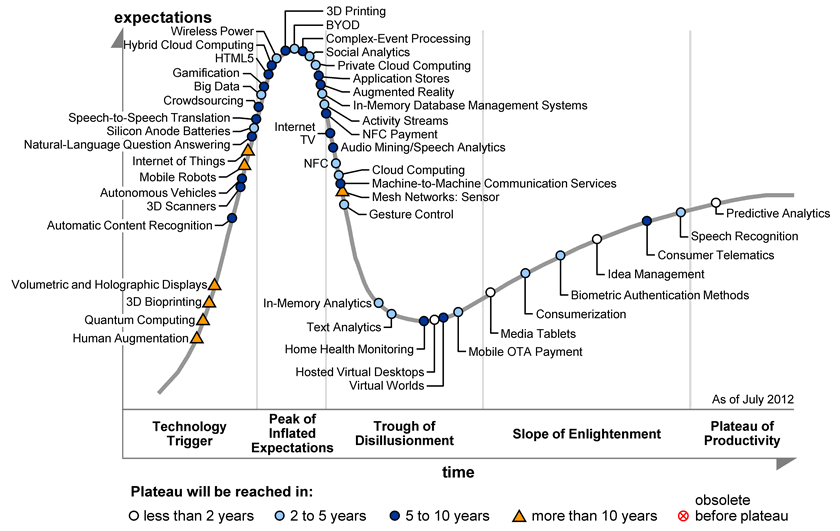
\includegraphics[width=0.8\linewidth]{./graphics/gartner.png}
\caption{Ciclo de Sobreexpectaci\'on de tecnolog{\'\i}as emergentes de \mbox{Gartner -- 2013 \cite{Gartner2013}.}}
\label{figure:gartner}
\end{figure}
%Figura Gartner

El dise\~no y la implementaci\'on de una interfaz mediante voz del usuario representa
una oportunidad, no solo para el estudio de esta \'area de investigaci\'on, sino para
demostrar la aplicabilidad del reconocimiento del habla a un problema real.

Habiendo mencionado previamente la potencial importancia del dominio de la aplicaci\'on
para una interfaz por voz del usuario, la elecci\'on de un programa de composici\'on musical
no pod{\'\i}a ser injustificada.
Existen investigaciones realizadas que relacionan a la m\'usica y el reconocimiento
del habla, en particular, orientadas al problema de recuperaci\'on de informaci\'on
\mbox{musical \cite{Goto2004Speech, Schuller2003Hybrid}}.
Sin embargo, resulta interesante explorar la utilizaci\'on del reconocimiento
del habla para la composici\'on musical. Este enfoque, en el cual un programa recibe comandos
sonoros y emite tambi\'en un resultado sonoro, podr{\'\i}a resultar incluso m\'as natural.

El programa de composici\'on musical controlado por voz es un medio para:

\begin{itemize}
	\item Explorar y experimentar con el reconocimiento del habla y las interfaces de usuario.
	\item Contrastar teor{\'\i}a y pr\'actica.
	\item Demostrar la factibilidad de la soluci\'on de un problema real utilizando el
	reconocimiento del habla.
\end{itemize}

%!TEX root = ../tesis.tex
\chapter{Soluci\'on Propuesta}
\label{sec:solucion}

Numerosas aplicaciones en el \'area del reconocimiento del habla han sido desarrolladas: \emph{Siri} \cite{AppleSiri}, \emph{Google Now} \cite{GoogleNow}, 
\emph{Dragon Naturally Speaking} \cite{DragonNaturallySpeaking}, etc. Cada una de estas
aplicaciones satisface distintos tipos de requerimientos establecidos por los usuarios finales. 

En el cap\'itulo anterior se presentó el desafío que supone el diseño de interfaces basadas 
en reconocimiento del habla, así como los requerimientos básicos de la aplicación a ser implementada como 
parte de este trabajo final de grado.

Este cap\'itulo presenta, justifica y eval\'ua la soluci\'on espec\'ifica al problema de implementar una interfaz
basada en reconomiento del habla para la aplicaci\'on escogida.


%!TEX root = ../tesis.tex

\section{Tecnolog\'ia a Utilizar}
\label{sec:tecnologia-utilizada}

Como se expone en la secci\'on~\ref{sec:problema-especifico}, se propone el dise\~no
de una interfaz para componer m\'usica utilizando la voz. Adem\'as, este trabajo 
opta por la metodolog\'ia de trabajo
de c\'odigo abierto, lo cual implica: 

\begin{itemize}
    \item Utilizar tecnolog\'ias de c\'odigo abierto para el desarrollo de la interfaz.
    \item Establecer un proceso de desarrollo transparente y abierto.
    \item Ofrecer la interfaz desarrollada, junto con su c\'odigo fuente, de manera libre 
        y gratuita para la comunidad de c\'odigo abierto.
\end{itemize}

La metodolog\'ia adoptada para implementar la interfaz permite utilizar un proyecto
existente como punto de partida, y as\'i dise\~nar e implementar una interfaz alternativa que permite
controlar la aplicaci\'on por comandos de voz. Adem\'as,
el hecho de incorporar una nueva interfaz, permite analizar
una de las motivaciones de la secci\'on~\ref{sec:motivacion}: un programa de composici\'on
musical, que recibe comandos sonoros y emite tambi\'en un resultado sonoro, podr\'ia ser
m\'as natural para el usuario. 

La interfaz desarrollada se denomina \emph{TamTam Listens} y se basa en tecnolog\'ias de c\'odigo abierto.
Toma como punto de partida la aplicaci\'on \emph{TamTam Edit} y para realizar el reconocimiento 
de comandos de voz utiliza los proyectos \emph{PocketSphinx} \cite{PocketSphinxHomePage} 
y \emph{Voxforge} \cite{Voxforge}.  A continuaci\'on se presentan los proyectos
utilizados como punto de partida para la soluci\'on implementada.

\subsection{TamTam Edit}
\label{sec:tamtam-edit}

La m\'usica es a menudo descrita como la forma m\'as pura de representaci\'on matem\'atica, es m\'as,
te\'oricos de la m\'usica han utilizado las matem\'aticas para resolver problemas musicales
\cite{TheSoundOfNumbers}. Esto sirvi\'o de inspiraci\'on para la creaci\'on del compendio de 
actividades\footnote{Una Actividad, es una aplicaci\'on en el entorno de escritorio \emph{Sugar}.}
conocido como \emph{TamTam} desarrollado para la computadora XO\footnote{La XO, es una computadora 
port\'atil de bajo costo y consumo desarrollada por el proyecto \gls{olpc}.},
con los siguientes objetivos:

\begin{itemize}
    \item Proveer a los ni\~nos un ambiente de informaci\'on cultural construyendo m\'usica y sonidos.
    \item Brindar una experiencia sonora/musical divertida para usuarios sin conocimientos musicales.
    \item Promover un camino hacia experiencias musicales m\'as sofisticadas.
    \item Promover un instrumento musical con su propio ``sonido''.
    \item Desarrollar un ambiente din\'amico y mutable que propone la simpleza y permite la complejidad.
    \item Favorecer la creaci\'on de m\'usica grupalmente.
    \item Introducir los conceptos musicales y otros como: programaci\'on y audio.
\end{itemize}

\emph{TamTam Edit} es una aplicaci\'on, que forma parte del conjunto de actividades musicales 
\emph{TamTam}, que proporciona una interfaz intuitiva para crear, modificar y organizar notas ubicadas 
en pistas virtuales.
Adem\'as incluye una paleta de casi cien tipos de sonidos y modelos de construcci\'on musical que permite 
crear distintos tipos de variaciones en estilos musicales \cite{TamTamWiki}.


Las secciones principales del programa se pueden observar en la figura~\ref{figure:ui-tamtam} 

\begin{figure}[H]
\centering
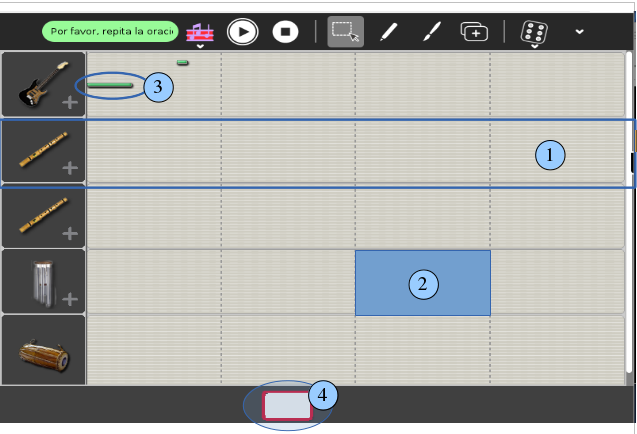
\includegraphics[width=0.8\textwidth]{./graphics/ui-tamtam-edit.png}
\caption{Interfaz de \emph{Tamtam Edit} y sus secciones principales}
\label{figure:ui-tamtam}
\end{figure}

Como se puede apreciar en la figura~\ref{figure:ui-tamtam}, la interfaz se encuentra organizada en 
cinco pistas y cada pista (1) tiene asociada un instrumento (la quinta pista esta reservada para
instrumentos de tipo bater{\'\i}a). Cada pista se divide en 4 
compases (del comp\'as uno al cuatro) y cada comp\'as (2) se divide en 12 tiempos (del uno al doce). 
Las notas (3) se dibujan en los compases, como se puede ver, la longitud de la nota indica su 
duraci\'on y su altura el tipo de nota. Adem\'as la aplicaci\'on esta organizada en partituras (4), que 
son como hojas de cuaderno, y son \'utiles para componer m\'usicas largas.

En general, la interacci\'on entre el usuario y \foreign{TamTam Edit} que se presenta en
la figura~\ref{figure:ui-tamtam} se realiza de modo tradicional.
El usuario utiliza el teclado y el rat\'on para interactuar con la aplicaci\'on a trav\'es de elementos
gr\'aficos como botones y men\'us. 

Este trabajo de grado busca incorporar un medio de interacci\'on alternativo al propuesto por \emph{TamTam Edit}. 
A continuaci\'on se presentan los motivos que determinaron la elecci\'on de esta aplicaci\'on como punto de partida:

\begin{itemize}
    \item Impacto social: \emph{TamTam Edit} es una aplicaci\'on que forma parte de la plataforma establecida
    por el proyecto \gls{olpc}, el cual busca potenciar el proceso educativo \cite{OLPC}. 
    Los ni\~nos con alg\'un tipo de discapacidad tienen a menudo problemas para utilizar una computadora mediante
    dispositivos perif\'ericos tradicionales como el mouse o el teclado.

    En estos casos, la posibilidad de operar esta actividad mediante la voz ser{\'\i}a de gran beneficio 
    para los ni\~nos, mejorando la accesibilidad de la plataforma, y generando por tanto un impacto social
    positivo importante.
    \item Naturalidad de interacci\'on: utilizar la voz para interactuar con una aplicaci\'on podr{\'\i}a
    ofrecer una mayor naturalidad con respecto al enfoque tradicional de interacci\'on, teniendo en cuenta
    que es el medio de interacci\'on entre las personas.
    \item No reinventar la rueda: como el objetivo es incorporar una interfaz basada en reconocimiento del
    habla a una aplicaci\'on, se elige \emph{TamTam Edit} para no construir la aplicaci\'on desde cero,
    sino extender las capacidades de una ya existente.
    \item C\'odigo abierto: el motivo anterior es posible gracias a que \emph{TamTam Edit} es un 
    proyecto de c\'odigo abierto, lo cual brinda a los desarrolladores la libertad de extender las 
    funcionalidades de la aplicaci\'on.
    \item Lenguaje de programaci\'on: la actividad se encuentra implementada en el lenguaje de 
    programaci\'on Python. La librer{\'\i}a de reconocimiento del habla a ser utilizada proporociona 
    \emph{bindings} 
    \footnote{Un \emph{binding} es un componente \emph{software}
   que permite hacer uso de las funcionalidades prove{\'\i}das por una librer{\'\i}a, implementada
    en un determinado lenguaje de programaci\'on, utilizando un lenguaje de programaci\'on diferente. 
    En este caso particular, \emph{Pocketsphinx} est\'a implementado en C y C++.} para 
    este lenguaje, lo cual supone una ventaja importante para la implementaci\'on de la interfaz.
\end{itemize}


\subsection{Voxforge}
\foreign{Voxforge} es un proyecto que busca recopilar grabaciones de voz de modo a crear 
y ofrecer varios corpus de habla bajo una licencia que permita su libre utilizaci\'on. 

A partir de estos corpus, es posible construir modelos ac\'usticos para su uso con motores de 
reconocimiento del habla de c\'odigo abierto, como \foreign{Pocketsphinx}.

\foreign{Voxforge} cuenta con grabaciones en diferentes idiomas, entre ellos ingĺ\'es, franc\'es, 
alem\'an y espa\~nol.


\subsection{PocketSphinx}

El cap\'itulo~\ref{sec:tecnologias} clasifica a las herramientas que permiten implementar soluciones
basadas en reconocimiento del habla en tres categor\'ias: Aplicaciones, \gls{api}s y Librer\'ias. 
Dada la naturaleza de este trabajo, se opta por elegir una librer\'ia para implementar la interfaz
alternativa a la ofrecida por \emph{TamTam Edit}.

Para la implementaci\'on de la interfaz operable a trav\'es de la voz se elige la librer\'ia 
\emph{PocketSphinx} que, como se menciona en la secci\'on~\ref{sec:pocketsphinx}, es un motor de 
reconocimiento del habla orientado a la optimizaci\'on del rendimiento y la portabilidad.

Uno de los objetivos espec\'ificos de este trabajo es aplicar y contrastar en la pr\'actica
los conocimientos te\'oricos adquiridos. Como indica la secci\'on~\ref{sec:librerias}, una librer\'ia es
el tipo de herramienta que requiere un conocimiento t\'ecnico espec\'ifico del \'area, adem\'as de
brindar una alta flexibilidad permitiendo al programador manipular los distintos componentes del
proceso de reconocimiento del habla. Por este motivo, una librer\'ia se considera la herramienta 
m\'as adecuada para cumplir el objetivo mencionado anteriormente.

A continuaci\'on se presentan los motivos t\'ecnicos que determinaron la elecci\'on de esta librer\'ia:

\begin{itemize}
    \item \emph{PocketSphinx} est\'a orientada a la optimizaci\'on del rendimiento, resultando adecuada 
    para sistemas con recursos limitados, como la computadora \emph{XO}.
    \item La librer\'ia es un proyecto de c\'odigo abierto, por lo tanto se cumple la metodolog\'ia 
    de trabajo adoptada.
    \item \emph{PocketSphinx} ofrece soporte \emph{offline}, lo cual permite su utilizaci\'on en ambientes
    sin conexi\'on a internet, como ocurre frecuentemente con las \emph{XO}.
    \item Existen \foreign{bindings} para el lenguaje de programaci\'on Python, lo cual hace muy 
    sencilla la tarea de utilizar la librer\'ia desde el c\'odigo Python.
\end{itemize}

\foreign{PocketSphinx} implementa el proceso del reconocimiento del habla basado en el enfoque 
estad{\'\i}stico, el cual se present\'o en el cap{\'\i}tulo~\ref{sec:proceso}. La librer{\'\i}a incluye
los diferentes algoritmos necesarios para las fases del proceso.

\begin{figure}[H] 
\centering
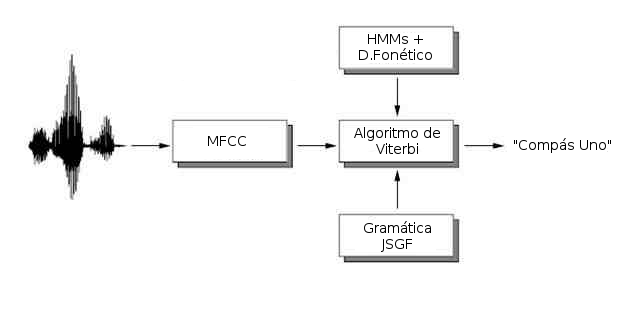
\includegraphics[width=0.8\textwidth]{./graphics/pocketsphinx.png}
\caption{Reconocimiento del habla mediante PocketSphinx. Gr\'afico basado en \cite{VerenichASR}.}
\label{figure:proceso-pocketsphinx}
\end{figure}

Como conjunto de caracter{\'\i}sticas espectrales, \foreign{Pocketsphinx} utiliza los coeficientes
espectrales en las frecuencias de mel (MFCC por sus siglas en ingl\'es).

En los \gls{hmm} del modelo ac\'ustico, utiliza mezclas Gaussianas para definir las probabilidades de 
transici\'on entre estados. El diccionario fon\'etico debe ser definido por el desarrollador.

Aunque \foreign{PocketSphinx} soporta modelos de lenguaje basados en n-gramas, para este trabajo 
se utiliza un modelo de lenguaje basado en gram\'atica. Esto se debe a la simpleza del lenguaje y a la 
falta de datos de entrenamiento para un modelo estad{\'\i}stico del mismo.

Como decodificador se utiliza el algoritmo de Viterbi, haciendo uso de la t\'ecnica de b\'usqueda en haz
para reducir el espacio de b\'usqueda.

\section{Tamtam Listens}
\label{sec:tamtam-listens}

La aplicación desarrollada, denominada \emph{Tamtam Listens}, es el resultado de la combinación
de las tecnolog\'ias mencionadas anteriormente. Por lo tanto, \emph{Tamtam Listens} representa una
interfaz de interacci\'on alternativa para la aplicaci\'on \emph{Tamtam Edit}.

El reconocimiento de los comandos de voz se implement\'o como un servicio de \emph{dbus}\cite{Dbus2013}, que es
un mecanismo para comunicaci\'on entre procesos de linux. Por lo tanto, el servicio puede ser utilizado
no solo por \emph{Tamtam Listens} si no por cualquier aplicaci\'on de linux. 

\emph{Pocketsphinx} requiere de un modelo ac\'ustico y un modelo de lenguaje para realizar
el reconocimiento de comandos. Para el modelo ac\'ustico se utiliz\'o el prove\'ido por el proyecto \emph{Voxforge}
\cite{Voxforge}, que es un proyecto que busca proveer modelos ac\'usticos para motores de reconocimientos
de c\'odigo abierto. Para el modelo de lenguaje se defini\'o una gram\'atica en formato \gls{jsgf} 
\cite{JSGF2000}, que permiti\'o definir los comandos soportados por la aplicaci\'on de una manera sencilla. 

\subsection{Gram\'atica}

A continuaci\'on se puede observar un fragmento de la gram\'atica \gls{jsgf} utilizada para definir 
los comandos soportados por \emph{Tamtam Listens}, m\'as adelante se presentar\'an los comandos
en forma de grafo para una mejor comprensi\'on.

\lstset{
  basicstyle=\scriptsize,        % the size of the fonts that are used for the code
  breakatwhitespace=false,         % sets if automatic breaks should only happen at whitespace
  frame=single,                    % adds a frame around the code
  language=Octave,                 % the language of the code
  numbersep=5pt,                   % how far the line-numbers are from the code
  showstringspaces=false,          % underline spaces within strings only
  stepnumber=2,                    % the step between two line-numbers. If it's 1, each line will be numbered
  tabsize=2                       % sets default tabsize to 2 spaces
}

\begin{figure}[H]
\begin{lstlisting}
#JSGF V1.0;
grammar tamtam;

public <tamtam-listens> = <comando> | <pagina> | <pista-a>     | <pista-b>  | 
                          <seleccionar-compas> | <crear-nota>  | <seleccionar-nota> | 
                          <duplicar-nota>      | <borrar-nota> | <volumen> | <tempo> | 
                          <configurar-nota>    | <loop>;

<comando>  = REPRODUCIR MUSICA  | PAUSAR MUSICA   | PARAR MUSICA | GENERAR MUSICA | 
             CREAR NUEVA MUSICA | EXPORTAR MUSICA | SALIR DE TAMTAM;
<pagina>   = ( CREAR NUEVA | DUPLICAR | LIMPIAR ) PARTITURA | PARTITURA <orden>;
<orden>    = ( ANTERIOR | SIGUIENTE );
<loop>     = (BASURA)+;
\end{lstlisting}
\caption{Fragmento de la gram\'atica utilizada en \emph{Tamtam Listens}}
\end{figure}

Los comandos pueden clasificarse en Generales (G), de Pista (P) y de Comp\'as (C). A continuaci\'on
se presentan los distintos comandos soportados, utilizando grafos para representarlos y as\'i facilitar
su comprensi\'on. El nodo coloreado hace referencia a la \'ultima palabra de un comando v\'alido para la aplicaci\'on

\subsubsection{Comandos Generales}

\begin{figure}[H] 
\centering
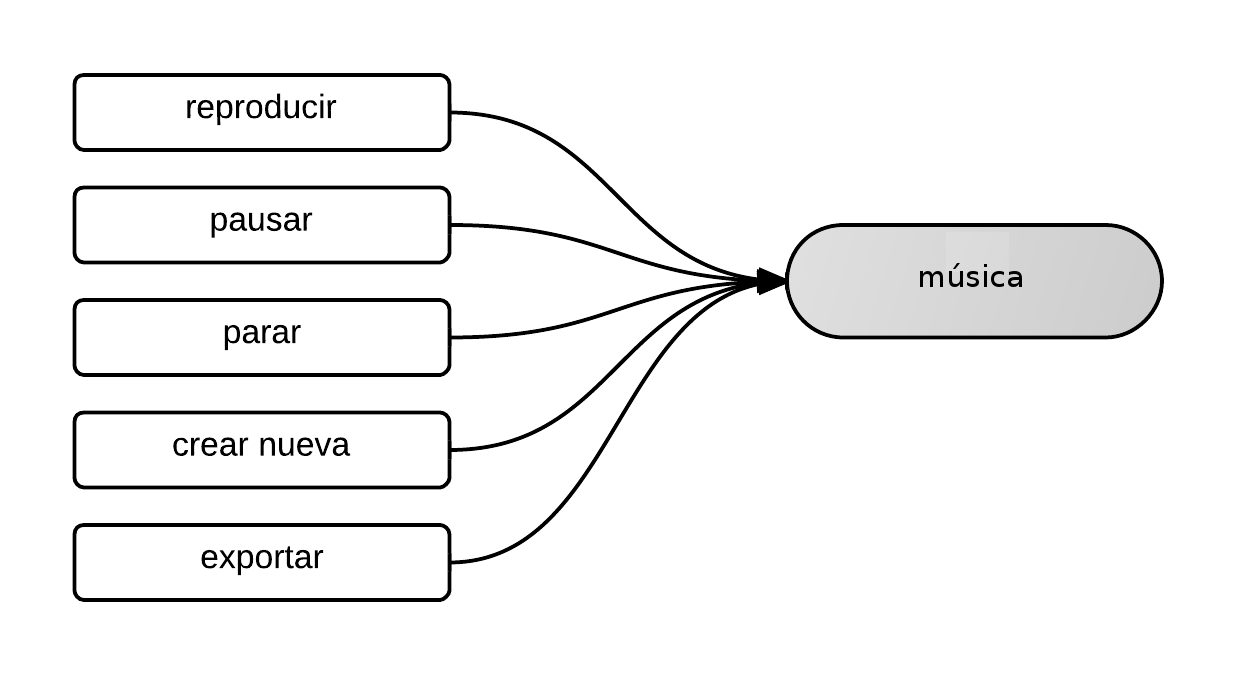
\includegraphics[width=0.5\textwidth]{./graphics/cmd-musica.png}
\caption{Comandos para reproducir, pausar, parar, exportar y crear una m\'usica}
\label{figure:cmd-crear-musica}
\end{figure}

\begin{figure}[ht]
\begin{minipage}[b]{0.5\linewidth}
\centering
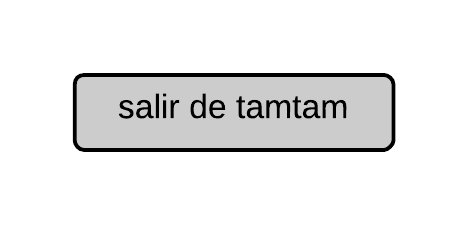
\includegraphics[width=0.6\linewidth]{./graphics/salir.png}
\caption{Comando para salir de la aplicaci\'on}
\label{figure:cmd-salir}
\end{minipage}
\quad
\begin{minipage}[b]{0.5\linewidth}
\centering
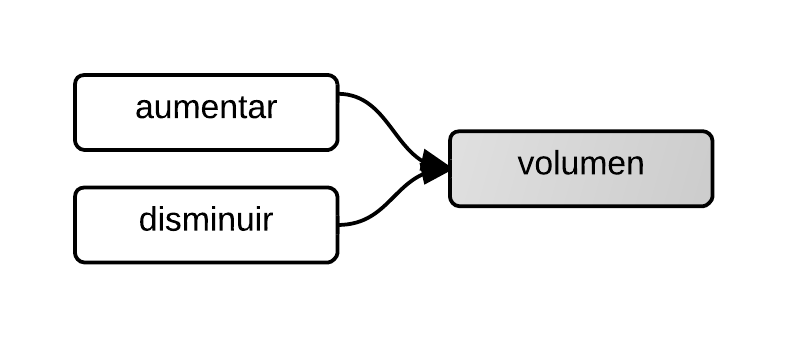
\includegraphics[width=0.6\linewidth]{./graphics/cmd-vol.png}
\caption{Comandos para aumentar/disminuir el volumen general}
\label{figure:cmd-vol}
\end{minipage}
\end{figure}


\begin{figure}[ht]
\begin{minipage}[b]{0.5\linewidth}
\centering
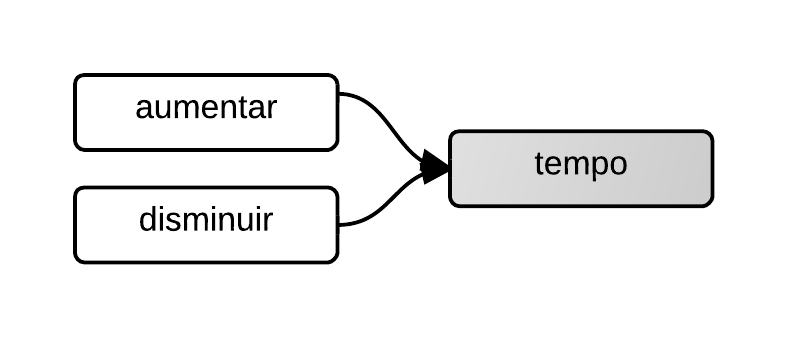
\includegraphics[width=0.6\linewidth]{./graphics/cmd-tempo.png}
\caption{Comandos para aumentar/disminuir el tempo general de al aplicaci\'on}
\label{figure:cmd-tempo}
\end{minipage}
\quad
\begin{minipage}[b]{0.5\linewidth}
\centering
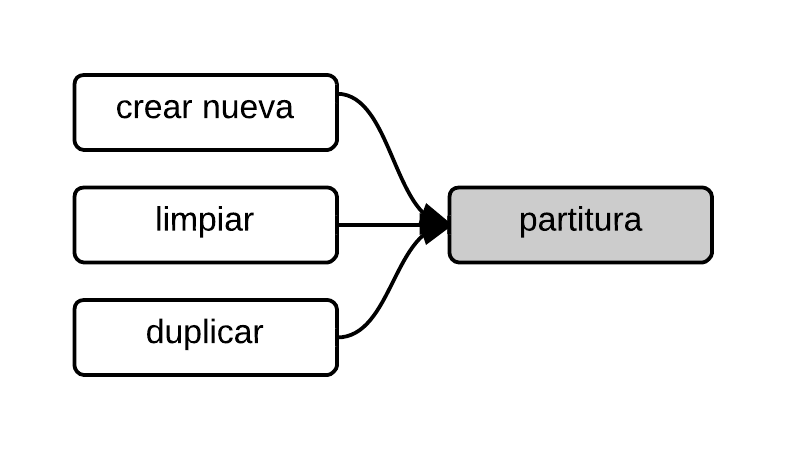
\includegraphics[width=0.6\linewidth]{./graphics/partitura-1.png}
\caption{Comandos para crear, limpiar y duplicar la partitura actual}
\label{figure:cmd-partitura-1}
\end{minipage}
\end{figure}


\begin{figure}[H]
\begin{minipage}[b]{0.5\linewidth}
\centering
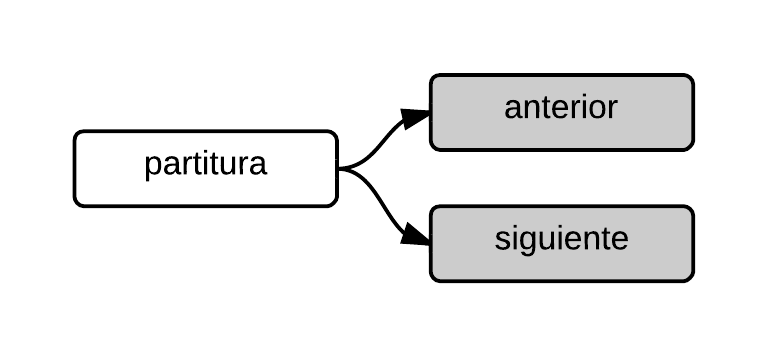
\includegraphics[width=0.6\linewidth]{./graphics/partitura-2.png}
\caption{Comandos para navegar entre partituras}
\label{figure:cmd-partitura-2}
\end{minipage}
\quad
\begin{minipage}[b]{0.5\linewidth}
\centering
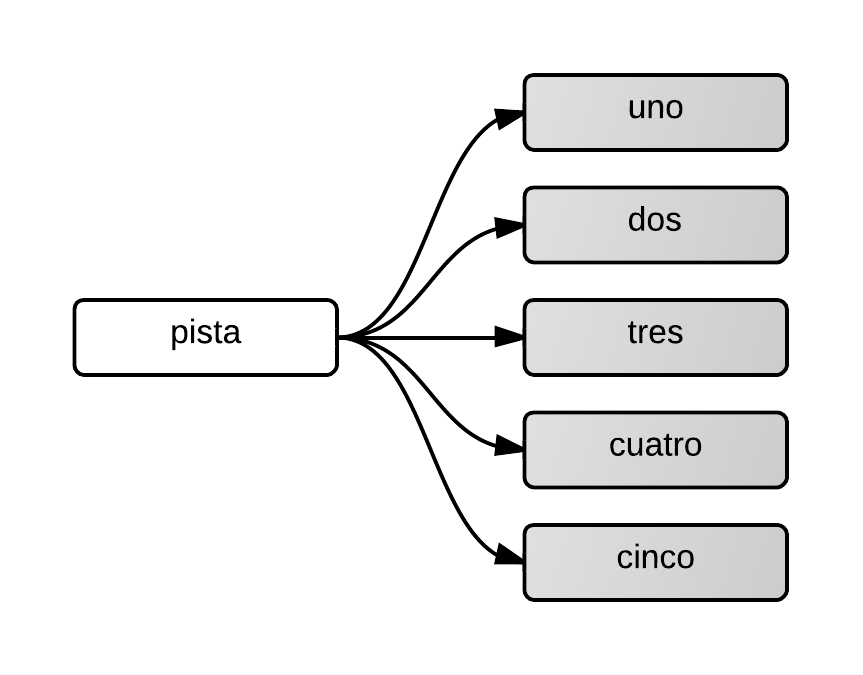
\includegraphics[width=0.6\linewidth]{./graphics/cmd-pista-1.png}
\caption{Comando para ubicarse en una pista}
\label{figure:cmd-partitura-1}
\end{minipage}
\end{figure}


\begin{figure}[H]
\begin{minipage}[b]{0.5\linewidth}
\centering
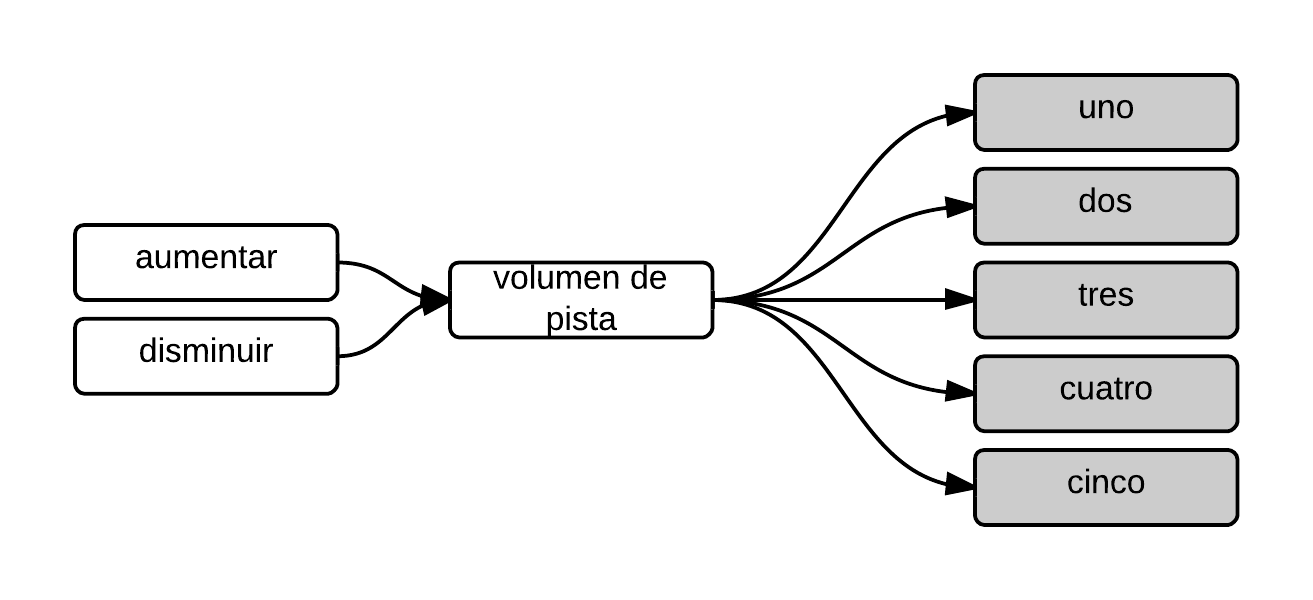
\includegraphics[width=0.8\linewidth]{./graphics/vol-pista.png}
\caption{Comandos para aumentar/disminuir el volumen de una pista en particular}
\label{figure:cmd-vol-pista}
\end{minipage}
\quad
\begin{minipage}[b]{0.5\linewidth}
\centering
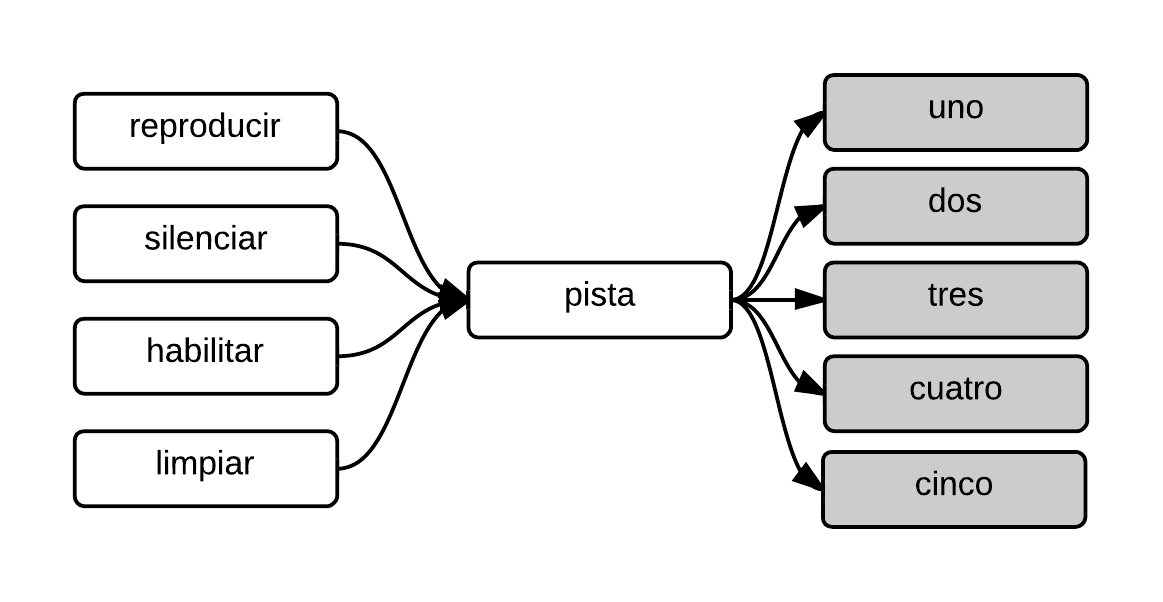
\includegraphics[width=0.9\linewidth]{./graphics/rep-pista.png}
\caption{Comandos para reproducir, silenciar, habilitar y limpiar una pista en particular}
\label{figure:cmd-rep-pista}
\end{minipage}
\end{figure}

\begin{figure}[H]
\centering
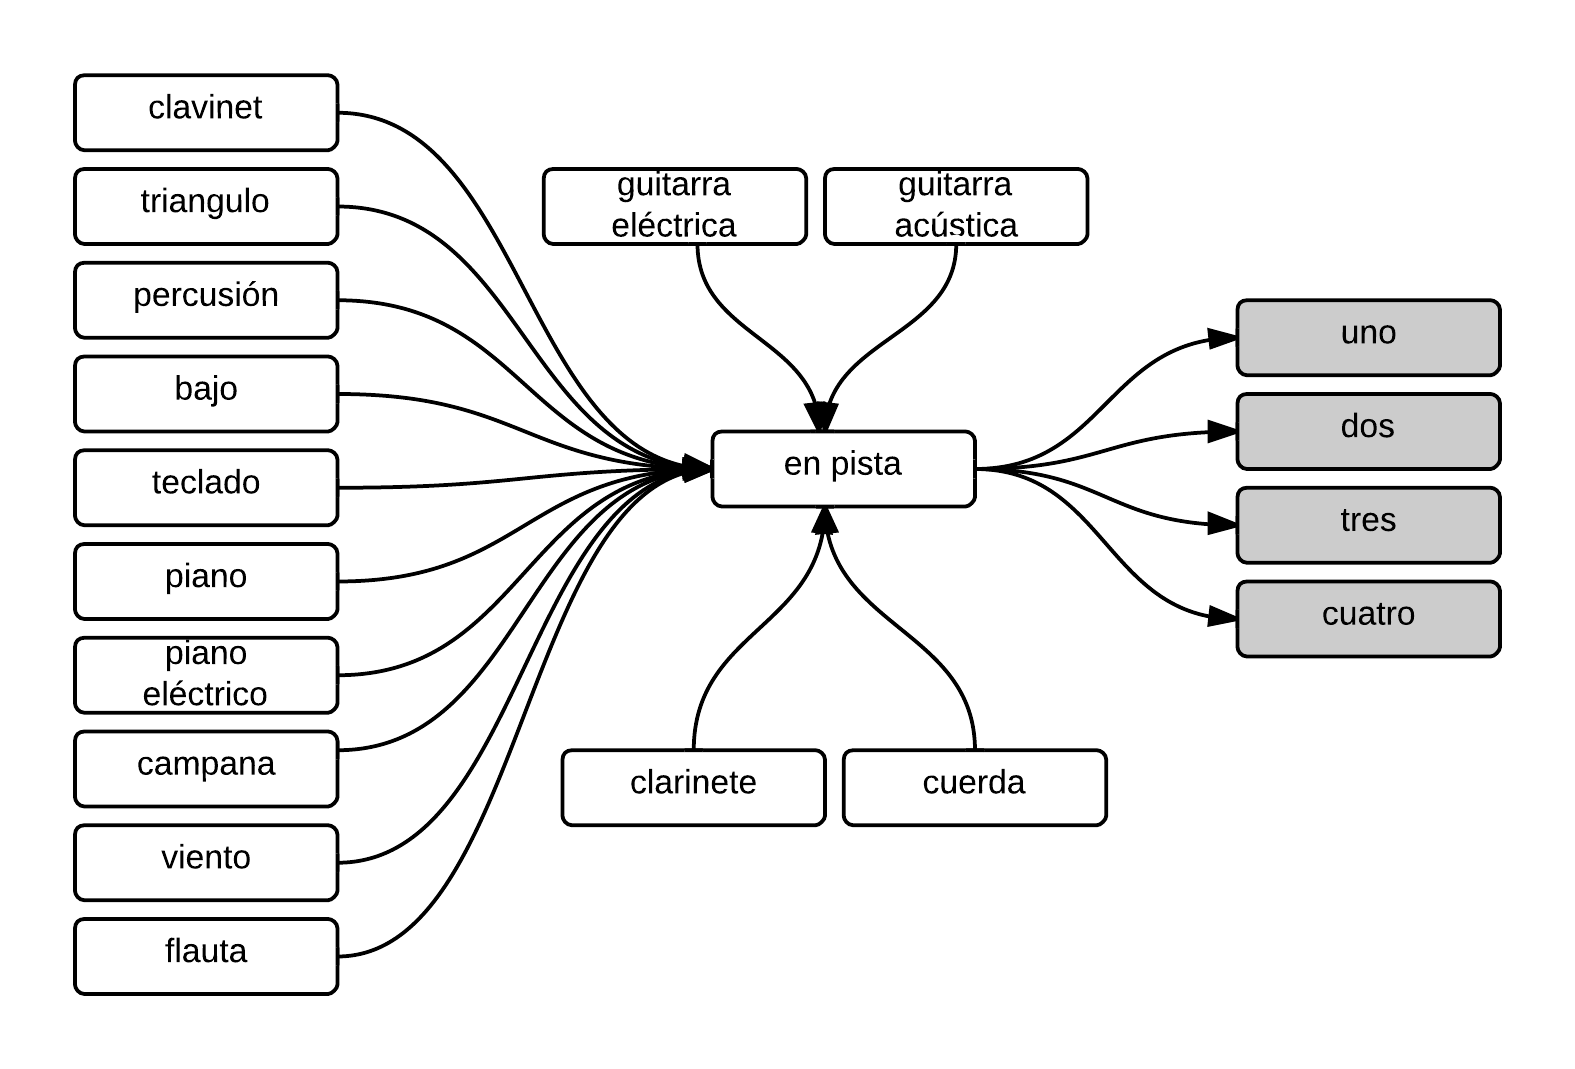
\includegraphics[width=0.8\textwidth]{./graphics/inst-p1-4.png}
\caption{Selecci\'on de instrumento para pistas del uno al cuatro}
\label{figure:cmd-inst-p1-4}
\end{figure}

\begin{figure}[H]
\begin{minipage}[b]{0.5\linewidth}
\centering
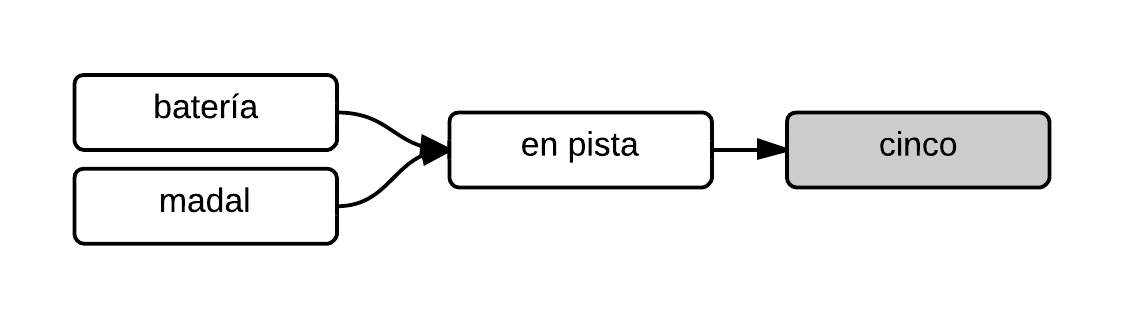
\includegraphics[width=1\linewidth]{./graphics/inst-p5.png}
\caption{Selecci\'on de instrumento para la pista cinco}
\label{figure:cmd-inst-p5}
\end{minipage}
\quad
\begin{minipage}[b]{0.5\linewidth}
\centering
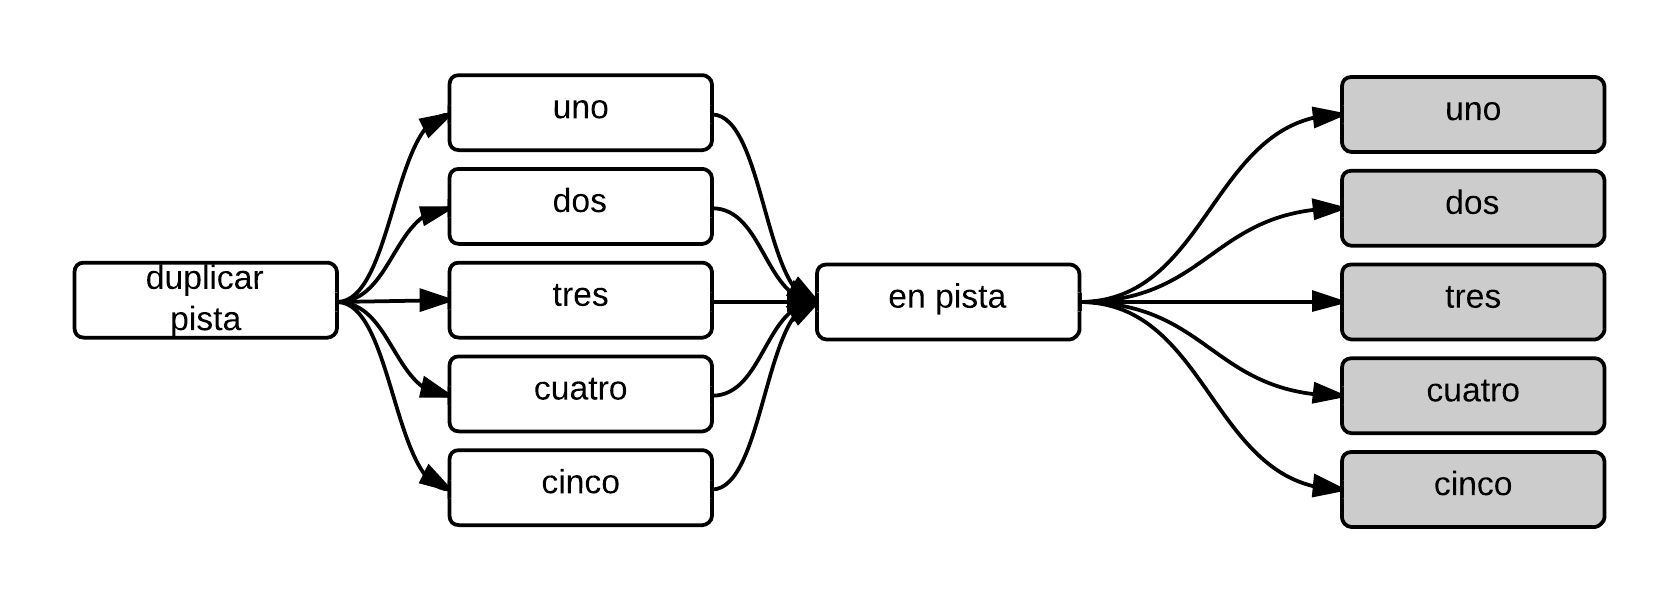
\includegraphics[width=1\linewidth]{./graphics/dup-pista.png}
\caption{Comando para duplicar las notas de una pista en otra}
\label{figure:cmd-dup-pista}
\end{minipage}
\end{figure}

\subsubsection{Comandos de Pista}

Este comando nos ubica dentro de una pista en particular. Por lo tanto, se debe
seleccionar una pista para poder utilizar este comando.

\begin{figure}[H]
\centering
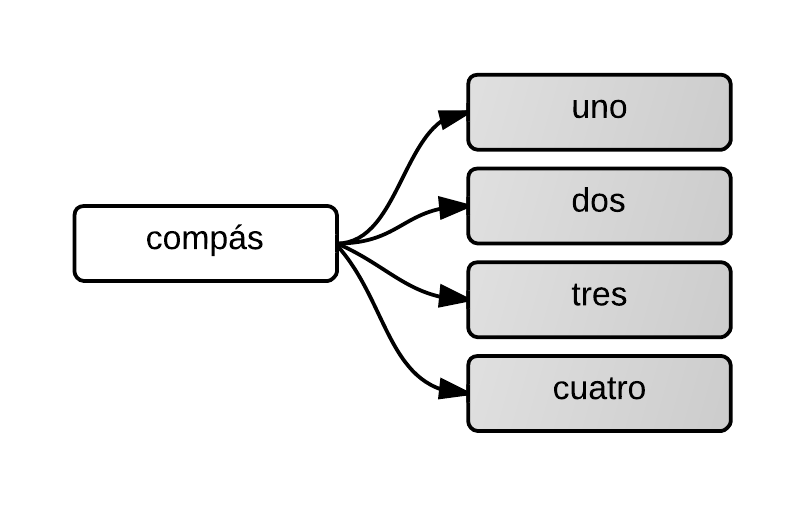
\includegraphics[width=0.4\linewidth]{./graphics/cmd-compas.png}
\caption{Comando para ubicarse en un comp\'as}
\label{figure:cmd-compas}
\quad
\end{figure}

\subsubsection{Comandos de Comp\'as}

Estos comandos son muy importantes para la aplicación ya que nos permiten crear, modificar, 
eliminar las notas musicales.

\begin{figure}[H]
\begin{minipage}[b]{0.5\linewidth}
\centering
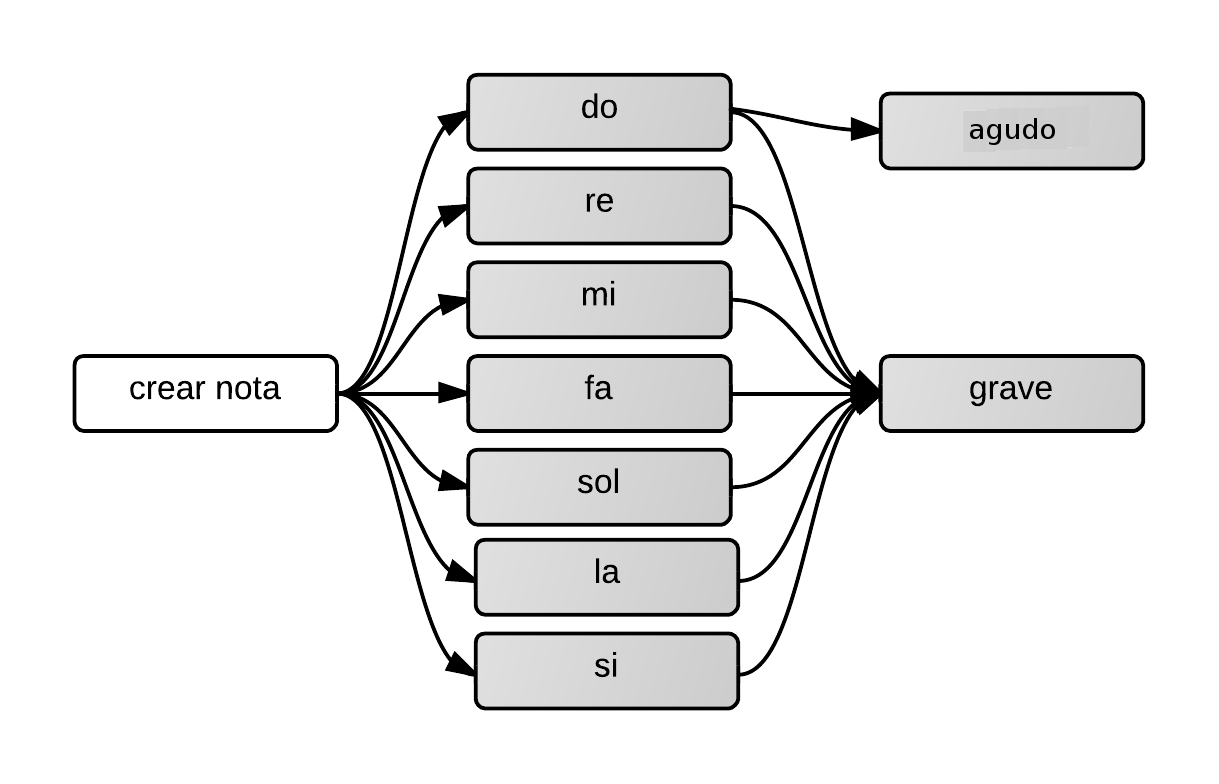
\includegraphics[width=1\linewidth]{./graphics/cmd-crear-nota.png}
\caption{Comando para crear una nota}
\label{figure:cmd-crear-nota}
\end{minipage}
\quad
\begin{minipage}[b]{0.5\linewidth}
\centering
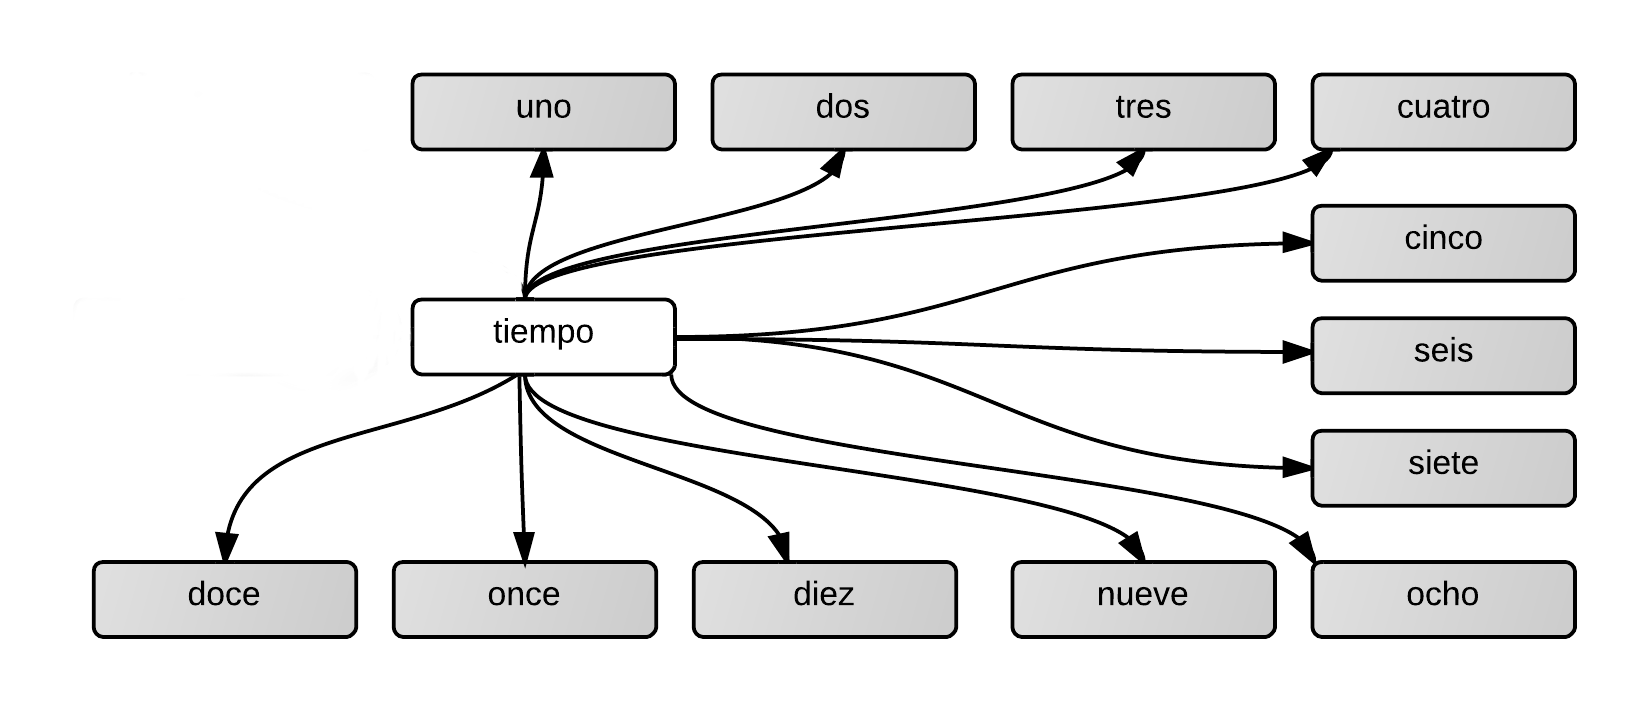
\includegraphics[width=1.1\linewidth]{./graphics/cmd-tiempo-compas.png}
\caption{Comando para ubicarse en un tiempo dado, dentro de un comp\'as}
\label{figure:cmd-tiempo-compas}
\end{minipage}
\end{figure}

\begin{figure}[H]
\begin{minipage}[b]{0.5\linewidth}
\centering
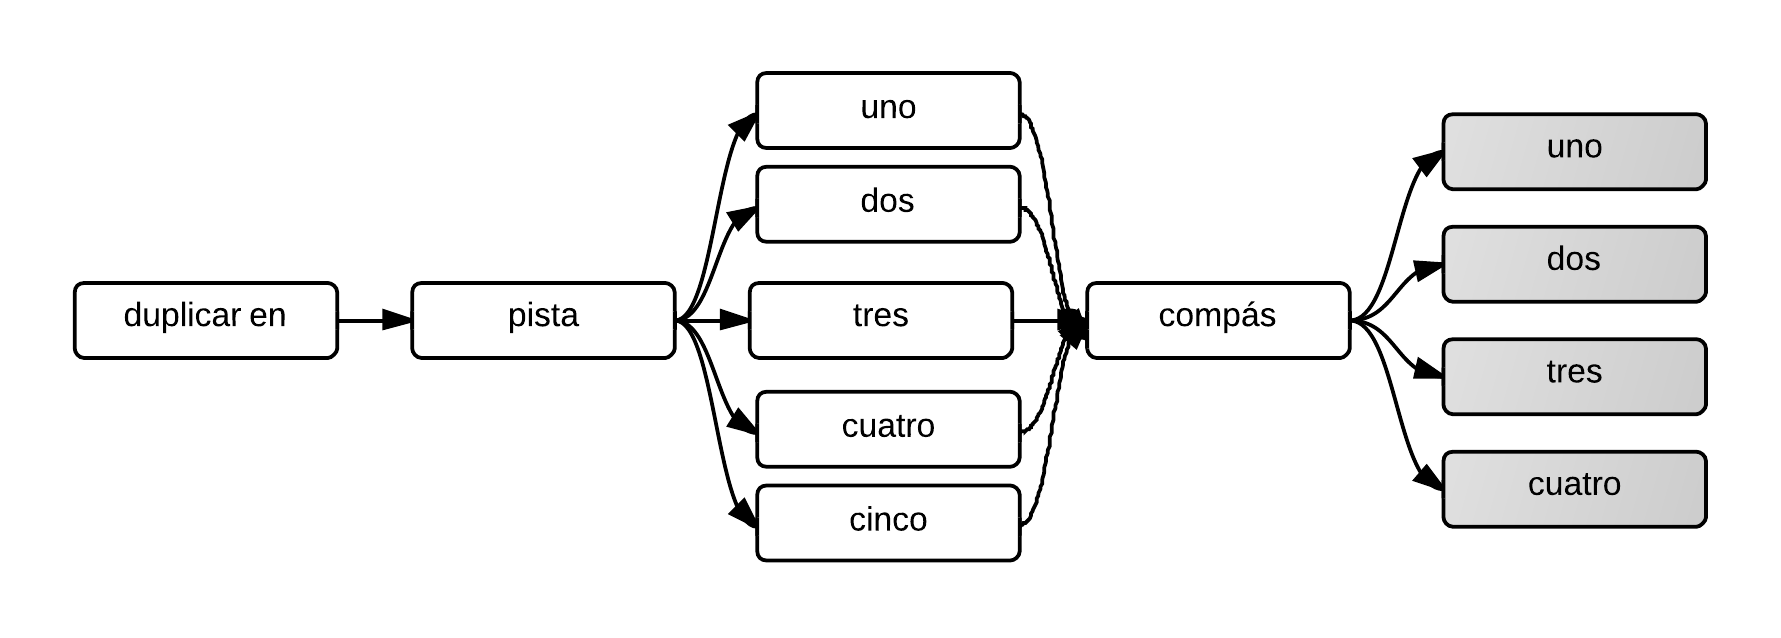
\includegraphics[width=1.2\linewidth]{./graphics/cmd-dup-nota.png}
\caption{Comando para duplicar una nota previamente seleccionada}
\label{figure:cmd-dup-nota}
\end{minipage}
\quad
\begin{minipage}[b]{0.5\linewidth}
\centering
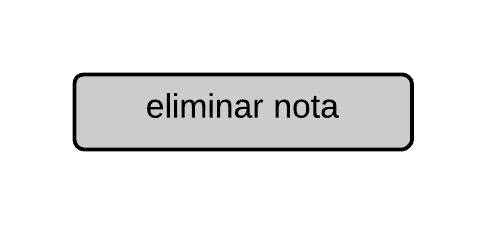
\includegraphics[width=0.5\linewidth]{./graphics/del-note.png}
\caption{Comando para eliminar un nota previamente seleccionada}
\label{figure:cmd-del-nota}
\end{minipage}
\end{figure}


\begin{figure}[H]
\begin{minipage}[b]{0.5\linewidth}
\centering
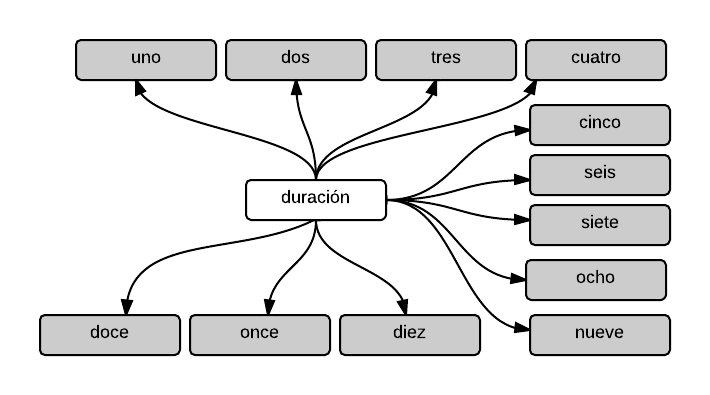
\includegraphics[width=0.9\linewidth]{./graphics/cmd-dur.png}
\caption{Comando que permite configurar la duraci\'on de una nota}
\label{figure:cmd-dur}
\end{minipage}
\quad
\begin{minipage}[b]{0.5\linewidth}
\centering
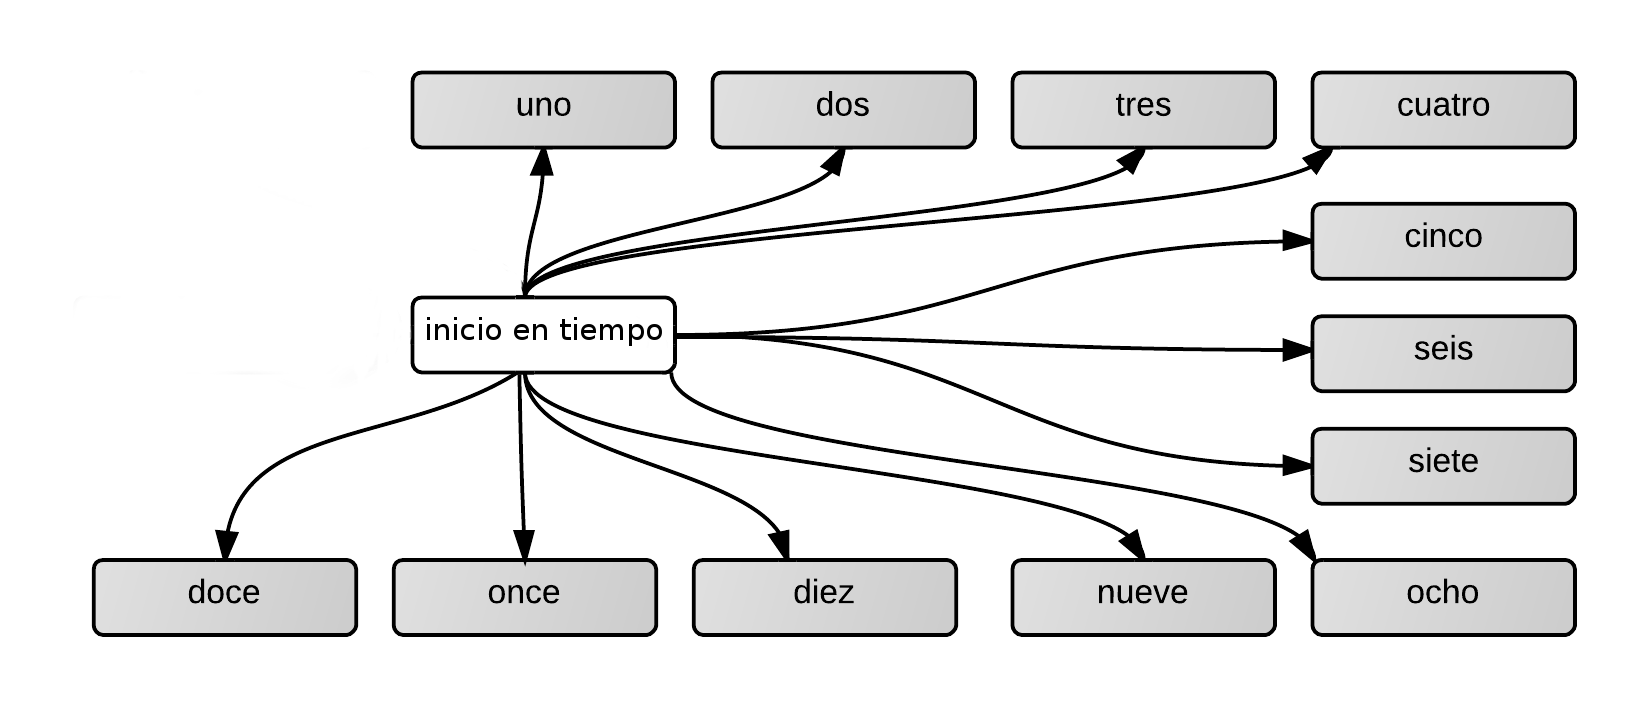
\includegraphics[width=1.1\linewidth]{./graphics/cmd-note-tiempo.png}
\caption{Comando que permite configurar el inicio de una nota dentro del comp\'as}
\label{figure:cmd-note-tiempo}
\end{minipage}
\end{figure}


\subsection{Diccionario}

Otro elemento requerido por \emph{Pocketsphinx} es el diccionario, que permite mapear
palabras a secuencia de fonemas. En la siguiente figura se muestra un fragmento del diccionario
utilizado por la aplicaci\'on.

\begin{figure}[H]
\begin{lstlisting}
REPRODUCIR RR E P R O D U S I R
PAUSAR P A U S A R
PARAR  P A R A R
GENERAR  J E N E R A R
PARTITURA P A R T I T U R A
SIGUIENTE S I G I E N T E
ANTERIOR A N T E R I O R
\end{lstlisting}
\caption{Fragmento del diccionario utilizad en \emph{Tamtam Listens}}
\end{figure}

La combinaci\'on de estos componentes es lo que permite a \emph{Pocketsphinx} realizar el
reconocimiento de los comandos de voz.


%!TEX root = ../tesis.tex
\chapter{Evaluaci\'on}
\label{sec:evaluacion}


% introduccion
En el cap{\'\i}tulo anterior se describi\'o la soluci\'on propuesta para el estudio de interfaces basadas en
reconocimiento del habla, la cual fue implementada como parte de este trabajo de grado.

Con el fin de realizar una evaluaci\'on tanto de la aplicaci\'on misma como de ciertos conceptos 
e hip\'otesis planteados, se plantea la realización de una prueba de usabilidad. 
Como parte de la misma, se miden y analizan factores relacionados a la aplicaci\'on,
al usuario y a la interacci\'on entre ambos.

Este cap{\'\i}tulo presenta los principales aspectos de dise\~no del estudio propuesto: objetivos, metodolog{\'\i}a
y m\'etricas utilizadas. La \'ultima secci\'on describe con mayor detalle el an\'alisis con respecto
a uno de los factores estudiados, el error humano.


%!TEX root = ../tesis.tex
\section{Objetivos}
\label{sec:objetivos-estudio}

Fueron definidos los siguientes objetivos para el estudio realizado:

\begin{itemize}
	\item Evaluar experimentalmente la aplicaci\'on desarrollada, teniendo en cuenta 
	aspectos t\'ecnicos y funcionales.
	\item Identificar problemas que se presentan al utilizar una interfaz mediante voz y,
	 de ser posible, sugerir posibles soluciones.
	\item Proponer criterios que puedan utilizarse para la evaluaci\'on de interfaces 
	mediante voz.
	\item Verificar y validar la utilidad de los criterios propuestos, de acuerdo a 
	la informaci\'on y las conclusiones que pueden obtenerse mediante los mismos.
	\item Analizar la correlación entre los factores medidos, de modo a identificar
	posibles relaciones entre los mismos. 
	\item Obtener conclusiones relacionadas a factores externos a la aplicaci\'on, 
	como la memoria del usuario y el tiempo de entrenamiento previo.
\end{itemize}
%!TEX root = ../tesis.tex
\section{Metodolog{\'\i}a}
\label{sec:metodolog{\'\i}a}
A continuaci\'on se describen brevemente distintos aspectos relacionados al
estudio realizado.

\subsection{Muestra}
Las pruebas fueron realizadas con 12 usuarios, estudiantes de Ingenier{\'\i}a Inform\'atica
de la Facultad Polit\'ecnica, Universidad Nacional de Asunci\'on. Ninguno de los usuarios 
hab{\'\i}a utilizado anteriormente la aplicaci\'on evaluada, de manera a evitar los efectos
de la experiencia previa.

La cantidad de sujetos de prueba fue elegida de acuerdo a la recomendaci\'on realizada
en \cite{Hwang:2010} para este tipo de estudios. Adem\'as, de acuerdo a \cite[p.~267]{Rubin2008}, 
este n\'umero es el necesario de modo a obtener resultados estad{\'\i}sticos significativos.

\subsection{Duraci\'on}
Cada sesi\'on de pruebas tuvo una duraci\'on aproximada de una hora.
Las sesiones fueron realizadas a lo largo de 2 semanas.

\subsection{Ambiente de Pruebas}
De modo a realizar el estudio en un ambiente controlado, todas las sesiones fueron
realizadas en un Laboratorio de Inform\'atica de la Facultad Poĺit\'ecnica. Esto
permiti\'o minimizar los efectos de la interferencia sonora y humana durante el
desarrollo de las pruebas.

\subsection{Roles}
Cada sesi\'on cont\'o con 3 participantes:
	\begin{itemize}
		\item Facilitador: responsable de administrar los distintos pasos del estudio, explicarlos al usuario 
		y aclarar las dudas que se presenten durante la fase inicial. 
		\item Observador: responsable de tomar nota de los eventos que sucedan durante las pruebas, principalmente
		tiempo de inicio y fin de cada paso y otros sucesos que aporten valor al estudio (errores, preguntas, etc.).
		\item Usuario: persona sin conocimientos del sistema. Los detalles del aprendizaje y primeras interacciones
		(tareas) con la aplicaci\'on se registran para su posterior an\'alisis.	
	\end{itemize}

\subsection{Test de Memoria}
Previamente a la realizaci\'on de las tareas, se llev\'o a cabo un test de memoria del usuario, basado en
el Test de Aprendizaje Auditivo Verbal de Rey \cite{Lopez1998}. 

Para la prueba, el facilitador le{\'\i}a una lista
de 15 palabras al usuario, luego de lo cual este \'ultimo deb{\'\i}a repetir aquellas que recordaba.
El proceso se repet{\'\i}a 5 veces en total, registr\'andose las palabras que el usuario recordaba y el orden en que
lo hac{\'\i}a.

\subsection{Entrenamiento}
La fase de entrenamiento tuvo como objetivo la introducci\'on del usuario a los distintos comandos por voz disponibles
para interactuar con TamTam Listens. 
Para evitar la influencia de las variaciones que pod{\'\i}an haberse presentado en una
explicaci\'on directa del facilitador al usuario, fue grabada una serie de videotutoriales que se presentaban al usuario
en esta etapa.
Adem\'as, cada usuario recibi\'o una copia del manual de la aplicaci\'on, el cual describ{\'\i}a en mayor detalles las
funcionalidades de la aplicaci\'on.

\subsection{Tareas}
Cada usuario realiz\'o un total de 4 tareas durante la prueba de usabilidad:
	\begin{itemize}			
		\item Tareas 1 y 2: tareas simples y breves que buscan llevar a la pr\'actica los conceptos aprendidos en los
		videotutoriales. Se realizan con ayuda del facilitador y el manual de aplicaci\'on.
		\item Tarea 3: tarea un poco m\'as compleja, la cual se realiza ya sin asistencia del facilitador. El usuario puede, sin embargo, consultar el manual de aplicaci\'on.
		\item Tarea 4: tarea de mayor dificultad, la cual se realiza sin asistencia del facilitador ni el manual de
		aplicaci\'on. El resultado de esta tarea, si se lleva a cabo correctamente, es una sencilla pieza musical.
	\end{itemize}

\subsection{Encuesta de Usabilidad}
Luego de finalizadas las tareas, los usuarios completaron una breve encuesta relacionada a la usabilidad de
la aplicaci\'on y a las interfaces por voz de usuario en general.
Se recogi\'o la opini\'on de los usuarios con respecto a las palabras y comandos utilizados, la duraci\'on del
entrenamiento y su predisposici\'on a utilizar interfaces de usuario basadas en el habla. Las respuestas se
registraron utilizando una escala de Likert \cite{Allen:2007}.
Adem\'as, en cada punto, se solicitaron sugerencias de parte del usuario. 	

\subsection{Recopilaci\'on y An\'alisis de Datos} 
Al finalizar cada sesi\'on, se recopilaron los siguientes datos:
	\begin{itemize}			
		\item Registro de resultados del test de memoria.
		\item Registro de las notas del observador.
		\item Grabaci\'on de las tareas realizadas por el usuario.
		\item Encuesta completada por el usuario.
	\end{itemize}

Una vez finalizadas todas las pruebas, se procedi\'o a la sumarizaci\'on y an\'alisis de los datos disponibles
a partir de estos materiales. Los factores que se tuvieron en cuenta en esta etapa se describen en la
siguiente secci\'on.


%!TEX root = ../tesis.tex
\section{Factores Analizados}
\label{sec:factores}

Esta secci\'on describe los factores que se tienen en cuenta para el \'analisis a realizarse
en base a los datos recopilados a partir de las pruebas de usabilidad.
Se definen tambi\'en las m\'etricas utilizadas para la cuantificaci\'on de cada factor estudiado.

\subsection{Memoria del Usuario}
\label{sec:memoria-del-usuario}
Factor relacionado a la capacidad de retenci\'on de informaci\'on del usuario.
Se considera interesante su an\'alisis debido a que:
\begin{itemize}
	\item TamTam Listens se trata de una aplicaci\'on completamente nueva para el usuario.
	\item Los comandos de voz deben ser memorizados por el usuario para la interacci\'on con
	la apliaci\'on.
\end{itemize}
\subsubsection{M\'etrica Utilizada}
La memoria del usuario se midie a trav\'es de los resultados del test de memoria que se lleva
a cabo con cada usuario como parte de la prueba de usabilidad.
El resultado del test de memoria administrado es la cantidad de palabras, de un total de 15,
que el usuario consigue recordar al cabo de 5 repeticiones, siendo 12--13 el resultado promedio
esperado. El resultado del test de memoria se representa como $M$.

\subsection{Correctitud de la aplicaci\'on}
Factor relacionado al comportamiento esperado por parte de un sistema de reconocimiento del
habla. Se busca responder a la pregunta: {?`}Qu\'e tan correctamente se reconocen los comandos 
del usuario?
Los valores de las m\'etricas relacionadas a la correctitud de la aplicaci\'on se calculan
en base a las tareas 3 y 4, por realizarse estas sin asistencia del facilitador.  
\subsubsection{M\'etricas Utilizadas}
\begin{itemize}
	\item Tasa de Aciertos de Comandos: se considera que el sistema reconoce correctamente
	un comando, si el usuario efectivamente ha pronunciado el mismo.

	La tasa de aciertos es la raz\'on entre la cantidad de comandos correctamente reconocidos 
	y la cantidad de comandos correctamente pronunciados por el usuario. 
	La misma se representa como $A$.
	
	Sean:

	\begin{itemize}
		\item $r_{ij}$ n\'umero de reconocimientos correctos del \mbox{comando $i$} pronunciado por el usuario $j$,
		por parte de la aplicaci\'on.
		\item $c_{ij}$ n\'umero de pronunciaciones correctas del \mbox{comando $i$} por parte del usuario $j$.
	\end{itemize}
	La tasa de aciertos del comando $i$ para el usuario $j$ se define como: 

	\begin{equation*}
		a_{{comando}_{ij}}=\frac{r_{ij}}{c_{ij}}
	\end{equation*}


	Sea $N_{j}$ la cantidad total de comandos diferentes pronunciados (correcta o incorrectamente) por el usuario $j$,
	la tasa de aciertos para el usuario  se define como:
	
	\begin{equation*}
		A=a_{{usuario}_j}=\frac{\sum_k^{N_{j}}a_{{comando}_{kj}}}{N_{j}}
	\end{equation*}

	La tasa de aciertos del sistema se obtiene hallando el promedio de los valores correspondientes
	a cada usuario.

	\item Tasa de Error de Comandos: es la raz\'on entre la cantidad de comandos correctos no reconocidos 
	y la cantidad de comandos correctamente pronunciados por el usuario. 
	La misma se representa como $E_1$ y es igual a $1-A$.

\end{itemize}

\subsection{Error Humano}
Factor relacionado a las equivocaciones por parte del usuario en su interacci\'on con
TamTam Listens.
Un comando se considera err\'oneo o incorrecto por parte del usuario si:
\begin{itemize}
	\item El usuario no respeta el orden de las palabras: esto es, pronuncia las palabras de un comando en el orden incorrecto.
	\item El usuario se confundie entre dos comandos: esto es, utiliza palabras correspondientes a m\'as
	de un comando.
	\item El usuario junta dos o m\'as comandos: esto es, pronuncia de una sola vez dos o m\'as comandos.
	\item El usuario duda mientras pronuncia el comando: esto es, titubea o repite una palabra del comando.
	\item El usuario utiliza comandos incompletos: esto es, pronunciando solo algunas palabras del comando.
	\item El usuario utiliza palabras que no forman parte del lenguaje.
	\item El usuario viola alguna otra regla impuesta por el lenguaje de la aplicaci\'on.
\end{itemize}
Los valores de las m\'etricas relacionadas al error humano se calculan
en base a las tareas 3 y 4, por realizarse estas sin asistencia del facilitador. 

\subsubsection{M\'etricas Utilizadas}
\begin{itemize}
	\item Cantidad de Errores: sumatoria de errores por usuario, clasificados en
	alguno de los tipos previamente mencionados. Se representa como $E_2$.
	\item Tasa de Error Humano: se define como la raz\'on entre la cantidad de comandos incorrectos
	y la cantidad de comandos pronunciados. Se representa como $E_3$.
	
	Sean:

	\begin{itemize}
		\item $p_{ij}$ n\'umero de pronunciaciones incorrectas del \mbox{comando $i$} por parte del usuario $j$.
		\item $t_{ij}$ n\'umero de pronunciaciones (correctas e incorrectas) del \mbox{comando $i$} por parte del usuario $j$.
	\end{itemize}
	La tasa de error humano del comando $i$ para el usuario $j$ se define como: 

	\begin{equation*}
		e_{{comando}_{ij}}=\frac{p_{ij}}{t_{ij}}
	\end{equation*}

	El c\'alculo de la tasa de error humano de cada usuario se lleva a cabo de forma an\'aloga 
	a la tasa de aciertos.
\end{itemize}

\subsection{Eficiencia}
Factor relacionado al grado de productividad que logra el usuario de la aplicaci\'on.
\subsubsection{M\'etricas Utilizadas}
\begin{itemize}
	\item Duraci\'on de Tareas Uno y Dos: es la suma del tiempo que le toma al usuario
	terminar la tarea 1 ($T_1$) y el que le toma terminar la tarea 2 ($T_2$). 
	Estas tareas se realizan con asistencia por parte del facilitador. 
	La duraci\'on se midi\'o en minutos. Se representa como $T_{1+2}$.
	\item Duraci\'on de Tareas Tres y Cuatro: es la suma del tiempo que le toma al usuario
	terminar la tarea 3 ($T_3$) y el que le toma terminar la tarea 4 ($T_4$). 
	Estas tareas se realizan sin asistencia por parte del facilitador. 
	La duraci\'on se mide en minutos. Se representa como $T_{3+4}$.
	\item Cantidad de Comandos Utilizados: es la cantidad total de comandos diferentes utilizados
	al menos una vez por el usuario durante las tareas 3 y 4. Se representa como $U$.
	\item Correctitud de la Tarea Cuatro: para \'el c\'alculo de esta medida, se descompone la
	\'ultima tarea en lo distintos pasos necesarios para completarla correctamente.
	De esta manera, la tarea cuatro se considera compuesta por 72 elementos:
	\begin{itemize}
		\item Creaci\'on de 54 notas.
		\item Selecci\'on de 4 instrumentos.
		\item Cambios en la duraci\'on de 12 notas.
		\item Reproducci\'on de la m\'usica.
		\item Exportaci\'on de la m\'usica.
	\end{itemize}
	La correctitud de la tarea 4 para cada usuario se define como la raz\'on entre la cantidad de operaciones
	correctamente realizadas y el total de operaciones (72). Se representa como $C$.
\end{itemize}

\subsection{Satisfacci\'on del Usuario}
Factor relacionado a la apreciaci\'on subjetiva del usuario sobre su interacci\'on con la aplicaci\'on y
las interfaces basadas en reconocimiento del habla en general.
\subsubsection{M\'etricas Utilizadas}
La opini\'on del usuario se mide a trav\'es de los resultados de la encuesta que se realiza como parte de
la prueba de usabilidad, posterior a la finalizaci\'on de las tareas. Las respuestas se
registran utilizando una escala de Likert \cite{Allen:2007} con valores del 1 al 7.

Se solicita la opini\'on del usuario con respecto a:
\begin{itemize}
	\item Que tan adecuadas son palabras utilizadas.
	\item Que tan adecuados son los comandos utilizados.
	\item Que tan adecuada resulta la duraci\'on del entrenamiento.
	\item Que tan frecuentemente utilizar{\'\i}a las interfaces por voz del usuario.
\end{itemize}

Posteriormente, de modo a eliminar el potencial efecto de los estilos de respuesta
de los usuarios \cite{Fischer2010}, se utiliza el m\'etodo de estandarizaci\'on 
por rango \cite{Pagolu2011} para reescalar los resultados de la encuesta.

Siendo:
\begin{itemize}
	\item $min_i$ la respuesta de menor valor del usuario $i$.
	\item $max_i$ larespuesta de mayor valor del usuario $j$.
\end{itemize}

Para cada respuesta $s$ del usuario $i$, el valor ajustado $s_a$ se define como:

\begin{equation*}
s_a=\frac{s-min_i}{max_i-min_i}
\end{equation*}


De esta manera, todas las respuestas pasan a estar en el rango entre 0 y 1.  





%!TEX root = ../tesis.tex
\section{An\'alisis del Error Humano}
\label{sec:evaluacionError}
Todas las m\'etricas presentadas en la secci\'on anterior se calcularon para cada usuario,
pudiendo promediarse para obtener un valor representativo de la aplicaci\'on.

En el caso particular del error humano, se realiz\'o un estudio m\'as detallado
por considerarse que podr{\'\i}a llevar a obtener conclusiones interesantes. De esta manera,
se calcularon tambi\'en:

\begin{itemize}
	\item Tasa de Error Humano por Longitud del Comando: la longitud de un comando se define
	como la cantidad de palabras que lo componen. La longitud de los comandos disponibles en el 
	lenguaje de TamTam Listens va de 2 a 6 palabras.

	El c\'alculo de la tasa de error se llev\'o a cabo para cada longitud posible.  


	\item Tasa de Error Humano por Nivel Contextual del Comando: el nivel contextual de un comando
	se define de acuerdo al contexto en que se aplica el mismo.
	Para TamTam Listens, se definieron 3 niveles posibles:
		\begin{itemize}
			\item General: comandos que afectan la m\'usica en general. 

			Ejemplo: Crear Nueva M\'usica.
			\item Pista: comandos que dependen de una pista seleccionada para su aplicaci\'on. 

			Ejemplo: Piano en Pista 2.
			\item Comp\'as: comandos que que dependen de una pista y un comp\'as seleccionados 
			para su aplicaci\'on. 

			Ejemplo: Crear Nota Do.
		\end{itemize}
	
		
	El c\'alculo de la tasa de error se llev\'o a cabo para cada nivel contextual posible.
	\item Distribuci\'on del Error Humano con respecto al Tiempo transcurrido: para cada usuario, 
	se dividi\'o $T_{3+4}$ en 10 etapas (de 10\%¸de la duraci\'on cada una).

	Para cada etapa se calcul\'o el porcentaje de errores cometidos, con respecto al total de
	errores cometidos por el usuario ($E_2$).

	La distribuci\'on del error humano con respecto al tiempo transcurrido se obtuvo calculando 
	el promedio de los valores de los usuarios para cada etapa.  
\end{itemize}
%!TEX root = ../tesis.tex
\chapter{Resultados Obtenidos}
\label{sec:resultados}

En este cap\'itulo se exponen los resultados de las pruebas de usuarios descritas en el cap\'itulo
anterior. Los
distintos valores obtenidos para las variables consideradas ser\'an presentados de manera tabular, dichos
valores ser\'an analizados para identificar correlaciones.


\section{Test de Memoria}

Una de las primeras actividades de la prueba de usabilidad fue el Test de Memoria ($M$), en la tabla~\ref{sec:tabla-memoria}
se puede ver el desempe\~no de cada sujeto en esta actividad.

\begin{table}[H]
\centering
\footnotesize
\begin{tabular}{|p{1.6cm}|p{1.6cm}|}
\hline
    Sujeto & $M$ \\
    \hline 
    1 & 14 \\
    2 & 10 \\
    3 & 14 \\
    4 & 11 \\
    5 & 8 \\
    6 & 14 \\
    7 & 13 \\
    8 & 12 \\
    9 & 14 \\
    10 & 14 \\
    11 & 15 \\
    12 & 14 \\
\hline
Promedio &  12,75 \\
\hline
\end{tabular}
\caption{Resumen del Test de Memoria}
\label{sec:tabla-memoria}
\end{table}

Como se mencion\'o en la secci\'on~\ref{sec:memoria-del-usuario}, 12 a 13 palabras recordadas es el promedio esperado. Esto
se puede comprobar observando el valor de la \'ultima fila de la tabla~\ref{sec:tabla-memoria}.
 
\section{Entrenamiento}

Luego del Test de Memoria cada sujeto realiz\'o dos tareas simples de manera tal a poder 
llevar a la pr\'actica los conocimientos te\'oricos aprendidos.
A continuaci\'on la tabla~\ref{sec:tabla-t1-memoria} presenta el tiempo $T_{1+2}$ de
cada sujeto, siendo $T_{1+2}$ la suma del tiempo de la tarea uno y dos (en minutos) acampa\~nado
de los resultados del test de memoria; la \'ultima fila de la tabla corresponde al promedio de los valores
presentados.

\begin{table}[H]
\centering
\footnotesize
\begin{tabular}{|p{1.6cm}|p{1.6cm}|p{1.6cm}|}
\hline
    Sujeto & $M$ & $T_{1+2}$ \\
    \hline 
    1 & 14 & 10,65 \\
    2 & 10 & 19,68 \\
    3 & 14 & 10,88 \\
    4 & 11 & 16,02 \\
    5 & 8 & 18,97 \\
    6 & 14 & 14,6 \\
    7 & 13 & 11,5 \\
    8 & 12 & 7,02 \\
    9 & 14 & 15,27 \\
    10 & 14 & 7,15 \\
    11 & 15 & 12,92 \\
    12 & 14 & 21,42 \\
\hline
    Promedio &  12,75 & 13,84  \\
\hline
\end{tabular}
\caption{Resumen del Test de memoria y tiempo $T1$ de cada sujeto}
\label{sec:tabla-t1-memoria}
\end{table}

Una vez terminadas las dos tareas iniciales cada sujeto realiz\'o dos tareas m\'as sin ayuda del facilitador.

\section{Tarea Tres}

La tarea tres es la primera de las dos tareas que el sujeto realiz\'o sin asistencia del facilitador, como
se explic\'o anteriormente, el sujeto tuvo la posibilidad de consultar el manual durante esta actividad.
A continuaci\'on la tabla~\ref{sec:tabla-tarea3} presenta las distintas variables consideradas con relaci\'on
a la tarea tres: Tasa de Aciertos ($A$), Error de la M\'aquina ($E_1$),  
Tasa de Error Humano ($E_2$), Duraci\'on ($T_3$), Cantidad de Errores ($E_3$) y Cantidad de Comandos Utilizados ($U$).

\begin{table}[H]
\centering
\footnotesize
\begin{tabular}{|p{1.6cm}|p{1.6cm}|p{1.6cm}|p{1.6cm}|p{1.6cm}|p{1.6cm}|p{1.6cm}|p{1.6cm}|}
\hline
    Sujeto &  $A$     & $E_1$    & $E_2$   & $T_3$      & $E_3$ & $M$ & $U$ \\
    \hline 
    1      & 53,42  & 46,58  & 2,83 & 0:10:39 & 4  & 14      &  28 \\
    2      & 68,46  & 31,54  & 5,96 & 0:10:28 & 11 & 10      &  26 \\
    3      & 90,99  & 9,01   & 4,11 & 0:07:14 & 9  & 14      &  28 \\
    4      & 66,84  & 33,16  & 0,81 & 0:16:52 & 1  & 11      &  31 \\
    5      & 93,47  & 6,53   & 3,08 & 0:12:53 & 3  & 8       &  30 \\
    6      & 81,17  & 18,83  & 3,06 & 0:09:04 & 3  & 14      &  30 \\
    7      & 86,86  & 13,14  & 6,48 & 0:05:04 & 4  & 13      &  27 \\
    8      & 95,15  & 4,85   & 5,17 & 0:05:00 & 2  & 12      &  29 \\
    9      & 95,61  & 4,39   & 9,23 & 0:12:31 & 9  & 14      &  28 \\
    10     & 87,32  & 12,68  & 6,51 & 0:05:26 & 8  & 14      &  32 \\
    11     & 84,70  & 15,30  & 1,79 & 0:10:58 & 5  & 15      &  28 \\
    12     & 95,53  & 4,47   & 9,55 & 0:12:05 & 18 & 14      &  37 \\
\hline
  Promedio & 83,29   & 19,59 & 4,88 & 0:09:51 & 6,17 & 12,75 & 29,5   \\
\hline
\end{tabular}
\caption{Resumen de las variables relacionadas con la tarea tres}
\label{sec:tabla-tarea3}
\end{table}

\section{Tarea Cuatro}

La tarea cuatro es la \'ultima tarea realizada por el sujeto. Como se mencion\'o anteriormente, es la tarea
de mayor dificultad ya que el sujeto la realiza sin ning\'un tipo de asistencia. A continuaci\'on se presenta
la tabla~\ref{sec:tabla-tarea4} que resume la tarea cuatro, incluyendo las variables presentadas en la tarea tres y, adem\'as, se
agrega la variable que mide la correctitud de la tarea cuatro ($C$)

\begin{table}[H]
\centering
\footnotesize
\begin{tabular}{|p{1.4cm}|p{1.4cm}|p{1.4cm}|p{1.4cm}|p{1.4cm}|p{1.4cm}|p{1.4cm}|p{1.4cm}|p{1.4cm}|}
\hline
Sujeto& $A$ & $E_1$ & $E_2$  & $T_4$      & $E_3$ & $C$ &  $M$ & $U$ \\
 \hline 
1  &  71,06 & 28,94 &  0     &  0:06:47   &  0  &  58,33  & 14 &  20  \\ 
2  &  73,23 & 26,77 &  3,80  &  0:13:34   &  8  &  91,67  & 10 &  22 \\
3  &  93,25 & 6,75  &  2,38  &  0:06:17   &  0  &  94,44  & 14 &  21 \\
4  &  68,07 & 31,93 &  6,05  &  0:16:55   &  5  &  69,44  & 11 &  22 \\
5  &  90,84 & 9,16  &  18,05 &  0:10:53   &  26 &  100      & 8  &  23 \\
6  &  74,38 & 25,62 &  3,51  &  0:09:10   &  1  &  91,67  & 14 &  19  \\
7  &  87,79 & 12,21 &  3,21  &  0:04:54   &  2  &  100      & 13 &  20  \\
8  &  83,87 & 16,13 &  7,47  &  0:06:47   &  4  &  100      & 12 &  22  \\
9  &  91,67 & 8,33  &  15    &  0:05:53   &  12 &  100      & 14 &  20  \\
10 &  88,57 & 11,43 &  2,78  &  0:03:40   &  2  &  70,83  & 14 &  18  \\
11 &  94,17 & 5,83  &  0     &  0:07:02   &  1  &  100      & 15 &  22  \\
12 &  93,43 & 6,57  &  9,92  &  0:10:11   &  7  &  73,61  & 14 &  29  \\
\hline
  Promedio & 84,19   & 15,80 & 6,01 & 0:08:30 & 5,67 & 87,5  &  12,75 & 21,5   \\
\hline
\end{tabular}
\caption{Resumen de las variables relacionadas con la tarea cuatro}
\label{sec:tabla-tarea4}
\end{table}

 
\section{Resumen}

Finalmente, se presenta la tabla que resume (por usuario) la prueba de usabilidad realizada. En la tabla~\ref{sec:tabla-resumen-prueba}
se pueden observar todas las m\'etricas juntas, la cual sirve como entrada 
para el analisis de correlaci\'on a realizar.

\begin{table}[H]
\centering
\footnotesize
\begin{tabular}{|p{1.2cm}|p{1.2cm}|p{1.2cm}|p{1.2cm}|p{1.2cm}|p{1.2cm}|p{1.2cm}|p{1.2cm}|p{1.2cm}|p{1.2cm}|}
\hline
Sujeto  &   $A$  &   $E_1$ &  $E_2$  &  $T_{1+2}$  & $T_{3+4}$     & $E_3$ & $C$ &  $M$ & $U$ \\
\hline 
1 &  58,25 & 41,75 & 2,20  & 10,65 & 17,43 & 4  & 58,33 & 14 & 36 \\
2 &  70,01 & 29,99 & 6,12  & 19,68 & 24,03 & 19 & 91,67 & 10 & 39 \\
3 &  93,73 & 6,27  & 2,75  & 10,88 & 13,52 & 9  & 94,44 & 14 & 40 \\
4 &  66,35 & 33,65 & 3,27  & 16,02 & 33,78 & 6  & 69,44 & 11 & 41 \\
5 &  93,32 & 6,68  & 9,42  & 18,97 & 23,77 & 29 & 100     & 8  & 43 \\
6 &  79,97 & 20,03 & 3,46  & 14,6  & 18,23 & 4  & 91,67 & 14 & 38 \\
7 &  87,62 & 12,38 & 4,98  & 11,5  & 9,97  & 6  & 100     & 13 & 38 \\
8 &  90,45 & 9,55  & 7,48  & 7,02  & 11,78 & 6  & 100     & 12 & 42 \\
9 &  93,49 & 6,51  & 13,14 & 15,27 & 18,4  & 21 & 100     & 14 & 38 \\
10 & 87,64 & 12,36 & 5,12  & 7,15  & 9,1   & 7  & 70,83 & 14 & 41 \\
11 & 89,32 & 10,68 & 1,22  & 12,92 & 18      & 6  & 100     & 15 & 41 \\
12 & 94,30 & 5,70  & 11,79 & 21,42 & 22,27 & 25 & 73,61 & 14 & 51 \\
\hline
\end{tabular}
\caption{Resumen de las variables de la prueba de usabilidad}
\label{sec:tabla-resumen-prueba}
\end{table}

De manera tal a poder tener un resumen general, se muestra en la tabla~\ref{sec:tabla-resumen-promedio} el promedio
de los valores expuestos anteriormente.

\begin{table}[H]
\centering
\footnotesize
\begin{tabular}{|p{1.2cm}|p{1.2cm}|p{1.2cm}|p{1.2cm}|p{1.2cm}|p{1.2cm}|p{1.2cm}|p{1.2cm}|p{1.2cm}|}
\hline
$A$  &   $E_1$ &  $E_2$  &  $T_{1+2}$  & $T_{3+4}$     & $E_3$ & $C$ &  $M$ & $U$ \\
\hline 
83,70 & 16,30 & 5,91 & 13,83  & 18,35  & 11,83 & 87,5  & 12,75  & 40.67 \\
\hline
\end{tabular}
\caption{Resumen General de las variables de la prueba de usabilidad}
\label{sec:tabla-resumen-promedio}
\end{table}

\section{Correlaci\'on}

A partir de los valores en la tabla~\ref{sec:tabla-resumen-prueba} y utilizando el \emph{Coeficiente de 
Correlaci\'on de Pearson}\cite{BoslaughStatistics2008} se llev\'o a cabo un an\'alisis  para identificar posibles
correlaciones entre las variables consideradas. El coeficiente de Pearson es una medida del grado de 
correlaci\'on lineal o dependencia entre dos variables $X$ e $Y$. El valor del coeficiente se encuentra entre
-1 y 1 inclusive. El valor -1 indica que las variables est\'an correlacionadas negativamente 
(cuando $X$ crece, $Y$ decrece y viceversa), 0 indica que no existe correlaci\'on y 1 que existe una correlaci\'on
positiva (cuando $X$ crece, $Y$ crece).

En la tabla que se muestra a continuaci\'on se pueden visualizar los coeficientes de correlaci\'on entre las m\'etricas estudiadas.

\begin{table}[H] 
\centering
\footnotesize
\begin{tabular}{|p{1.2cm}|p{1.2cm}|p{1.2cm}|p{1.2cm}|p{1.2cm}|p{1.2cm}|p{1.2cm}|p{1.2cm}|p{1.2cm}|p{1.2cm}|}
\hline
&  $A$  &   $E_1$ &  $E_2$  &  $T_{1+2}$  & $T_{3+4}$     & $E_3$ & $C$ &  $M$ & $U$ \\
\hline
$A$  &  1  &  -1  &  0,51  &  0,14  &  -0,09  &  0,69  &  0,5  &  0,22  &  0,53 \\
$E_1$  &  -1  &  1  &  -0,51  &  -0,14  &  0,09  &  -0,69  &  -0,5  &  -0,22  &  -0,53 \\
$E_2$  &  0,51  &  -0,51  &  1  &  0,4  &  0,23  &  0,71  &  0,29  &  -0,38  &  0,35  \\
$T_{1+2}$  &  0,14  &  -0,14  &  0,4  &  1  &  0,87  &  0,57  &  -0,04  &  -0,31  &  0,25 \\
$T_{3+4}$  &  -0,09  &  0,09  &  0,23  &  0,87  &  1  &  0,37  &  -0,16  &  -0,42  &  0,2 \\
$E_3$  &  0,69  &  -0,69  &  0,71  &  0,57  &  0,37  &  1  &  0,28  &  -0,29  &  0,52 \\
$C$  &  0,5  &  -0,5  &  0,29  &  -0,04  &  -0,16  &  0,28  &  1  &  -0,08  &  0,13 \\
$M$  &  0,22  &  -0,22  &  -0,38  &  -0,31  &  -0,42  &  -0,29  &  -0,08  &  1  &  -0,23 \\
$U$  &  0,53  &  -0,53  &  0,35  &  0,25  &  0,2  &  0,52  &  0,13  &  -0,23  &  1 \\
\hline
\end{tabular}
\caption{Coeficientes de correlaci\'on para las m\'etricas consideradas.}
\label{sec:tabla-correlacion}
\end{table}

Como se puede observar, existen correlaciones entre alguna de las m\'etricas presentadas, 
siendo algunas positivas y otras negativas. A continuaci\'on se listan algunas correlaciones identificadas:

\begin{itemize}
    \item $A$ y $E_2$, 0,51 correlaci\'on positiva fuerte
    \item $A$ y $E_3$, 0,69 correlaci\'on positiva fuerte
    \item $A$ y $C$, 0,50 correlaci\'on positiva fuerte
    \item $A$ y $U$, 0,53 correlaci\'on positiva fuerte
    \item $E_1$ y $U$, -0,53 correlaci\'on negativa fuerte
    \item $E_2$ y $C$, -0,50 correlaci\'on negativa fuerte
    \item $E_2$ y $T_{1+2}$, 0,40 correlaci\'on positiva fuerte
    \item $E_2$ y $U$, 0,35 correlaci\'on positiva moderada
    \item $E_2$ y $M$, -0,38 correlaci\'on negativa moderada
    \item $T_{1+2}$ y $T_{3+4}$, 0,87 correlaci\'on positiva muy fuerte
    \item $T_{1+2}$ y $M$, -0,31 correlaci\'on negativa moderada
    \item $T_{1+2}$ y $E_3$, 0,57 correlaci\'on positiva fuerte
    \item $T_{3+4}$ y $E_3$, 0,37 correlaci\'on positiva moderada
    \item $T_{3+4}$ y $M$, -0,42 correlaci\'on negativa fuerte
    \item $E_3$ y $U$, 0,52 correlaci\'on positiva fuerte
\end{itemize}


\section{An\'alisis del Error Humano}
\label{sec:resultados-error-humano}

En esta secci\'on se presentan las tasas de errores de acuerdo a factores que se consideran importantes debido
al tipo de aplicaci\'on desarrollada. 

\subsection{Tasa de Error Humano por Longitud del Comando}
El primer caso considerado es la tasa error con respecto a la longitud del comando
utilizado. En la tabla~\ref{sec:error-longitud} se pueden observar los valores obtenidos, las columnas
representan las distintas longitudes de comandos disponibles en la aplicaci\'on

\begin{table}[H]
\centering
\footnotesize
\begin{tabular}{|p{1.6cm}|p{1.6cm}|p{1.6cm}|p{1.6cm}|p{1.6cm}|p{1.6cm}|}
\hline
    Sujeto & 2 & 3 & 4 & 5 & 6  \\
    \hline 
    1 & 5,36   & 0     & 3,33  &0   &0 \\
    2 & 8,11   & 8,85  & 4,76  &0   &0 \\
    3 & 8,57   & 10,20 & 0 &  0  &33,33 \\
    4 & 3,08   & 3,64 & 0  & 0  & 0 \\
    5 & 2,94   & 18,18 & 8,33 &  0 & 77,77 \\
    6 & 2,08   & 2,5 & 0 & 0 & 20 \\
    7 & 5,26   & 6,90 & 0 & 0 & 0 \\
    8 & 2,78   & 0 & 13,33 & 40 & 16,67 \\
    9 & 7,55   & 11,63 & 40  &  62,5  & 20 \\
    10 & 5,13  & 2,5  & 18,75  &  0 & 60 \\
    11 & 0     & 4,35 & 0 & 20 & 66,67 \\
    12 & 20,19 & 1,52 & 6,25 & 0  & 63,64 \\
\hline
\end{tabular}
\caption{Tasa de Error Humano por Longitud del Comando}
\label{sec:error-longitud}
\end{table}

En la siguiente tabla se puede observar un resumen de la tabla anterior, de manera tal a poder presentar
el error a nivel general.

\begin{table}[H]
\centering
\footnotesize
\begin{tabular}{|p{1.6cm}|p{1.6cm}|p{1.6cm}|p{1.6cm}|p{1.6cm}|}
\hline
    2 & 3 & 4 & 5 & 6  \\
    \hline 
    6,96 & 5,68 & 7,46 & 14,81 & 42,11 \\
    \hline
\end{tabular}
\caption{Resumen de la Tasa de Error Humano por Longitud del Comando}
\label{sec:error-longitud-resumen}
\end{table}


\subsection[Tasa de Error Humano por Nivel Contextual del Comando]
{Tasa de Error Humano por Nivel Contextual del \\ Comando}

Se considera tambi\'en en el an\'alisis la tasa de error humano con respecto al contexto del comando, es decir
qu\'e tan dependiente es el comando utilizado con respecto a uno dicho previamente. 
En la tabla~\ref{sec:error-contexto} se pueden observar los valores para este factor.

\begin{table}[H]
\centering
\footnotesize
\begin{tabular}{|p{1.6cm}|p{1.6cm}|p{1.6cm}|p{1.6cm}|}
\hline
    Sujeto & General & Pista & Comp\'as \\
    \hline
1 & 1,32  & 50     & 0,94 \\
2 & 16,88 & 0      & 3,39 \\
3 & 13,95 & 0      & 7,55 \\
4 & 2,60 & 0      & 3,15 \\
5 & 31,25 & 0      & 5,41 \\
6 & 7,02 & 25     & 0 \\
7 & 10     & 0      & 2,67 \\
8 & 9,76 & 0      & 3,28 \\
9 & 21,74 & 0      & 16,42 \\
10 & 15     & 12,5 & 3,70 \\
11 & 10,91 & 0      & 0 \\
12 & 18,18 & 0      & 15,15 \\
    \hline
\end{tabular}
\caption{Tasa de Error Humano por Nivel Contextual del Comando}
\label{sec:error-contexto}
\end{table}

Al igual que el factor anterior, se muestra la versi\'on resumida del error en la 
tabla~\ref{sec:error-contexto-resumen}

\begin{table}[H]
\centering
\footnotesize
\begin{tabular}{|p{1.6cm}|p{1.6cm}|p{1.6cm}|p{1.6cm}|}
\hline
    General & Pista & Comp\'as \\
    \hline
    13,25 & 3,57 & 5,16 \\
    \hline
\end{tabular}
\caption{Resumen de la Tasa de Error Humano por Nivel Contextual del Comando}
\label{sec:error-contexto-resumen}
\end{table}


\subsection{Tasa de Error Humano por Comando}
Para continuar con el an\'alisis del error humano, se considera un nivel de granularidad menor:
la tasa de error de cada comando pronunciado por los usuarios de la prueba realizada.

En la tabla~\ref{sec:tabla-lista-comandos-error} se puede observar la lista de los diez comandos 
con mayor tasa de error promedio.

\begin{table}[H]
\centering
\footnotesize
\begin{tabular}{|l|p{3cm}|}
\hline
Comando & Tasa de Error \\
\hline
crear nueva partitura & 18,38 \\
duplicar pista uno en pista dos & 17,5 \\
duplicar pista uno en pista tres & 16,67 \\
duplicar pista tres en pista cuatro & 13,25 \\
comp\'as cuatro & 13,19 \\
eliminar nota & 12,78 \\
crear nota la grave & 12,5 \\
pausar m\'usica & 12,5 \\
crear nueva m\'usica & 12,36 \\
guitarra el\'ectrica en pista uno & 10,41 \\
\hline
\end{tabular}
\caption{Lista de comandos con su correspondiente tasa de error promedio}
\label{sec:tabla-lista-comandos-error}
\end{table}

% la tabla comentada es la lista completa, se podria agregar como anexo al libro
%\begin{table}[H]
%\centering
%\footnotesize
%\begin{tabular}{|r|p{1.6cm}|}
%\hline
%Comando & Tasa de Error \\
%\hline
%crear nueva partitura & 18,3796296296296 \\
%duplicar pista uno en pista dos & 17,5 \\
%duplicar pista uno en pista tres & 16,6666666666667 \\
%duplicar pista tres en pista cuatro & 13,2478632478632 \\
%comp\'as cuatro & 13,1944444444444 \\
%eliminar nota & 12,7777777777778 \\
%crear nota la grave & 12,5 \\
%pausar m\'usica & 12,5 \\
%crear nueva m\'usica & 12,3611111111111 \\
%guitarra el\'ectrica en pista uno & 10,4166666666667 \\
%crear nota re & 9,72222222222222 \\
%duraci\'on dos & 9,52380952380952 \\
%duplicar pista tres en pista dos & 8,33333333333333 \\
%flauta en pista dos & 8,33333333333333 \\
%tiempo diez & 8,33333333333333 \\
%crear nota do agudo & 7,35479797979798 \\
%tiempo siete & 7,22222222222222 \\
%duplicar pista cuatro en pista tres & 6,94444444444444 \\
%duplicar pista dos en pista tres & 6,94444444444444 \\
%exportar m\'usica & 6,94444444444444 \\
%flauta en pista uno & 6,94444444444444 \\
%salir de tamtam & 6,66666666666667 \\
%guitarra el\'ectrica en pista cuatro & 6,25 \\
%crear nota do & 6,11111111111111 \\
%pista dos & 4,92424242424242 \\
%partitura anterior & 4,16666666666667 \\
%tiempo seis & 4,16666666666667 \\
%tiempo uno & 3,93518518518518 \\
%crear nota fa & 2,77777777777778 \\
%duraci\'on tres & 2,77777777777778 \\
%partitura siguiente & 2,5 \\
%crear nota la & 2,02380952380952 \\
%crear nota mi & 1,38888888888889 \\
%crear nota sol & 1,08774428949867 \\
%pista uno & 1,04166666666667 \\
%bater{\'\i}a en pista cinco & 1,00416666666667  \\
%\hline
%\end{tabular}
%\caption{Resumen de la Tasa de Error Humano por Nivel Contextual del Comando}
%\label{sec:tabla-lista-comandos-error}
%\end{table}

\subsection{Distribuci\'on del Error Humano con respecto al Tiempo Transcurrido}

El \'ultimo factor considerado es la distribuci\'on del error humano con respecto al tiempo 
que lleva interactuando con la aplicaci\'on. Con esto se busca determinar si el tiempo de interacci\'on 
y el error est\'an relacionados. En las tablas~\ref{sec:error-tiempo-1} y~\ref{sec:error-tiempo-2} se puede observar
como se distribuye porcentualmente la cantidad de errores cometidos por el usuario con respecto al tiempo 
(dividido en intervalos porcentuales) para cada uno de los participantes de la prueba de usabilidad.

\begin{table}[H]
\centering
\footnotesize
\begin{tabular}{|c|c|c|c|c|c|c|}
\hline
    Tiempo Transcurrido & 1 & 2 & 3 & 4 & 5 & 6 \\
\hline
0-10    &  0  &   5,89   &   20  &  0       &   3,45   &   40 \\
10-20   &  50 &   11,76  &   20  &  0       &   3,45   &   20 \\
20-30   &  25 &  0       &   20  &  0       &  0       &   0  \\
30-40   &  25 &   29,41  &   30  &   16,67  &  0       &   0  \\
40-50   &  0  &   17,65  &   0   &  0       &   3,45   &   0  \\
50-60   &  0  &   5,88   &   0   &  0       &   31,03  &   0  \\
60-70   &  0  &  0       &   0   &  50      &  0       &   0  \\
70-80   &  0  &  0       &   0   &   16,67  &   6,90   &   0  \\
80-90   &  0  &  29,41   &   10  &   16,67  &   37,93  &   0  \\
90-100  &  0  &  0       &   0   &  0       &   13,79  &   40 \\
\hline
\end{tabular}
\caption{Distribuci\'on del Error Humano con respecto al Tiempo. Sujetos 1-6.}
\label{sec:error-tiempo-1}
\end{table}

\begin{table}[H]
\centering
\footnotesize
\begin{tabular}{|c|c|c|c|c|c|c|}
\hline
    Tiempo Transcurrido & 7 & 8 & 9 & 10 & 11 & 12 \\
\hline
0-10    &  0        &  16,67 &  19,05 &  11,11 &  16,67 &  6,67 \\
10-20   &  0        &  0       &  0       &  33,33 &  16,67 &  6,67 \\
20-30   &  50       &  0       &  4,76  &  11,11 &  16,67 &  20 \\
30-40   &  16,67  &  16,67 &  0       &  22,22 &  33,33 &  23,33 \\
40-50   &  0        &  50      &  0       &  11,11 &  0       &  0 \\
50-60   &  0        &  0       &  4,76  &  0       &  0       &  3,33 \\
60-70   &  33,33  &  0       &  19,05 &  0       &  16,67 &  0 \\
70-80   &  0        &  0       &  9,52  &  0       &  0       &  0 \\
80-90   &  0        &  16,67 &  4,76  &  0       &  0       &  30 \\
90-100  &  0        &  0       &  38,10 &  11,11 &  0       &  10 \\
\hline
\end{tabular}
\caption{Distribuci\'on del Error Humano con respecto al Tiempo. Sujetos 7-12.}
\label{sec:error-tiempo-2}
\end{table}

La tabla~\ref{sec:error-tiempo} presenta el resumen de dicho error, para tener una visi\'on del desempe\~no a nivel
general y no por usuario. La figura~\ref{figure:gerror-tiempo} presenta estos datos mediante un gr\'afico 
de l{\'\i}neas.


\begin{table}[H]
\centering
\footnotesize
\begin{tabular}{|c|c|}
\hline
    Tiempo Transcurrido & Error \\
    \hline
0-10  &  11,62 \\
10-20 &  14,40 \\
20-30 &  12,29 \\
30-40 &  17,78 \\
40-50 &  6,85 \\
50-60 &  3,75 \\
60-70 &  9,92 \\
70-80 &  2,76 \\
80-90 &  12,12 \\
90-100 & 9,42 \\
    \hline
\end{tabular}
\caption{Distribuci\'on del Error Humano con respecto al Tiempo transcurrido}
\label{sec:error-tiempo}
\end{table}

\begin{figure}[ht]
\centering
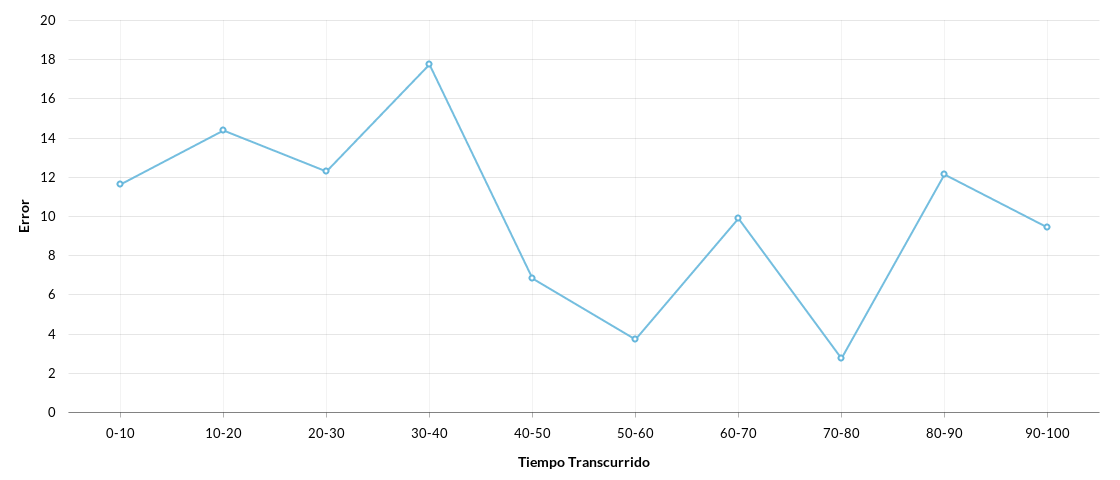
\includegraphics[width=1.0\linewidth]{./graphics/error_tiempo.png}
\caption{Distribuci\'on del Error Humano con respecto al Tiempo transcurrido}
\label{figure:gerror-tiempo}
\end{figure}


\section{Encuesta}
\label{sec:resultados-encuesta}

Luego de haber finalizado la tarea cuatro, cada sujeto complet\'o una encuesta de manera tal a
opinar sobre su experiencia interactuando con el sistema de reconocimiento de voz. 
En la tabla~\ref{sec:tabla-encuesta} se puede observar un resumen de la encuesta realizada.


\begin{table}[H] 
\centering
\footnotesize
\begin{tabular}{|r|r|r|r|r|}
\hline
    Sujeto & Palabras & Comandos & Entrenamiento & Interfaz por Voz \\
    \hline
    1 & 6 & 7 & 6 & 7 \\
    2 & 6 & 7 & 7 & 7 \\
    3 & 7 & 7 & 7 & 7 \\
    4 & 6 & 6 & 4 & 5 \\
    5 & 7 & 7 & 7 & 4 \\
    6 & 6 & 6 & 5 & 5 \\
    7 & 7 & 7 & 7 & 5 \\
    8 & 6 & 7 & 6 & 7  \\
    9 & 6 & 7 & 7 & 5  \\
    10 & 5 & 6 & 6 & 6  \\
    11 & 6 & 6 & 6 & 7  \\
    12 & 6 & 6 & 7 & 5  \\
\hline
\end{tabular}
\caption{Resumen de la encuesta realizada.}
\label{sec:tabla-encuesta}
\end{table}

La figura ~\ref{figure:kiviat-encuesta1} presenta los valores promediados para cada columna
de la tabla anterior mediante un gr\'afico radial.

\begin{figure}[ht]
\centering
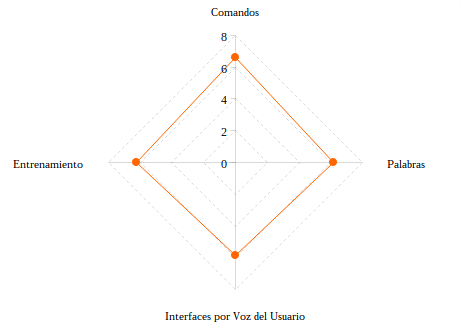
\includegraphics[width=0.6\linewidth]{./graphics/kiviat0.png}
\caption{Gr\'afico radial resumen de la encuesta realizada.}
\label{figure:kiviat-encuesta1}
\end{figure}

A continuaci\'on se presentan los resultados reescalados por usuario, en una escala del 0 al 1.


\begin{table}[H] 
\centering
\footnotesize
\begin{tabular}{|r|r|r|r|r|}
\hline
    Sujeto &  Palabras & Comandos & Entrenamiento & Interfaz por Voz \\
    \hline
1 &  0 & 1 & 0 & 1\\
2 &  0 & 1 & 1 & 1\\
3 &  - & - & - & -\\
4 &  1 & 1 & 0 & 0,5\\
5 &  1 & 1 & 1 & 0\\
6 &  1 & 1 & 0 & 0\\
7 &  1 & 1 & 1 & 0\\
8 &  0 & 1 & 0 & 1\\
9 &  0,5 & 1 & 1 & 0\\
10 & 0 & 1 & 1 & 1\\
11 & 0 & 0 & 0 & 1\\
12 & 0,5 & 0,5 & 1 & 0\\
\hline
\end{tabular}
\caption{Encuesta Reescalada.}
\label{sec:tabla-encuesta-normalizada}
\end{table}


La figura ~\ref{figure:kiviat-encuesta2} presenta los valores promediados para cada columna
de la tabla anterior mediante un gr\'afico radial. La misma permite observar el efecto del
cambio de escala, el cual facilita la identificaci\'on de fortalezas y debilidades. 

\begin{figure}[ht]
\centering
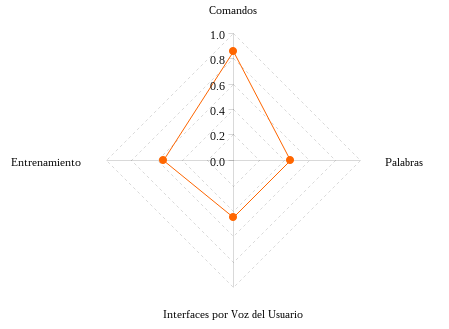
\includegraphics[width=0.6\linewidth]{./graphics/kiviat.png}
\caption{Gr\'afico radial resumen de la encuesta reescalada.}
\label{figure:kiviat-encuesta2}
\end{figure}


\appendix   % inician los apendices de tu tesis
	
% los cap'itulos que incluyas a partir de aqu'i aparecen 
% como ap'endices

% estos comandos generan la bilbiograf'ia
\printbibliography

\end{document}